%%===============================================================
%%===============================================================
%% Author: M Secanell
%%===============================================================
%%===============================================================
%%===============================================================
\documentclass[]{book}
%
% Created by Marc Secanell on May 18, 2010.
%
%-- For margins
\usepackage{fullpage}
\usepackage{simplemargins}
\setallmargins{1in}
%---
\usepackage{soul}
\usepackage{graphicx}
\usepackage{graphics}
\usepackage{placeins} %For Float Barriers
\usepackage{ulem} % Strike out \sout{}
\usepackage{listings}
\usepackage{multicol}
\usepackage{amsmath, amssymb, amsthm,epsf,subfig}
\usepackage[colorlinks=true]{hyperref}
\usepackage{alltt}

\lstset{ %
language=C++,                % choose the language of the code
basicstyle=\ttfamily\scriptsize,
keywordstyle=\color{blue}\ttfamily,
stringstyle=\color{red}\ttfamily,
commentstyle=\color{green}\ttfamily,       % the size of the fonts that are used for the code
numbers=left,                   % where to put the line-numbers
numberstyle=\footnotesize,      % the size of the fonts that are used for the line-numbers
stepnumber=1,                   % the step between two line-numbers. If it is 1 each line will be numbered
numbersep=5pt,                  % how far the line-numbers are from the code
backgroundcolor=\color{white},  % choose the background color. You must add \usepackage{color}
showspaces=false,               % show spaces adding particular underscores
showstringspaces=false,         % underline spaces within strings
showtabs=false,                 % show tabs within strings adding particular underscores
frame=single,           % adds a frame around the code
tabsize=2,          % sets default tabsize to 2 spaces
captionpos=b,           % sets the caption-position to bottom
breaklines=true,        % sets automatic line breaking
breakatwhitespace=false,    % sets if automatic breaks should only happen at whitespace
escapeinside={\%*}{*)}          % if you want to add a comment within your code
}


\newenvironment{changemargin}[2]{%
  \begin{list}{}{%
    \setlength{\topsep}{0pt}%
    \setlength{\leftmargin}{#1}%
    \setlength{\rightmargin}{#2}%
    \setlength{\listparindent}{\parindent}%
    \setlength{\itemindent}{\parindent}%
    \setlength{\parsep}{\parskip}%
  }%
  \item[]}{\end{list}} 

%opening
\title{{\Huge DRAFT: Open-source Fuel Cell Simulation Toolbox (OpenFCST)} \\
       { - \\}
       {\huge User's and Developer's Reference Guide}}      
\author{M.~Secanell, A.~Putz, V.~Zingan, M.~Bhaiya, M.~Moore,\\
        P.~Dobson, P.~Wardlaw, C.~Balen, A.~Kosakian,
        M.~Sabharwal and K.~Domican\\
		\\
        Energy Systems Design Laboratory\\
        University of Alberta, Canada}
\date{Created on: June 11, 2012 \\
      Last updated: \today}

\begin{document}

\maketitle

\tableofcontents

%%===============================================================
%%===============================================================
%%===============================================================
%%===============================================================
\chapter{Introduction}
%%===============================================================
%%===============================================================
% Authors: M. Secanell
%%===============================================================
\section{About OpenFCST}

The open-source Fuel Cell Simulation Toolbox (OpenFCST) is an open-source mathematical modelling package for polymer electrolyte fuel cells. OpenFCST has been developed as a modular toolbox from which you can develop your own applications. It contains a database of physical phenomena equations, fuel cell layers and materials, and mathematical models for reaction kinetics. In addition, it already contains several applications that allow you to simulate different fuel cell components. For example, you can simulate a cathode electrode (using either a macrohomogeneous or an ionomer-filled agglomerate model), an anode electrode or a complete membrane electrode assembly. The applications already provided in OpenFCST have been validated with respect to experimental data in the literature \cite{Dobson12} as well as numerical results from other models implemented in a commercial package~\cite{Secanell07}. A thorough description of the model and validation is presented in \cite{Secanell07}.

OpenFCST is being developed at the \htmladdnormallink{Energy Systems Design Laboratory}{http://secanell-srv01.mece.ualberta.ca/} at the University of Alberta in collaboration with the \htmladdnormallink{Automotive Fuel Cell Cooperation Corp.}{http://www.afcc-auto.com} that, together with the \htmladdnormallink{Natural Science and Engineering Research Council of Canada}{www.nserc-crsng.gc.ca}, has provided the majority of the funding required to develop this code. The goal of OpenFCST is that research groups in academia and in industry use the current toolbox to better understand fuel cells and to develop new physics and material databases that can then be integrated in the current library.

OpenFCST is an integrated open-source tool for fuel cell analysis and design. It seamlessly integrates several open-source pre-processing, finite element, and post-processing tools in order to analyze fuel cell systems. OpenFCST contains a built-in mesh generator. If your problem requires you to simulate more complex geometries, it can also import quadrilateral meshes generated with the open-source pre-processor \htmladdnormallink{Salome}{http://www.salome-platform.org/} and exported in UNV format. The physics and material database in OpenFCST allows you to setup the governing equations for the most important physical processes that take place in a fuel cell. OpenFCST already implements the weak form for many governing equations. They are solved using the finite element open-source library \htmladdnormallink{deal.II}{http://www.dealii.org/}. OpenFCST builds on top of the \htmladdnormallink{deal.II}{http://www.dealii.org/} finite element libraries and many of its software requirements and coding philosophy is inherited from deal.II. In order to analyze your results, OpenFCST can output your results to .vtu files that can easily be read with the open-source post-processor \htmladdnormallink{Paraview}{http://www.paraview.org/}. OpenFCST is also integrated with the design and optimization package \htmladdnormallink{Dakota}{http://dakota.sandia.gov/software.html}. Therefore, it can be used for design and optimization as well as parameter estimation~\cite{Secanell07,Secanell07b,Secanell08,Dobson12}.

OpenFCST is under development. If you like the library and would like to contribute towards the development, you can help the developers in the following ways:
\begin{itemize}
 \item If you are an industrial researcher that is considering using OpenFCST for research and development in the company, please contact the developers in order to develop a research program with them. 
 \item If you are either an industrial or academic researcher using the library, please make sure to cite the OpenFCST libraries in your publications. Please cite any relevant publication by the OpenFCST developers as well as the current reference \cite{Secanell13} and introduction paper \cite{Secanell14}.
 \item If you are either an industrial or academic researcher using the library and you have developed a new physics model or material database entry, please consider submitting it to the developers so that it can be integrated with the newest version of OpenFCST.
 \item If you are an industrial researcher considering using OpenFCST for research and development in the company, please consider hiring the graduate students that develop OpenFCST, i.e. the graduate   students from the \htmladdnormallink{Energy Systems Design Laboratory}{http://secanell-srv01.mece.ualberta.ca/?q=people} at the University of Alberta.
\end{itemize}

Currently, the developers are working on:
\begin{itemize}
 \item improving the code readability – new classes are being developed for making the code easier to understand and more modular;
 \item developing a convective gas and liquid transport model for the electrodes;
 \item developing a Navier-Stokes solver for gas transport in the fuel cell channels.
\end{itemize}

\section{About the Developers}

OpenFCST was originally conceived by M. Secanell in 2006 while doing his Ph.D. at the University of Victoria~\cite{Secanell07}. In 2004, M. Secanell developed a small set of routines that were used to setup the governing equations for a fuel cell cathode in two dimensions. The governing equations were first linearized and then the weak form of the equations was implemented and solved using the \htmladdnormallink{deal.II}{http://www.dealii.org/} finite element libraries \cite{Secanell07b}. In 2006, after attending a deal.II workshop in Heidelberg, Germany, and discussing the idea of creating an open-source code for fuel cells based on deal.II with Dr. Guido Kanschat and Dr. Wolfgang Bangerth, M. Secanell decided to integrate the routines he had developed into AppFrame, an application framework developed by Dr. Guido Kanschat, thereby initiating the development of a toolbox that could be used to create modules or applications for fuel cell analysis. From 2006 to 2008, OpenFCST development continued with the implementation of a complete membrane electrode assembly model; however, with M. Secanell as a sole developer, the code was too rough and disorganized to result in an open-source fuel cell package that the research community could use. In 2009, once M. Secanell joined the University of Alberta, the idea of developing OpenFCST was solidified. Thanks to the funding provided by the \htmladdnormallink{Automotive Fuel Cell Cooperation Corp.}{http://www.afcc-auto.com/}, \htmladdnormallink{MITACS}{http://www.mitacs.ca/} and the \htmladdnormallink{Natural Science and Engineering Research Council of Canada}{http://www.nserc-crsng.gc.ca}, a group of core developers was established at the \htmladdnormallink{Energy Systems Design Laboratory}{http://secanell-srv01.mece.ualberta.ca/} at the University of Alberta. The current research team re-developed the majority of the classes in order to increase the modularity, usability and reliability of the code. Currently, OpenFCST is used by 6-8 researchers at two different laboratories, it is 
tested nightly for errors and it contains a bug tracking site to report any issues with its performance.

The current group of OpenFCST developers is formed by:
\begin{itemize}
 \item M. Secanell, Associate Professor, Energy Systems Design Laboratory, University of Alberta, Canada 
   \subitem Responsible for overall framework (base class concepts), optimization interface, electronic, protonic, membrane water transport, Fick's gas transport and kinetics
 \item A. Putz, Senior Research Scientist, Automotive Fuel Cell Cooperation Corp. 
   \subitem Responsible for plug-points and AFCC contributions
 \item V. Zingan, Post-doctoral Fellow, Energy Systems Design Laboratory, University of Alberta, Canada 
   \subitem Responsible for overall framework (base class concepts), Navier-Stokes, Darcy and multi-component fluid flow physical models and applications
 \item M. Bhaiya, M.Sc. student, Energy Systems Design Laboratory, University of Alberta, Canada 
   \subitem Responsible for overall framework (base class concepts) and thermal physical models and applications
 \item P. Wardlaw, M.Sc. student, Energy Systems Design Laboratory, University of Alberta, Canada 
   \subitem Responsible for installation script and multi-scale framework (1D agglomerate models)
 \item K. Domican, M.Sc. student, Energy Systems Design Laboratory, University of Alberta, Canada 
   \subitem Responsible for optimization interface and documentation
 \item C. Balen, M.Sc. student, Energy Systems Design Laboratory, University of Alberta, Canada 
   \subitem Responsible for the development of the installation script and CMake scripts
 \item J. Zhou, Ph.D. student, Energy Systems Design Laboratory, University of Alberta, Canada 
   \subitem Responsible for the development of a two-phase flow application (for release 1.0)
 \item M. Sabharwal, M.Sc. student, Energy Systems Design Laboratory, University of Alberta, Canada 
   \subitem Responsible for the development of micro-scale simulation applications, e.g. appDiffusion
 \item A. Kosakian, Ph.D. student, Energy Systems Design Laboratory, University of Alberta, Canada 
   \subitem Responsible for the development of domain decomposition strategies (for release 1.0)
\end{itemize}
Other scientists that have also contributed substantial portions of code to OpenFCST are:
\begin{itemize}
 \item M. Moore, M.Sc. graduate from the Energy Systems Design Laboratory, University of Alberta, Canada 
   \subitem Responsible for installation script, double-trap kinetics model for ORR reaction and multi-scale framework (1D agglomerate models)
 \item G. Kanschat, Universität Heidelberg
  \subitem Developer of AppFrame (now part of OpenFCST application\_core routines)
 \item P. Dobson, M.Sc. graduate from the Energy Systems Design Laboratory
    \subitem Developed parts of overall framework (base class concepts), optimization interface and multi-scale framework (1D agglomerate models)
 \item A. Malekpourkoupaei, former M.Sc. graduate student at the Energy Systems Design Laboratory
    \subitem Developed classes PureGas and classes to compute binary diffusivity (together with M. Secanell)
\end{itemize}


\section{License}

The Fuel Cell Simulation Toolbox (OpenFCST) is distributed under the MIT License.

Copyright (C) 2013-15 Energy Systems Design Laboratory, University of Alberta

The MIT License (MIT)

Permission is hereby granted, free of charge, to any person obtaining a copy of this software 
and associated documentation files (the "Software"), to deal in the Software without restriction, 
including without limitation the rights to use, copy, modify, merge, publish, distribute, 
sublicense, and/or sell copies of the Software, and to permit persons to whom the Software 
is furnished to do so, subject to the following conditions:

The above copyright notice and this permission notice shall be included in all 
copies or substantial portions of the Software.

THE SOFTWARE IS PROVIDED "AS IS", WITHOUT WARRANTY OF ANY KIND, EXPRESS OR IMPLIED, 
INCLUDING BUT NOT LIMITED TO THE WARRANTIES OF MERCHANTABILITY, FITNESS FOR A PARTICULAR 
PURPOSE AND NONINFRINGEMENT. IN NO EVENT SHALL THE AUTHORS OR COPYRIGHT HOLDERS BE LIABLE 
FOR ANY CLAIM, DAMAGES OR OTHER LIABILITY, WHETHER IN AN ACTION OF CONTRACT, TORT OR OTHERWISE, 
ARISING FROM, OUT OF OR IN CONNECTION WITH THE SOFTWARE OR THE USE OR OTHER DEALINGS IN THE SOFTWARE.

\section{Release notes} \label{main_changes}

New in release 0.2:
\begin{itemize}
 \item New graphical user interface (GUI)
 \item Non-isothermal membrane electrode assembly model (see M. Bhaiya, A. Putz and M. Secanell, "Analysis of non-isothermal effects on polymer electrolyte fuel cell electrode assemblies", Electrochimica Acta, 147C:294-309, 2014. DOI: 10.1016/j.electacta.2014.09.051)
  \item Double-trap kinetic model (see M. Moore, A. Putz and M. Secanell, "Investigation of the ORR Using the Double-Trap Intrinsic Kinetic Model", Journal of the Electrochemical Society 160(6): F670-F681. doi: 10.1149/2.123306jes)
  \item Multi-scale framework for analysis of complex agglomerate structures (see M. Moore, P. Wardlaw, P. Dobson, J.J. Boisvert, A. Putz, R.J. Spiteri, M. Secanell, "Understanding the Effect of Kinetic and Mass Transport Processes in Cathode Agglomerates", Journal of The Electrochemical Society, 161(8):E3125-E3137 DOI: 10.1149/2.010408jes)
  \item Improved compilation script and transition to CMake: OpenFCST will automatically look for all dependent libraries and download any missing libraries if necessary (installation tested nightly in OpenSUSE 13.1, 13.2, and Ubuntu 14.04)
  \item Improved documentation: Improved user guide and folder with input files for several of the articles above
  \item Improved post-processing capabilities: New classes developed to be able to output oxide coverage, agglomerate effectiveness, relative humidity, overpotentials and more
  \item Improved post-processing capabilities: New classes to compute functionals such as overall current density and all types of heat losses
\end{itemize}

%%===============================================================
%%===============================================================
%%===============================================================

%%===============================================================
\part{User's Guide}
%%===============================================================
%%===============================================================
\chapter{Installation}
%%===============================================================
%%===============================================================
% Authors: M. Secanell and Chad Balen.
%%===============================================================

%%===============================================================
\section{Downloading OpenFCST}
%%===============================================================

\subsection{Users}

\subsubsection{Download a .tar file}
OpenFCST can be found at the  \htmladdnormallink{OpenFCST}{http://www.openfcst.org/} website. In the download section you will be able to find and download a .tar file of the latest release. 

\subsubsection{Download from GitHub}
The latest release of OpenFCST can also be downloaded from \htmladdnormallink{OpenFCST}{https://github.com/OpenFcst/OpenFcst0.2} on GitHub.


%%===============================================================
\section{Installing OpenFCST} \label{installing_fcst}
%%===============================================================

\subsection{System requirements}

OpenFCST is developed on Linux and compiled using the GCC compiler. OpenFCST developers perform nightly compilation tests on the following operating systems:
\begin{itemize}
 \item OpenSUSE 13.1 (evergreen) and 13.2;
 \item Ubuntu 14.04.1 (long time support).
\end{itemize}
These are the operating systems that the OpenFCST developers recommend. 

If you would like to try to run the code under Windows environment, our recommendation is to install a VirtualBox with OpenSUSE and then, install and run OpenFCST on the virtual machine.

The following software needs to also be installed in your computer in order for OpenFCST to compile:
\begin{itemize}
 \item GNU make and C++11 support, gcc version 4.7 or later (4.8.1 Recommended)
 \item GCC
 \item BLAS and LAPACK libraries 
 \item OpenMPI compiler
 \item gfortran compiler
 \item Bison
 \item qt4-designer and libqt4
 \item For generating the documentation: DOxygen and Sphinx
 \item Boost; the specific packages are iostreams, serialization, system, thread, 
       filesystem, regex, signals, \& program\_options)
 \item FLEX (For Dakota)
 \item Python Packages: SciPy, NumPy, ipython, Sphinx, evtk, vtk, mayavi, matplotlib(with backends)
 \item libconfig-devel and libconfig++-devel
\end{itemize}

In addition, the following packages might be useful if you are planning on developing new classes for OpenFCST:
\begin{itemize}
  \item For debugging programs, we have found that the GNU debugger GDB is an invaluable tool. GDB is a text-based tool not always easy to use; kdbg is one of many graphical user interfaces for it. \item Most integrated development environments like KDevelop or Eclipse have built in debuggers as well.
\end{itemize}

If you check the OpenFCST folder, you will find install scripts for OpenSUSE and Ubuntu
to help install all necessary packages.

\subsection{OpenSUSE 13.1 and 13.2}
Before running OpenFCST on a new machine if Sphinx is installed then in terminal go into src/examples/ and 
execute the dependencies.sh file. This will install all necessary python dependencies. 

\subsection{Ubuntu 14.04}
To install necessary packages on Ubuntu 14.04 please execute the openFCST\_install\_Ubuntu1404.sh script through terminal.

\subsection{Installation steps}
Fuel Cell Simulation Toolbox is a fuel cell simulation package developed using several open-source libraries 
such as the deal.II libraries, DAKOTA and COLDAE. In order to run 
without any difficulties, OpenFCST needs to compile and link to all these applications which are provided with 
the code in the folder src/contrib. Please note that each package is distributed under a different license. 

OpenFCST contains a script to compile all packages simultaneously. To compile OpenFCST and all other libraries use the following:
\begin{lstlisting}
$./openFCST_install --with-dakota --cores=4
\end{lstlisting}

If some packages such as p4est, METIS, and PETSc are not in the src/contrib folder, then OpenFCST will download them from the Internet for you.  Since Dakota is not automatically installed you must specify the flag shown above for OpenFCST to install Dakota. Then CMake will install it and make the necessary changes to it, so Dakota works with OpenFCST. Since MPI is mandatory and CMake finds OpenMPI for you we do not need to specify any flag to tell CMake where to find it.
Finally, we select to compile on four cores to speed up the compilation process. 

The install script assumes the default path for the OpenMPI compiler and that all the libraries are in \texttt{src/contrib}. If you already have a version of deal.II and you would like to use that version, use the flags \texttt{--deal-dir}. Please check the src/README for any necessary changes that must be made to deal.ii for it to work with OpenFCST. For more information on the script options, type
\begin{lstlisting}
$./openFCST_install --help
\end{lstlisting}

%%===============================================================
%%===============================================================
%%===============================================================
%%===============================================================
\chapter{OpenFCST structure}
%%===============================================================
%%===============================================================
% Authors: M. Secanell and Chad Balen.
%%===============================================================

Prior to installation, OpenFCST contains the following main folders:
\begin{itemize}
 \item \texttt{src} contains all source files for OpenFCST, documentation files, licenses and this guide;
 \item \texttt{pre\_processing} contains a collection of additional programs to improve the usability of OpenFCST such as a collection of Python scripts for Salome;
 \item \texttt{post\_processing} contains a collection of additional Python scripts to further post-process the results obtained using OpenFCST with ParaView; 
 \item \texttt{python} contains a collection of Python scripts for plotting polarization curves and further post-processing of the solution.
\end{itemize}

After installation of OpenFCST, two additional folders will appear:
\begin{itemize}
 \item \texttt{Install} contains the binaries of OpenFCST. \textbf{OpenFCST users should only work in this folder};
 \item \texttt{Build} contains auxiliary files necessary for the compilation of OpenFCST. This folder is therefore of no interest to users of OpenFCST.
\end{itemize}

The \texttt{Install} folder is the only folder users should be concerned with. Users should think of \texttt{Install} as installation folder, i.e. the folder where all files necessary to execute OpenFCST are installed. Other folders contain either source code for OpenFCST, i.e. \texttt{src} and \texttt{python}, or auxiliary routines that are not critical to OpenFCST. In the remaining of the User Manual, we will assume that users have installed the program and they are working from the \texttt{Install} directory.

%%===============================================================
\section{Install directory tree}
%%===============================================================
The Install directory of OpenFCST contains two scripts and nine subfolders. The subfolders are namely:
\begin{itemize}
 \item \texttt{bin} contains binary executable files for OpenFCST. The main three executables are: a)~\texttt{fuel\_cell-2d.bin}, b)~\texttt{fuel\_cell-3d.bin}, and c)~\texttt{fcst\_gui}. The first file is used to run OpenFCST through the terminal for solving 2D problems, the second for running 3D problems, and the last file is the file to execute the graphical user interface. 
 \item \texttt{examples} contains a set of example problems to learn how to use OpenFCST. In particular, there are examples to simulate a cathode, a membrane electrode assembly (MEA) with macro-homogeneous and agglomerate models, and a non-isothermal MEA. The files in the example folder should not be modified. Instead, copy the appropriate files to \texttt{my\_data} and modify as necessary.
 \item \texttt{doc} contains all documentation except for the examples. This includes:
 \begin{itemize}
  \item a main HTML page, i.e., \texttt{index.html}, that can be used to access all documentation in OpenFCST;
  \item the User’s Manual in PDF and \TeX format (in \texttt{RefGuide} folder);
  \item the class documentation in HTML and \TeX, i.e. the documentation for each routine developed in OpenFCST (in \texttt{html} and \texttt{latex} folders).
 \end{itemize}
 \item \texttt{contrib} contains the contributing libraries to OpenFCST. These are libraries that have been developed by other people and are used within OpenFCST. They include deal.II and DAKOTA. Note that some of these libraries have been slightly modified by OpenFCST developers (see README file in each subfolder).
 \item \texttt{databases} contains databases used in the case of numerical agglomerates to speed-up OpenFCST simulations. If you are not using a numerical agglomerate model, you do not need to worry about this folder.
 \item \texttt{fcst} contains the .h files needed in order to link other libraries to OpenFCST. This folder is not necessary for Users.
 \item \texttt{test} contains the configuration files used to run the tests to make sure the OpenFCST has been installed correctly. These same files are used with CDash to make sure OpenFCST continues to provide the same results between releases.
 \item \texttt{python} contains a collection of Python scripts to help with post-processing. This section is in its infancy.
 \item \texttt{my\_data} does not contain any information. It is created to allow users to store their simulation data.
\end{itemize}

The two scripts are \texttt{fcst\_env.sh} and \texttt{run\_tests}. The first file should be executed when you start the program. It contains environment variable definitions for OpenFCST. This file can be copied directly to your \texttt{.bash\_profile} so that the variables are always defined. The definition of environment variables is needed for successful passing of all tests. To source the file, type the following:
\begin{lstlisting}
. fcst_env.sh
\end{lstlisting}
The second file, \texttt{run\_tests}, is a script used to execute all examples in the example folder. The results are compared to pre-computed results in order to make sure OpenFCST is running correctly on your system.

%%===============================================================
%%===============================================================
%%===============================================================
%%===============================================================
\chapter{Pre-processor}
%%===============================================================
%%===============================================================
%%===============================================================
% Authors: V. Zingan and Chad Balen.
%%===============================================================

In order to generate a fuel cell domain using OpenFCST, two options are available:
\begin{itemize}
 \item use the classes under \texttt{FuelCell::Geometry} namespace;
 \item read in a mesh generated using an open-source mesh generator such as Salome;
\end{itemize}

%%===============================================================
\section{\texttt{FuelCellShop::Geometry} Namespace}
Namespace \texttt{FuelCellShop::Geometry} contains classes to generate a cathode and anode fuel cell electrode, a spherical agglomerate, and a membrane electrode assembly with five or seven layers (i.e. with and without micro porous layer). To use these classes, you simply need to create an object of the class. Then, use the declare\_parameters member function to define the variables required in the input file, initialize the object calling initialize and generate the grid using generate\_grid. For example,
\begin{lstlisting}
//Create object
FuelCellShop::Geometry::PemfcMPL<dim> grid; 
//Declare the necessary variables in the ParameterHandler deal.ii object
grid.declare_parameters(param);         
//Once the ParameterHandler object has been initialized by reading from file, 
//initialize the geometry varialbes 
grid.initialize(param);                 
//Generate the mesh and store it in the dealii::Triangularization variable tr  
grid.generate_grid(*this->tr);          
\end{lstlisting}

%%===============================================================
\section{Developing a mesh in Salome}
SALOME is an open-source cross-platform software that provides a generic platform for Pre-Processing. It is distributed under the terms of the GNU LGPL license. You can download both source code and executable files from the \htmladdnormallink{Salome site}{http://www.salome-platform.org/}.

%%=======
\subsection{Tutorial}
This short tutorial demonstrates how to create a simple mesh in Salome 7.3.0, define material and boundary indicators, and adapt all of this to the needs of the OpenFCST library.

The object we would like to mesh is represented by a two dimensional H-shaped domain as shown in Figure~\ref{fig:no3.2.1.1}.

\begin{figure}[tbp]
\begin{center}
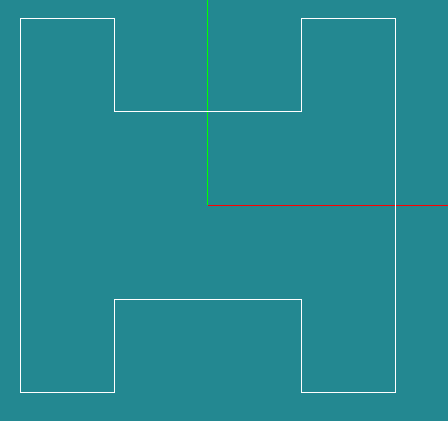
\includegraphics[width=0.43\textwidth]{figures/salome0.png}
\caption{H-shaped domain.}
\label{fig:no3.2.1.1}
\end{center}
\end{figure}

OpenFCST only accepts meshes composed of either quadrilaterals in 2D or hexahedrals in 3D. \textbf{OpenFCST assumes that all the geometrical dimensions are in centimeters}. The current version of Salome is only able to produce these type of meshes with geometries that have an outer boundary composed exactly of 4 pieces in 2D, e.g. see Figure~\ref{fig:no3.2.1.2}, and 6 pieces in 3D, e.g see Figure~\ref{fig:no3.2.1.3}. In order to increase the quadrilateral and hexahedral properties of Salome however, a commercial package called Hexotic is distributed by Distine (for more information, please visit the \htmladdnormallink{site}{http://www-roc.inria.fr/gamma/gamma/Membres/CIPD/Loic.Marechal/Research/Hexotic.html}).

\begin{figure}[tbp]
\begin{center}
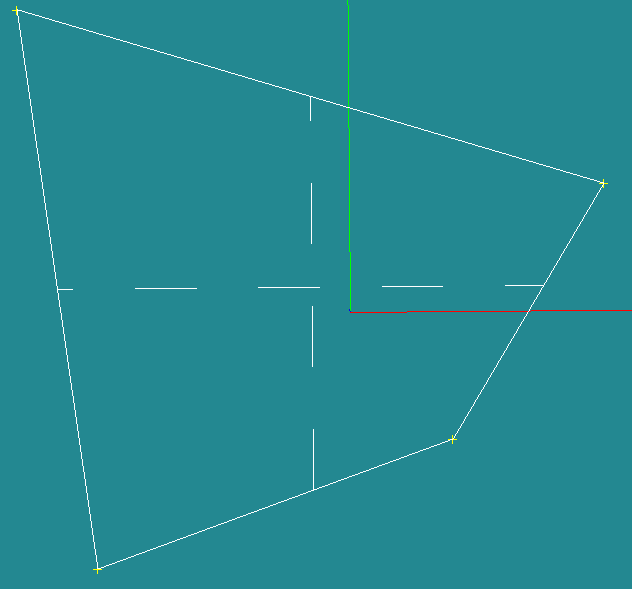
\includegraphics[width=0.43\textwidth]{figures/salome01.png}
\caption{Linear quadrilateral.}
\label{fig:no3.2.1.2}
\end{center}
\end{figure}

\begin{figure}[tbp]
\begin{center}
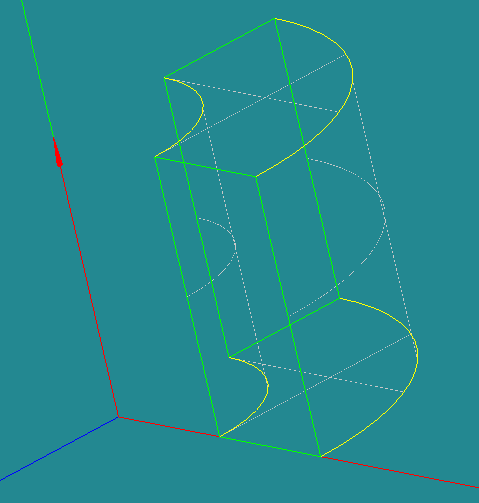
\includegraphics[width=0.43\textwidth]{figures/salome02.png}
\caption{Quarter of cylindrical shell.}
\label{fig:no3.2.1.3}
\end{center}
\end{figure}

The two dimensional H-shaped domain shown in Figure~\ref{fig:no3.2.1.1} has 12 pieces for the outer boundary and hence can not be meshed in Salome directly by means of quadrilaterals. We can mesh the domain however by splitting it into 3 parts, such that each of the parts has 4 outer boundary segments. Then, we mesh each of these parts and combine them into the H-shaped domain.

Let us do this step by step:

\subsubsection{Creating a geometric entity}

Run Salome, select \textbf{New document}, and then select \textbf{Geometry} on the upper toolbox (Figure \ref{fig:no3.2.1.4}). 

\begin{figure}[tbp]
\begin{center}
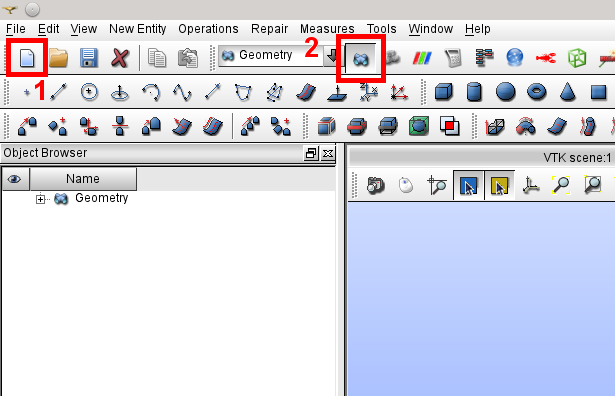
\includegraphics[scale=0.60]{figures/SalomeStep1.png}
\caption{Starting a New Project.}
\label{fig:no3.2.1.4}
\end{center}
\end{figure}
  
We are now in the Geometry module of Salome, and the first thing we need to do is to define 12 vertices along the object: 
\begin{itemize}
 \item 1(-1, -1)
 \item 2(-0.5, -1)
 \item 3(-0.5, 1)
 \item 4(-1, 1)
 \item 5(-0.5, -0.5)
 \item 6(0.5, -0.5)
 \item 7(0.5, 0.5)
 \item 8(-0.5, 0.5)
 \item 9(0.5, -1)
 \item 10(1, -1)
 \item 11(1, 1)
 \item 12(0.5, 1)
\end{itemize}
To create any of these points, we go to \textbf{New Entity} $\rightarrow$ \textbf{Basic} $\rightarrow$ \textbf{Point}, specify a \textbf{Name} and the respective fields \textbf{X:}, \textbf{Y:}, and \textbf{Z:}, then select \textbf{Apply}. For the last vertex use the \textbf{Apply and Close} button instead of Apply. Note that instead of \textbf{New Entity} $\rightarrow$ \textbf{Basic} $\rightarrow$ \textbf{Point} we can simply choose \textbf{Create a point} on the upper toolbox. After initializing all the points select the -OZ view button to change the view and zoom into our geometry (Figure \ref{fig:no3.2.1.5}).

\begin{figure}[tbp]
\begin{center}
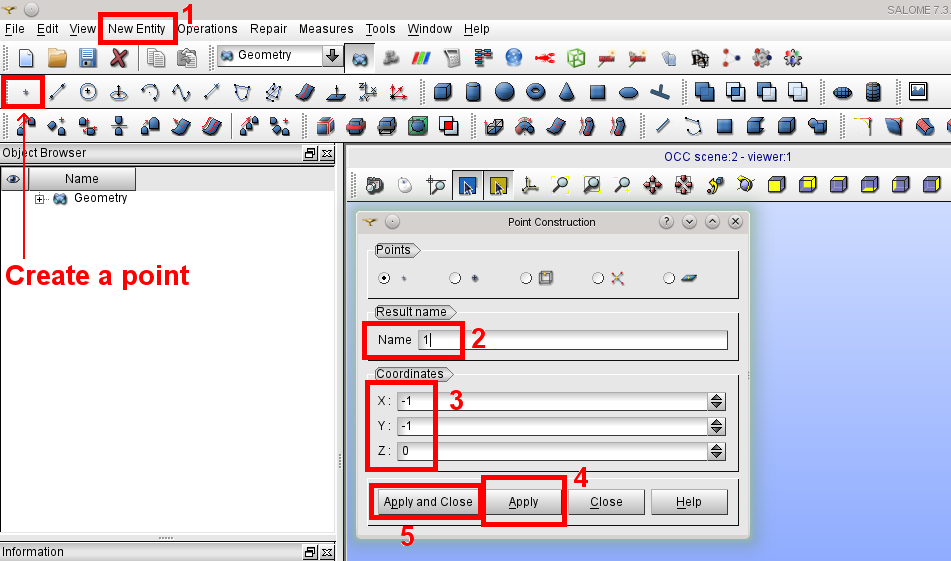
\includegraphics[scale=0.50]{figures/SalomeStep1b.png}
\caption{Creating a Point.}
\label{fig:no3.2.1.5}
\end{center}
\end{figure}

Next we create 3 quadrangle faces. Each of these faces consists of 4 points:
\begin{itemize}
 \item 1(1, 2, 3, 4)
 \item 2(5, 6, 7, 8)
 \item 3(9, 10, 11, 12).
\end{itemize}

To create a quadrangle face, we go to \textbf{New Entity} $\rightarrow$ \textbf{Blocks} $\rightarrow$ \textbf{Quadrangle Face}, fill out the fields \textbf{Vertex 1}, \textbf{Vertex 2}, \textbf{Vertex 3}, and \textbf{Vertex 4} with the points from above, and select \textbf{Apply and Close} button (Figure \ref{fig:no3.2.1.7}). To prevent possible problems always specify vertices in a counter-clockwise direction.

\begin{figure}[tbp]
\begin{center}
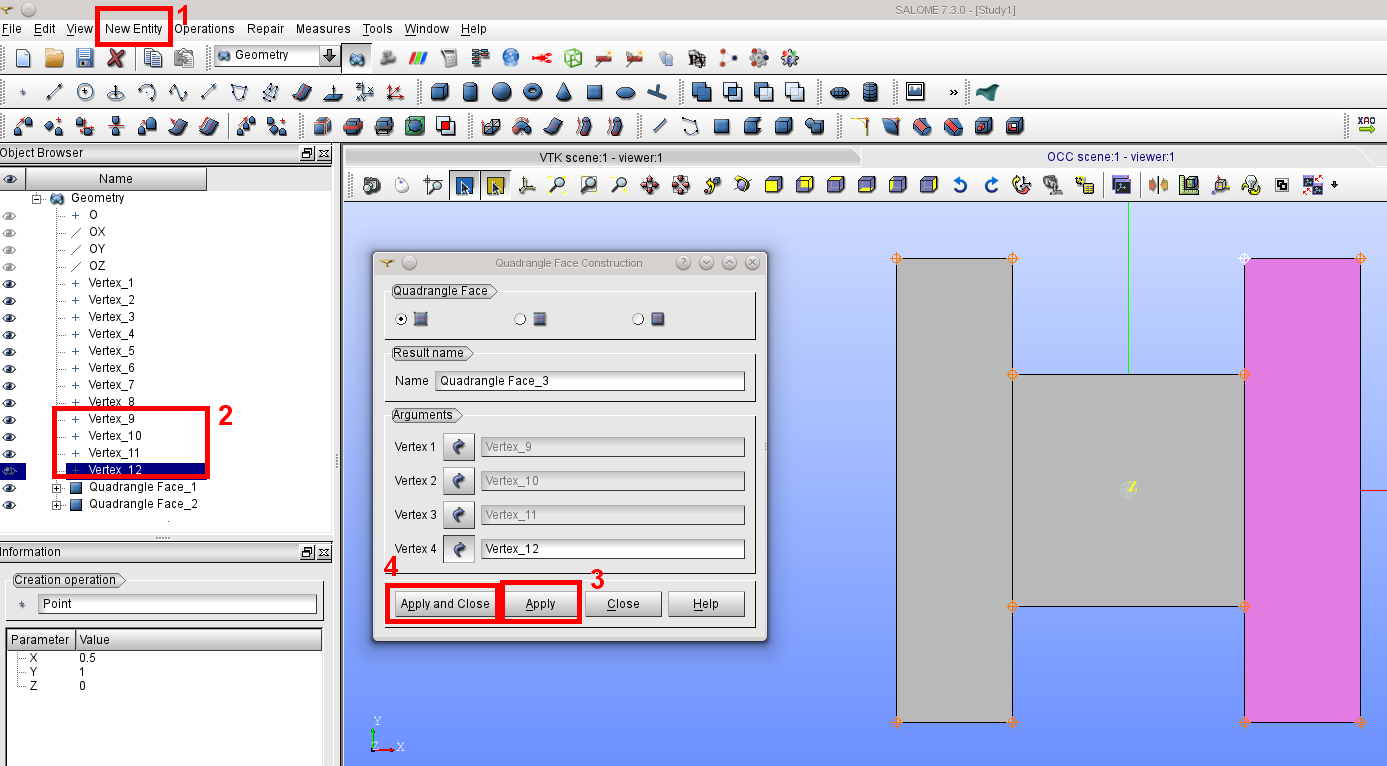
\includegraphics[scale=0.4]{figures/SalomeStep2.png}
\caption{Creating a Quadrangle Face.}
\label{fig:no3.2.1.7}
\end{center}
\end{figure}

\subsubsection{Generating a mesh for each domain}

At this point we have created our geometry. We now would like to generate the mesh. For this, we switch our attention to the Mesh module. To enter the Mesh module, select the \textbf{Mesh} button on the upper toolbox. To create an appropriate mesh on each of the quadrangle faces, we go to \textbf{Mesh} $\rightarrow$ \textbf{Create Mesh}, where we pass the respective quadrangle face to the \textbf{Geometry} field. Once this is done, we select \textbf{Quadrangle (Mapping)} from the drop-down menu of the \textbf{Algorithm} field (Figure \ref{fig:no3.2.1.9}).

\begin{figure}[tbp]
\begin{center}
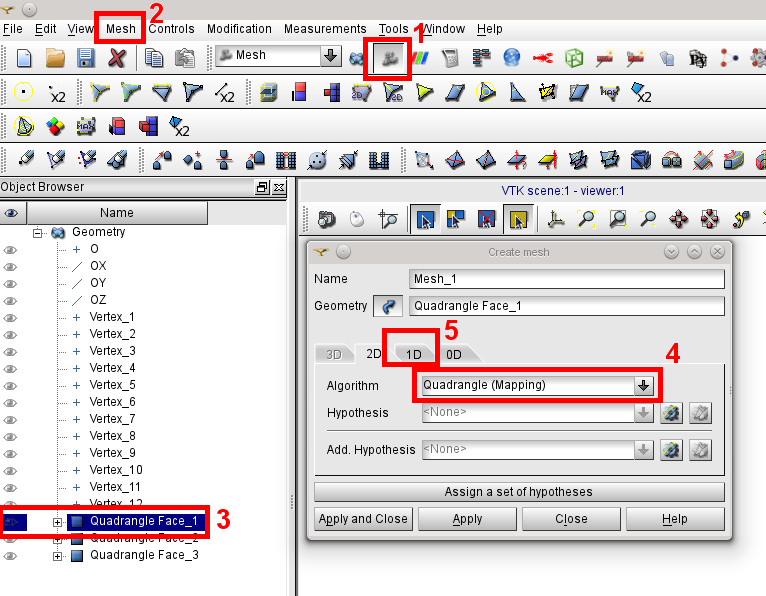
\includegraphics[scale=0.50]{figures/SalomeStep3.png}
\caption{Creating a Mesh.}
\label{fig:no3.2.1.9}
\end{center}
\end{figure}

After that we select the \textbf{1D} tab and check that \textbf{Algorithm} is set up to \textbf{Wire discretization}. The number of 1D hypotheses is available here. We choose the one which is called \textbf{Local Length}. This method uses a uniform spacing between nodal mesh points to generate the mesh on the selected edge. Set the \textbf{Length} parameter to 0.5 as shown in Figure \ref{fig:no3.2.1.10}.

\begin{figure}[tbp]
\begin{center}
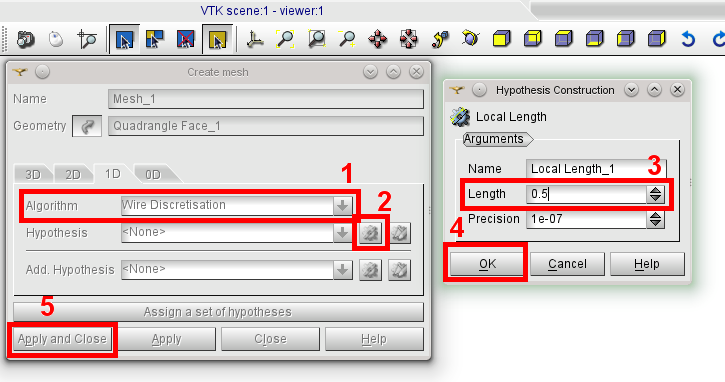
\includegraphics[scale=0.50]{figures/SalomeStep3b.png}
\caption{Setting Mesh Parameters.}
\label{fig:no3.2.1.10}
\end{center}
\end{figure}

After clicking \textbf{OK}, the name of the \textbf{Hypothesis} field should change to \textbf{Local Length\_1}. Then \textbf{Apply and Close}. Right click on the \textbf{Mesh\_1} and \textbf{Compute}. After applying this strategy to all the quadrangle faces and selecting the -OZ view button again, we have something like Figure \ref{fig:no3.2.1.11}.

\begin{figure}[tbp]
\begin{center}
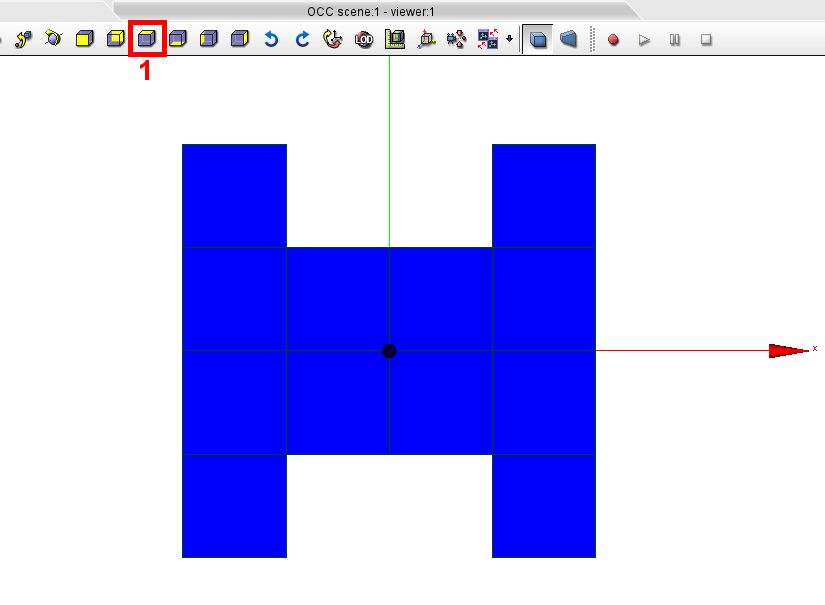
\includegraphics[scale=0.60]{figures/SalomeStep3c.png}
\caption{Overview of the Mesh.}
\label{fig:no3.2.1.11}
\end{center}
\end{figure}

At this point we have generated one mesh for each geometrical entity. These meshes still need to be combined into an overall mesh. Furthermore, we might want to identify each geometrical entity and boundary with an indicator so that we can apply different properties in each domain.

\subsubsection{Assigning material and boundary IDs to different parts of the mesh and creating an overall mesh}

Let us now assign Material IDs to all the cells we have created. \textbf{Material IDs in OpenFCST need to be unsigned integers}, so please do not use names as material IDs. Let us assign all the cells of Mesh\_1 a Material ID = 1, those belonging to Mesh\_2 a Material ID = 2, and cells from Mesh\_3 a Material ID = 3. To assign the material IDs, right click on \textbf{Mesh\_1}, then select \textbf{Create Group}. On this dialog box specify an \textbf{Element Type} of \textbf{Face}, \textbf{Name} of 1,\textbf{Select All}, and finally \textbf{Apply and Close} (Figure \ref{fig:no3.2.1.12}). Repeat this process for the other Material IDs.

\textit{Tip:} If you wish to use the \textbf{Manual Selection} option to add the cells to the \textbf{Id Elements} field, push and hold the Shift key on your keyboard and select the cells by left clicking. After all the desired cells have been highlighted, select \textbf{Add} in the Create Group dialog window.

\begin{figure}[tbp]
\begin{center}
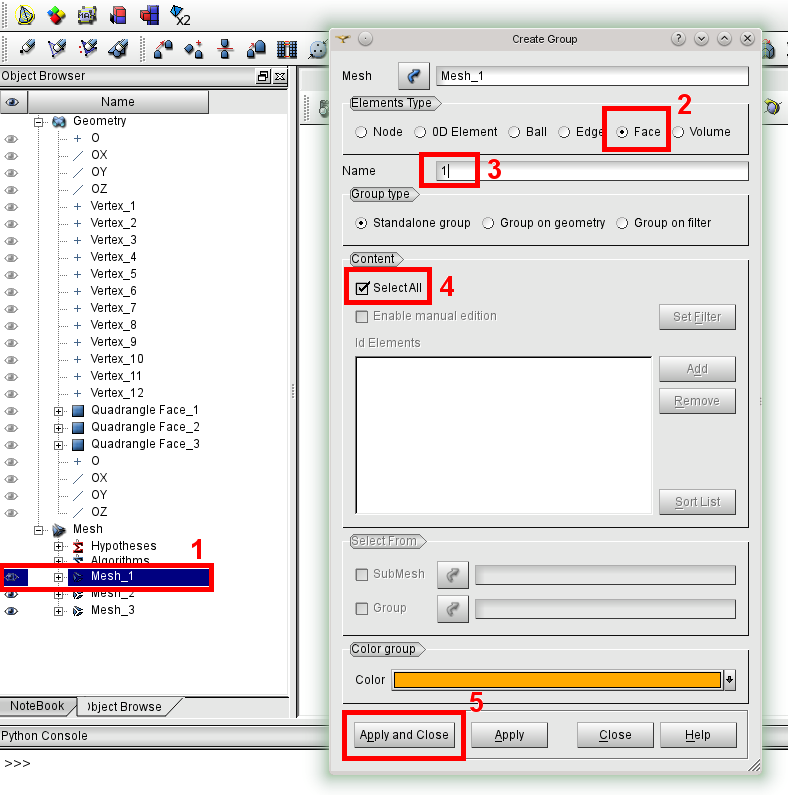
\includegraphics[scale=0.50]{figures/SalomeStep4.png}
\caption{How to Set the Material ID.}
\label{fig:no3.2.1.12}
\end{center}
\end{figure}

Now create a Compound Mesh by simply merging all the previously created meshes. This is done by selecting all the meshes, then from the toolbox \textbf{Mesh} $\rightarrow$ \textbf{Build Compound}. Specify a \textbf{Name}, select \textbf{Create common groups for initial meshes} and \textbf{Merge coincident nodes and elements}, and finally select \textbf{Apply and Close} (Figure \ref{fig:no3.2.1.13}).
        
\begin{figure}[tbp]
\begin{center}
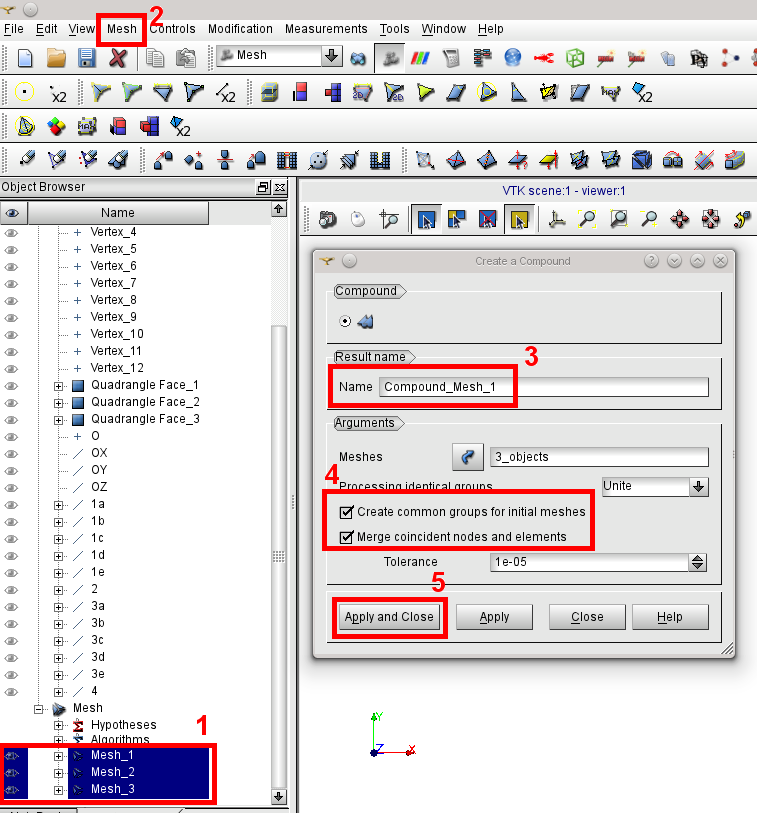
\includegraphics[scale=0.50]{figures/SalomeStep5.png}
\caption{Building a Compound Mesh.}
\label{fig:no3.2.1.13}
\end{center}
\end{figure}

In the \textbf{Object Browser} expand the \textbf{Compound\_Mesh\_1} and delete all groups except for the Material IDs in the \textbf{Groups of Faces} (Figure \ref{fig:no3.2.1.15}).
        
\begin{figure}[tbp]
\begin{center}
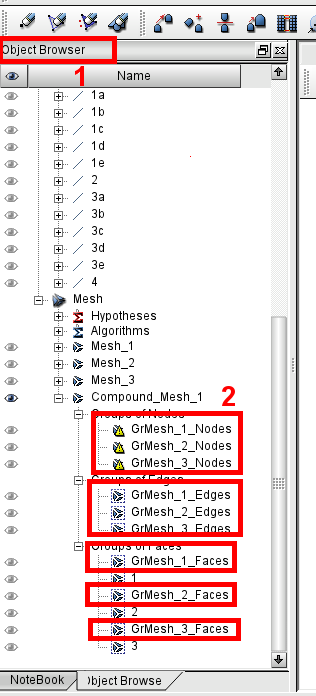
\includegraphics[scale=0.50]{figures/SalomeStep5b.png}
\caption{Deleting Unnecessary Groups.}
\label{fig:no3.2.1.15}
\end{center}
\end{figure}
          
The same technique as the above tip can be used to define the Boundary IDs by selecting them by hand. Another method that is easier for more complex shapes with finer meshes can be done as follows. Go back to \textbf{Geometry} and create lines around the Boundary. Like vertices this is done by going \textbf{New Entity} $\rightarrow$ \textbf{Basic} $\rightarrow$ \textbf{Line}. Change \textbf{Name} to whatever is easiest for you, I prefer to give them some name related to the Boundary ID they represent and use a letter afterwards if multiple lines represent the same Boundary ID. Select the vertices along the line, then select \textbf{Apply}. The vertice in Point 2 will then move to Point 1 and you can then continue this process in a clockwise or counter-clockwise direction. Once you reach the last line you can then select \textbf{Apply and Close} (Figure \ref{fig:no3.2.1.16}).
  
\begin{figure}[tbp]
\begin{center}
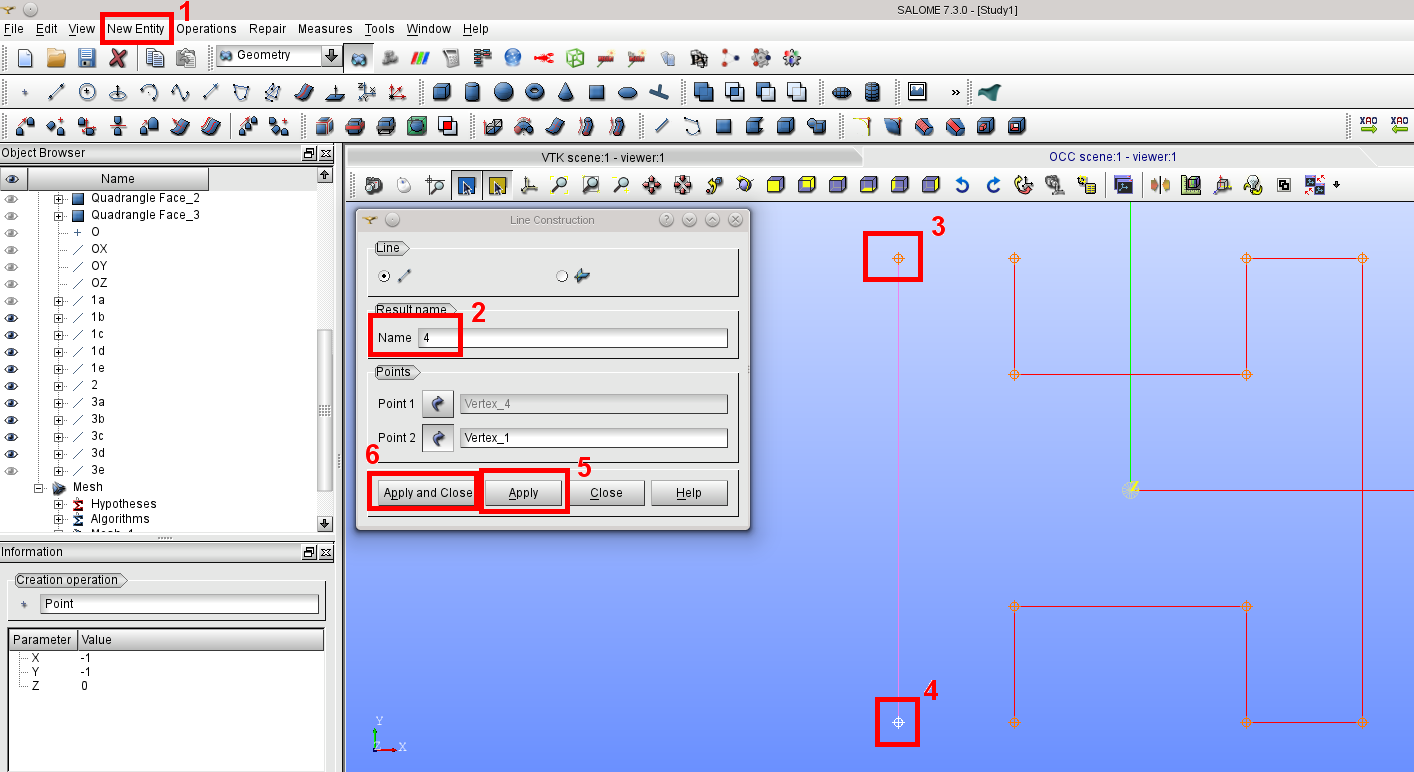
\includegraphics[scale=0.40]{figures/SalomeStep6.png}
\caption{Creating Lines for Use in Boundary ID Filter.}
\label{fig:no3.2.1.16}
\end{center}
\end{figure}

Back in \textbf{Mesh} right click the \textbf{Compound\_Mesh\_1} and select \textbf{Create Group}.  Select an \textbf{Element Type} of \textbf{Edge} and change the \textbf{Name} to the designated  Boundary ID. Select \textbf{Enable manual edition} and then select \textbf{Set Filter}.  In the case of Boundary ID 1 we have 5 lines so press \textbf{Add} 5 times then change   \textbf{Criterion} to \textbf{Belong to Geom}, \textbf{Binary} from \textbf{And} to \textbf{Or},  and for \textbf{Threshold value} select the empty square then select one of the lines from the  \textbf{Object Browser}. Once all the lines for the filter are set, select \textbf{Apply and Close}. Back in the \textbf{Create Group} window select \textbf{Add} and then \textbf{Apply and Close} (Figure \ref{fig:no3.2.1.17}). Repeat this process for each Boundary ID.
  
\begin{figure}[tbp]
\begin{center}
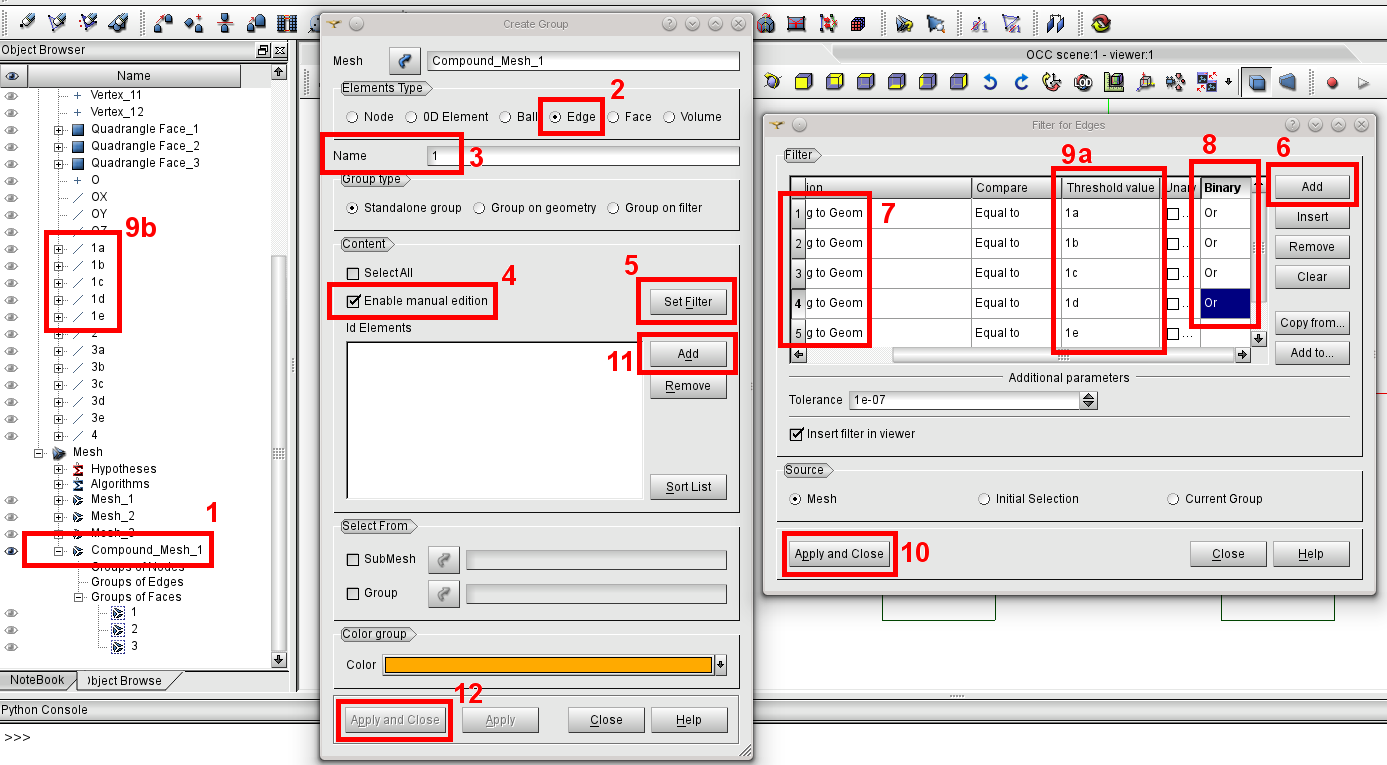
\includegraphics[scale=0.40]{figures/SalomeStep6b.png}
\caption{Creating a Boundary ID Filter.}
\label{fig:no3.2.1.17}
\end{center}
\end{figure}

\subsubsection{Removing internal edges}

Internal edges (and faces in 3D) are strictly prohibited by the OpenFCST architecture.  To see these internal edges, left click the Compound Mesh then right click the picture of it in the view. Then in \textbf{Numbering} select \textbf{Display Elements \#}. This will display all the edge and face numbers. As shown in Figure \ref{fig:no3.2.1.18}, it can be seen that lines 3, 4, 17, and 18 must be deleted. 
  
\begin{figure}[h]
\begin{center}
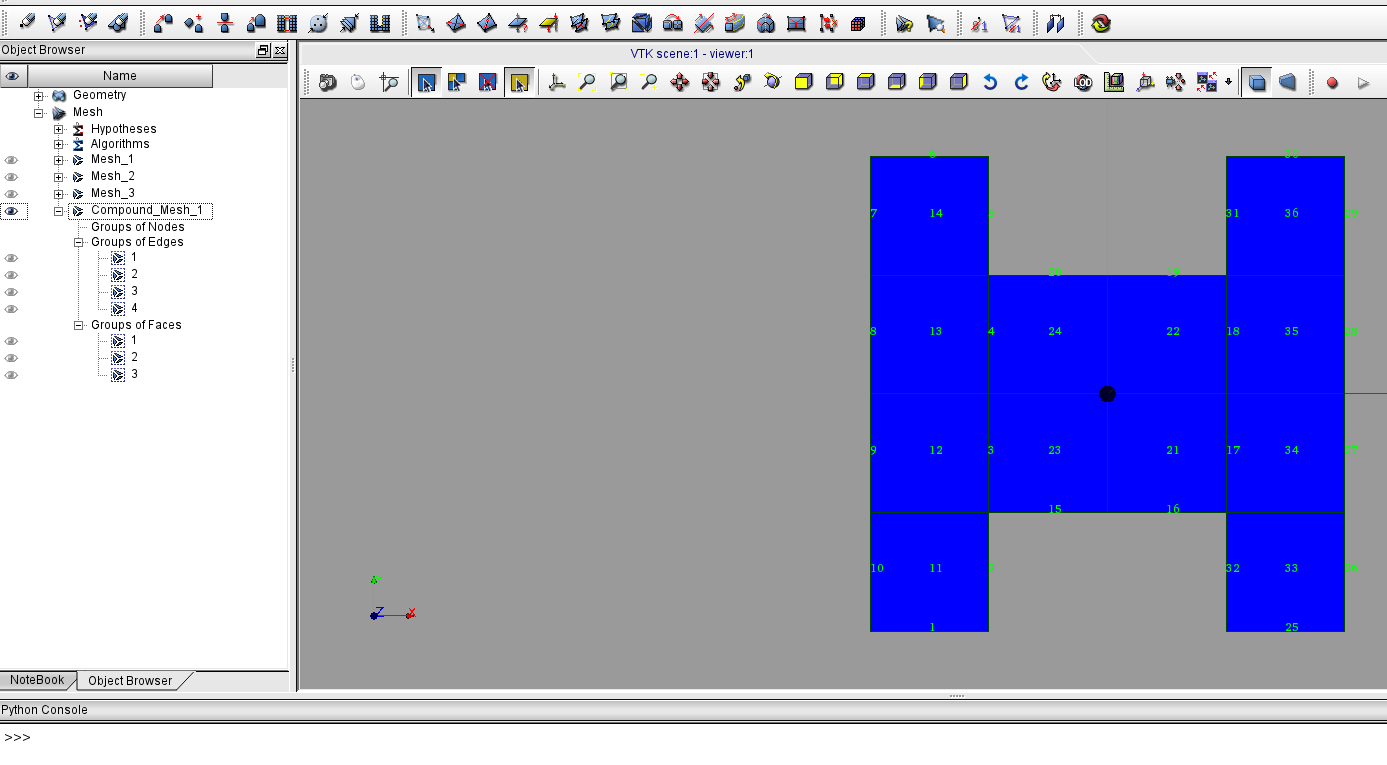
\includegraphics[scale=0.40]{figures/SalomeStep7.png}
\caption{Overview of the Mesh with Internal Edge Numbering (NOT allowed).}
\label{fig:no3.2.1.18}
\end{center}
\end{figure}
  
To manually remove these internal edges, in the toolbox select \textbf{Modification} $\rightarrow$ \textbf{Remove} $\rightarrow$ \textbf{Elements}. You can then either select the edge or enter the numbers and then select \textbf{Apply and Close}. This is rather easy in this simple project, but it can become cumbersome in more complex meshes. In openfcst/pre\_processing, there are two python scripts, RemoveInternalEdges.py and RemoveInternalFaces.py. In our case we need to open RemoveInternalEdges.py, change the mesh\_name on line 12 to the name of our Compound Mesh and save. Back in Salome select \textbf{File} $\rightarrow$ \textbf{Load Script} select the RemoveInternalEdges.py, and it will automatically remove all internal edges.
  
\subsubsection{Exporting the mesh to UNV format}

Now the mesh can be exported to a UNV file. Right click the Compound Mesh in the \textbf{Object Browser}, then select \textbf{Export} $\rightarrow$ \textbf{UNV file}. Finally, save your mesh. Once we export the whole mesh into an UNV file, we can use it for the computational purposes (see the respective OpenFCST tutorial).

\textit{Tip:} Sometimes issues are caused by the first few lines of the UNV file when importing it to OpenFCST. To prevent this you can delete the first 17 lines of the UNV file so the file actually begins at line 18. The begining of these UNV files all look similar to the following:

\begin{lstlisting}
    -1
   164
         1  SI: Meter (newton)         2
    1.0000000000000000E+0    1.0000000000000000E+0    1.0000000000000000E+0
    2.7314999999999998E+2
    -1
    -1
  2420
         1
SMESH_Mesh
         1         0         0
Global Cartesian Coordinate System
    1.0000000000000000E+0    0.0000000000000000E+0    0.0000000000000000E+0
    0.0000000000000000E+0    1.0000000000000000E+0    0.0000000000000000E+0
    0.0000000000000000E+0    0.0000000000000000E+0    1.0000000000000000E+0
    0.0000000000000000E+0    0.0000000000000000E+0    0.0000000000000000E+0
    -1
    -1
  2411
  ...
\end{lstlisting}
  
%%======================================================
\section{Salome meshing using python scripts}

%%=======
\subsection{Introduction}

The previous section discussed meshing in Salome using the graphical user interface (GUI). This section will focus on creating and running scripts to create meshes and geometries. Reasons for using scripts 
instead of the GUI are as follows: improved repeatability of results, significant time saving due to automation, and removal of human error. Several Python scripts included in the pre\_processing
folder can be used to create various meshes of various geometries.

Meshing scripts are run through Salomes text user interface (TUI). Loading scripts can be done simply via the File drop down menu, Load Script. Meshing scripts are written in Python programming language.
Python is a very popular general purpose high level programming language. Unlike C++, Python code is not precompiled, but interpreted at run time by a Python interpreter. Some key features
that make Python popular are its simple yet elegant syntax, dynamic typing, automatic memory management, and large selection of freely available libraries. If you are interested in
learning the Python programming language, we recommend \href{http://www.diveintopython.net/}{Dive Into Python}.

%%=======
\subsection{Scripting Examples}


\lstset{ %
language=Python,                % choose the language of the code
basicstyle=\footnotesize,       % the size of the fonts that are used for the code
numbers=left,                   % where to put the line-numbers
numberstyle=\footnotesize,      % the size of the fonts that are used for the line-numbers
stepnumber=1,                   % the step between two line-numbers. If it is 1 each line will be numbered
numbersep=5pt,                  % how far the line-numbers are from the code
backgroundcolor=\color{white},  % choose the background color. You must add \usepackage{color}
showspaces=false,               % show spaces adding particular underscores
showstringspaces=false,         % underline spaces within strings
showtabs=false,                 % show tabs within strings adding particular underscores
frame=single,           % adds a frame around the code
tabsize=2,          % sets default tabsize to 2 spaces
captionpos=b,           % sets the caption-position to bottom
breaklines=true,        % sets automatic line breaking
breakatwhitespace=false,    % sets if automatic breaks should only happen at whitespace
escapeinside={\%*}{*)}          % if you want to add a comment within your code
}


\begin{lstlisting}
import smesh, geompy, SMESH
import SALOMEDS   
\end{lstlisting}


The above lines import the necessary Salome packages that will be required to create geometries and meshes. \textit{smesh} is used to create python mesh objects,
\textit{geompy} is used for creating geometries. The other two packages contain constant flags. For more detail, please see the following resources:

\begin{enumerate}
 \item \href{http://docs.salome-platform.org/salome_6_5_0/gui/SMESH/smeshpy_doc/smesh_8py.html}{\textit{smesh} functions};
 \item \href{http://docs.salome-platform.org/salome_6_5_0/gui/GEOM/tui_basic_geom_objs_page.html}{\textit{geompy} documentation};
 \item \href{http://docs.salome-platform.org/salome_6_5_0/gui/SMESH/smeshpy_interface_page.html}{Salome TUI documentation}.
\end{enumerate}

The following simple example shows how to use geompy to create a simple geometry and then mesh it using smesh.

\begin{lstlisting}
def makeRectanglarMesh(self, width, height):

    #Create vertices to describe rectangle
    Vertex_1 = geompy.MakeVertex(dList[0], dList[1], dList[2])
    Vertex_2 = geompy.MakeVertex(dList[0] + width, dList[1], dList[2])
    Vertex_3 = geompy.MakeVertex(dList[0] + width, dList[1] + height, dList[2])
    Vertex_4 = geompy.MakeVertex(dList[0], dList[1] + height, dList[2])
    
    #Make rectangle geometries
    rect = geompy.MakeQuad4Vertices(Vertex_1, Vertex_2, Vertex_3, Vertex_4)
    
    #Create mesh object of rectangular geomtery
    Mesh_1 = smesh.Mesh(rect)
    
    #Set 1D meshing algorithm
    Regular_1D = Mesh_1.Segment()
    Local_Length_1 = Regular_1D.LocalLength(self.meshDensity)
    Local_Length_1.SetPrecision( 1e-07 )
    
    #Set 2D meshing algorithm
    Mesh_1.Quadrangle()
    
    #Compute and return
    Mesh_1.Compute()
    return Mesh_1 

\end{lstlisting}

The following is an example of modifying meshes and using mesh filters.

\begin{lstlisting}
def delInternalEdges(self):
    'This function deletes internal edges from self.compoundMesh'
    
    #Create a search filter to find free borders of the mesh
    search_filter = smesh.GetFilter(smesh.EDGE, smesh.FT_FreeBorders)
    external_edges = self.compoundMesh.GetIdsFromFilter(search_filter)
    
    #Get a list of all edges
    all_edges = self.compoundMesh.GetElementsByType(SMESH.EDGE)
    
    edges_to_remove = []
    
    #The difference between the external_edges list and all_edges list will be the internal edges.
    #The following loop iterates through the all_edges list, comparing it wil the external_edges list.
    
    for b in all_edges:
	if b in external_edges:
	    pass
	else:
	    #The edge is internal, add it to the list of items to be removed from the mesh
	    edge_to_remove.append(b)
    
    print "Removing internal edges:"
    print edges_to_remove
    
    #Remove the edges from the mesh
    self.compoundMesh.RemoveElements(edges_to_remove)
    
\end{lstlisting}        

When developing a new Python function for generating a geometry or mesh in Salome one may obtain a rough solution by following these steps:

\begin{enumerate}
 \item open the Salome GUI;
 \item perform the necessary steps using the GUI to generate the desired geometries and/or surfaces;
 \item use the ``Dump Study'' facility, accessed from the File menu, to produce a bulky but complete python program for the previously performed steps;
 \item refine the script to the desired form.
\end{enumerate}

This is a very good method for obtaining an initial coding solution or examples of correct code syntax and usage.


\lstset{ %
language=C++,                % choose the language of the code
basicstyle=\footnotesize,       % the size of the fonts that are used for the code
numbers=left,                   % where to put the line-numbers
numberstyle=\footnotesize,      % the size of the fonts that are used for the line-numbers
stepnumber=1,                   % the step between two line-numbers. If it is 1 each line will be numbered
numbersep=5pt,                  % how far the line-numbers are from the code
backgroundcolor=\color{white},  % choose the background color. You must add \usepackage{color}
showspaces=false,               % show spaces adding particular underscores
showstringspaces=false,         % underline spaces within strings
showtabs=false,                 % show tabs within strings adding particular underscores
frame=single,           % adds a frame around the code
tabsize=2,          % sets default tabsize to 2 spaces
captionpos=b,           % sets the caption-position to bottom
breaklines=true,        % sets automatic line breaking
breakatwhitespace=false,    % sets if automatic breaks should only happen at whitespace
escapeinside={\%*}{*)}          % if you want to add a comment within your code
}

%%===============================================================
%%===============================================================
%%===============================================================
%%===============================================================
\chapter{Running OpenFCST}
%%===============================================================
%%===============================================================
%%===============================================================
% Authors: M. Secanell, K. Domican, P. Wardlaw
%%===============================================================

%%==============
\section{Setting up a simulation in OpenFCST}

In order to setup a simulation in OpenFCST, either two or three parameter files are required. Note that the xml files are used with the graphical user interface (GUI) while prm files are used if you execute the program through terminal. The required files are:
\begin{enumerate}
 \item main.prm (or main.xml): This is the file that is first specified in the OpenFCST GUI. When calling OpenFCST from the command line, this is the only file passed as an argument. This file is used to specify the type of simulation/application that the user would like to run. The other files are constructed based on the options in this file.
 \item data.prm (or data.xml): This file contains all the information regarding the computational domain, boundary and operating conditions (\textit{Relative Humidity, Temperature, ...}), equations, solution strategies and post-processing options to solve the simulation. It also specifies all the parameters that describe the fuel cell physical properties (\textit{Porosity, Platinum \& Nafion Loading, ...}).
 \item opt.prm (or opt.xml): This file is used ONLY if in the main file section \texttt{Simulator}, subsection \texttt{Analysis type} is set to \texttt{Optimization}. The file is used to specify the required information to run an optimization simulation. Two optimization examples for cathode electrode are shown in the example folder.
\end{enumerate}
Sometimes we refer to these files as an OpenFCST project.

These files are used to specify the type of problem, and the fuel cell parameters necessary to run a simulation in OpenFCST. To run OpenFCST, either the GUI is used with the xml files or the program can be called from the command line (with the prm files) using the following command:
\begin{lstlisting}
$~/Openfcst/Install/bin/> ./fuel_cell-2d.bin main.prm
\end{lstlisting}
The main file already contains the path to the other files, so only this file is needed. Upon issuing this command OpenFCST will select the desired simulation to run, read the fuel cell parameters from the different files, and then solve the required finite element problem. The program flowchart is given in Figure \ref{analysis_schematic}. The output of the program is shown on screen and also recorded in a file, i.e., \texttt{logfile.log}.

\begin{figure}[h]
\begin{center}
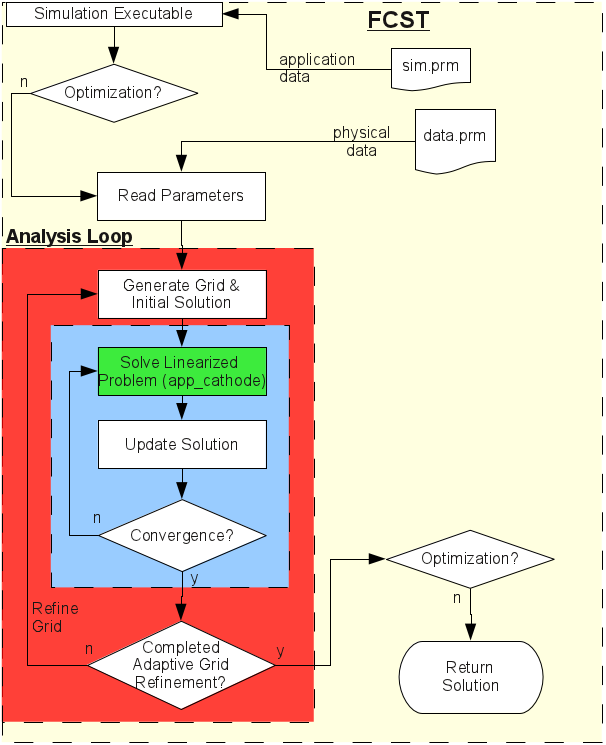
\includegraphics[width=0.5\textwidth]{figures/analysis_schematic.png}
\caption{Schematic of Fuel Cell Analysis Code.}
\label{analysis_schematic}
\end{center}
\end{figure}

In the next sections, first the OpenFCST graphical user interface is discussed. Then, the main and data files are discussed in detail. The files with extension .xml are read with the OpenFCST GUI. The files with extension .prm are ASCII files. The latter contain the same information, but they are easier to read in a text editor. OpenFCST can convert .prm files to .xml files easily. If you have a folder with a main.prm and a data.prm files (the data file name can be anything, but it must be specified in the main.prm file), then you can call OpenFCST as follows:
\begin{lstlisting}
$~/Openfcst/Install/bin/> ./fuel_cell-2d.bin -c main.prm
\end{lstlisting}
Then main and data files in XML format will be generated based on the main.prm file provided. The XML files can then be visualized and modified with the OpenFCST GUI.

%%==============
\section{OpenFCST examples}

The folder \texttt{examples} in the \texttt{Install} folder in OpenFCST contain an HTML manual with several examples. The examples are part of our testing suite to make sure that OpenFCST continues to provide the same results as new functionality is added. Each sub-directory in \texttt{examples} contains an explanation of the problem that is being solved as well as the data files to obtain the results. The easiest way to get started with OpenFCST is to run the example cases. We suggest that you do not modify the files in the examples folder, instead copy them to a different sub-folder such as \texttt{my\_data} so that you can still test your code with \texttt{run\_tests}.

The folder \texttt{examples/} contains .prm files. We recommend that you convert them to .xml files and then visualize them in the OpenFCST GUI. 

%%==============
\section{OpenFCST's graphical user interface}

%Purpose:
The OpenFCST graphical user interface (GUI) allows one to create, configure, and run simulations within a single application. All the OpenFCST simulation parameters are viewable and editable through the GUI. Using the GUI, one can browse through the hierarchy of parameters to edit numerous aspects of a simulation. Parameter descriptions are displayed by mousing over a parameter name. Once suitable simulation parameters have been selected, a simulation can be run from within the GUI. Simulation output such as text logging and a list of generated files are displayed within the GUI in a convenient manner.

One may create a new project, whereby default parameter files will be created in a step-by-step process. Alternatively, one can load an existing project. A project is made of two to three files:
\begin{itemize}
 \item \texttt{main.xml} contains the main selections for OpenFCST, such as the type of application, nonlinear solver, and type of study to be performed, i.e. one analysis run or a parametric analysis run.
 \item \texttt{data.xml} contains the parameters to setup the simulation for the selected application.
 \item \texttt{opt.xml} is an optional file used to setup parameters for optimization.
\end{itemize}
There files are discussed in more detail later in this guide.

Given the large number of parameters in a simulation, we recommend that new users start with a project from the \texttt{examples} directory since the step-by-step process requires an in-depth knowledge of the code. In order to generate a GUI project from the examples folder, go to an example folder such as \texttt{cathode/analysis}, and then generate the XML files from the parameter files using the OpenFCST:
\begin{lstlisting}
$~/Openfcst/Install/examples/cathode/analysis> fcst2D -c main.prm 
\end{lstlisting}

Using the \texttt{main.prm} file, the .xml files that constitute a project are generated. The following output will appear in the terminal:
\begin{lstlisting}
Parameters: main.prm
Creating converted main file in XML
YOU ARE CURRENTLY SOLVING A CATHODE MODEL
Application->DoF->BlockMatrix->OptimizationBlockMatrix
->FuelCellShop::Equation::NewFicksTransportEquation
->FuelCellShop::Equation::ElectronTransportEquation
->FuelCellShop::Equation::ProtonTransportEquation
->FuelCellShop::Equation::ReactionSourceTerms
->FuelCell::Application::AppCathode-2D
YOU ARE USING Newton3pp NEWTON SOLVER
Application->Copy->Newton3ppBase->->AdaptiveRefinement
Parameters: data.prm
Creating converted data file in XML
No opt file detected, skipping.
\end{lstlisting}
Then \texttt{main.xml} and \texttt{data.xml} files will be generated.
 
Once the files are generated, they can be loaded into the GUI.

%===============================
\subsection{Overview}

In order to start the OpenFCST GUI, go to the \texttt{/Install/bin} folder and run the executable \texttt{fcst\_gui}. The GUI will start by asking for the binary to be used to run the simulations. There are two possible files that can be used:
\begin{itemize}
 \item \texttt{fuel\_cell-2d.bin}
 \item \texttt{fuel\_cell-3d.bin}
\end{itemize}
Select the first executable to run two-dimensional simulations, e.g., cathode and MEA, and the second for three-dimensional simulations, e.g. \texttt{ohmic} application.

The main components of the GUI shown in Figure \ref{fig:GUI_overview} can be described as follows:
\definecolor{red}{RGB}{255,0,0}
\definecolor{pink}{RGB}{255,0,255}
\definecolor{yellow}{RGB}{200,255,0}
\definecolor{blue}{RGB}{0,0,255}
\definecolor{green}{RGB}{0,255,0}
\definecolor{grey}{RGB}{90,90,90}

\begin{itemize}
 \item \textbf{\textcolor{pink}{File menu:}} From this menu we can start a new project, open an existing project, save the current project, save a specific file from the current project, save the simulation log to a text file, and exit the GUI. 
 \item \textbf{\textcolor{red}{Parameter editing panel:} } This panel displays all the parameters of the loaded project. We can browse through the parameter hierarchy using the mouse to locate the parameter we desire. Descriptions/hints about a specific parameter are displayed by mousing over it.
 \item \textbf{\textcolor{yellow}{Start/next/end button:}} This button is used predominantly to progress our current project.
 \item \textbf{\textcolor{green}{Application Output:} } While running a simulation, text output describing the status of the simulation will be shown here.
 \item \textbf{\textcolor{blue}{Output Files:}} While running a simulation, OpenFCST will produce several output files. Clicking on any item displayed in this list will open the file with the operating system default program associated to the file's type. 
\end{itemize}

\begin{figure}[tbp]
\begin{center} 
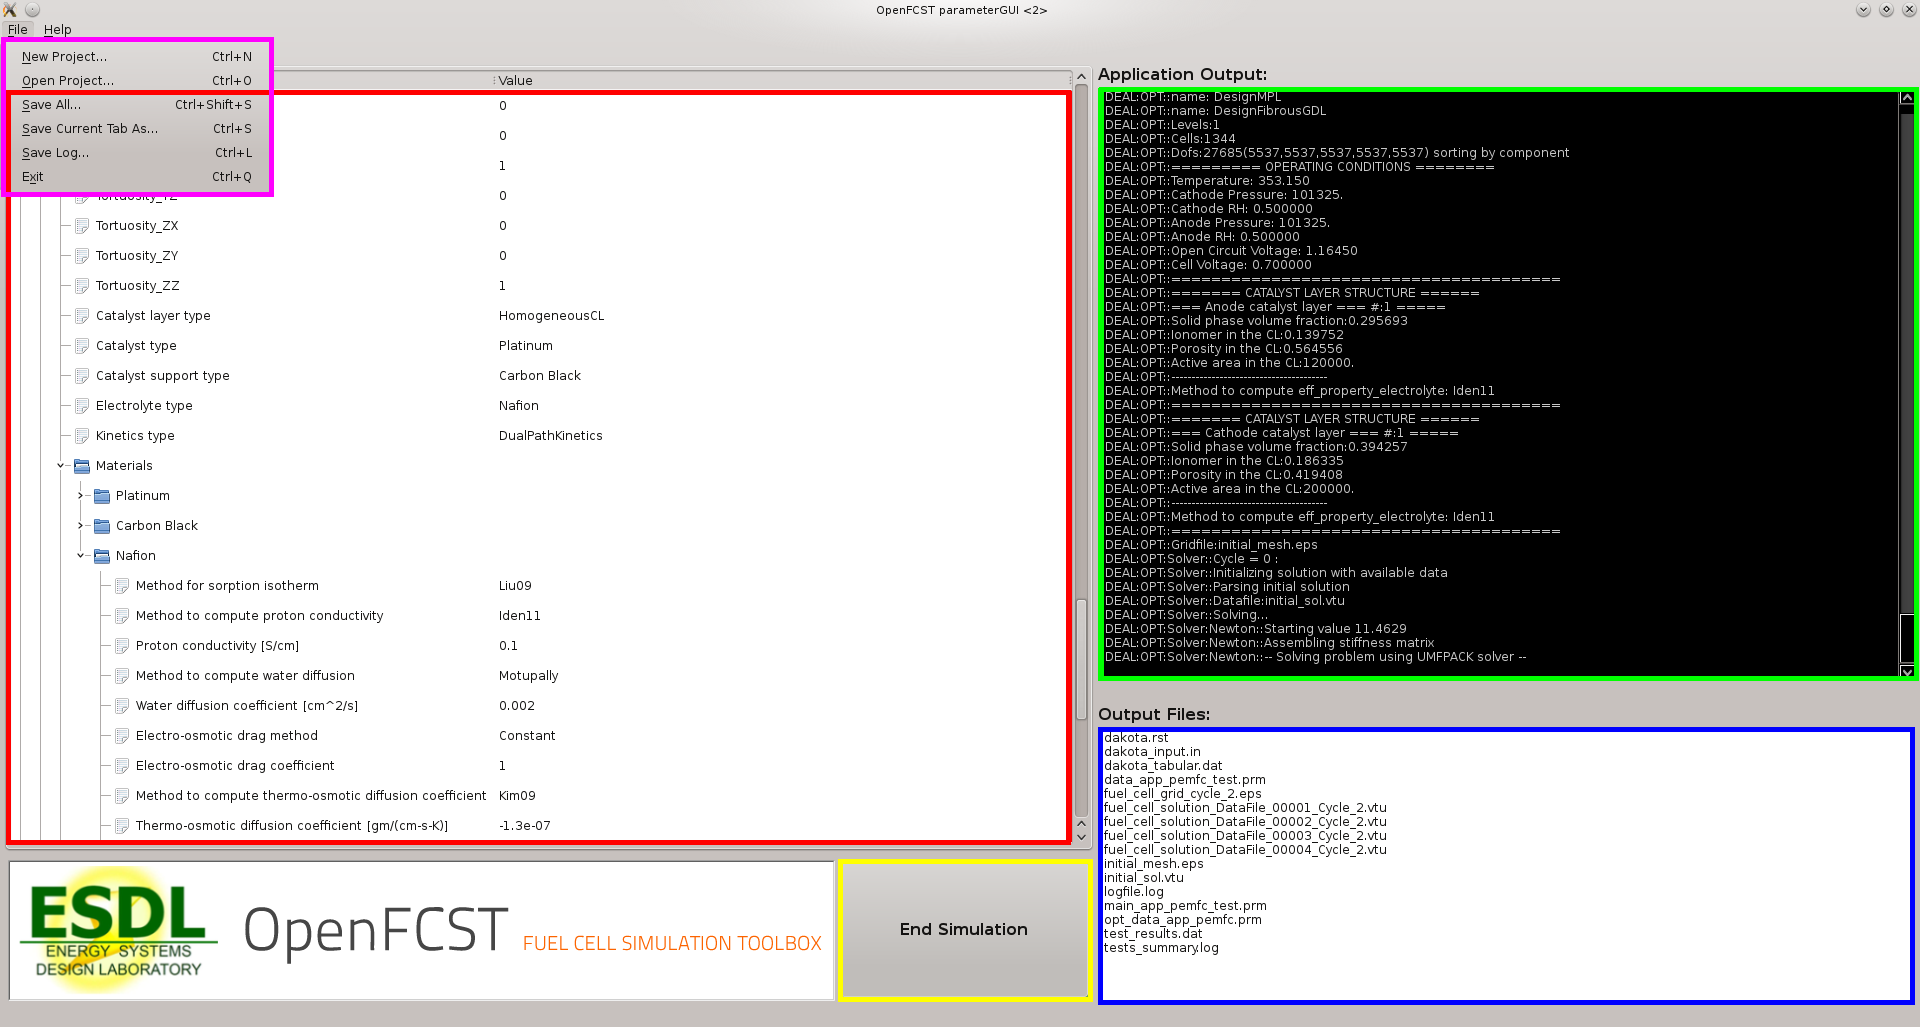
\includegraphics[width=\textwidth]{./figures/gui2.png}
\caption{Main window of the OpenFCST graphical user interface. Components of interest are highlighted.}
\label{fig:GUI_overview}
\end{center}
\end{figure}

%===============================
\subsection{How To's}
%---
\subsubsection{Start a New Project} \label{sec:start_new_project_gui}
\textcolor{red}{Warning:} Default parameter files created by OpenFCST version 0.2 require extensive modification in order to run a simulation. We suggest that users new to OpenFCST use the ``Open Project'' option explained later in this section.

Starting a new project from scratch using the GUI is simple:

\begin{enumerate}
 \item First, select the ``New Project'' option from the \textcolor{pink}{file menu}.
 \item A dialogue will open asking you to select a folder, i.e. a ``working directory''. This is the location  where your project file and simulation output will be placed. \textcolor{red}{Warning:} placing a project in a folder with an existing project may cause some files to be overwritten.
 \item Once a working directory has been selected, OpenFCST will generate a main parameter file. This file allows us to select important aspects of our simulation, such as the type of application we would like to run (Cathode simulation, non-isothermal application, etc) and the type of Newton solver we would like to use.
 \item At this point, clicking the \textcolor{yellow}{Next} button will instruct OpenFCST to read our main file and generate a corresponding data file. A data file includes important parameters pertaining to simulation aspects such as equations,  finite elements,  mesh refinement, and fuel cell material parameters. Additionally, an optimization file may be generated, depending on if you have compiled OpenFCST with Dakota.
 \item Now that we have edited our parameter files to our desire, clicking the \textcolor{yellow}{Run} button will start the simulation. Whilst the simulation is running, its status will be shown by the \textcolor{green}{Application Output panel} and a list of files generated by OpenFCST will be shown in the \textcolor{blue}{Output File panel}.
 \item If there are no errors, the simulation will run to completion.
\end{enumerate}

%---
\subsubsection{Open an Existing Project}\label{sec:open_existing_project_gui}
Opening an existing project using the GUI is a simple process, similar to starting a new one.

\begin{enumerate}
 \item Select ``Open Project'' from  the \textcolor{pink}{file menu}.
 \item You will be asked to specify the location of a \textbf{main} parameter file. \emph{Note:} The directory of the main file will be used as the project\textquoteright s working directory, i.e. the location where your project files and simulation output will be placed. 
 \item Once the location of the main file has been specified, you will be asked for the location of the \textbf{data} file.
 \item Once the location of the data file has been set, you can load additional files, such as optimization parameter files. It is not necessary to load these additional files. 
 \item Now you can edit the loaded files and run the simulation by clicking the \textcolor{yellow}{run} button, in the same fashion as described earlier in this section.
\end{enumerate}

%---
\subsection{Configuration}
The version of the OpenFCST binary you are using may have unique interface arguments. To maintain functionality between the GUI and the OpenFCST binary the following parameters are editable in the GUI's \textbf{settings.ini} file (which will be created in the same directory as the GUI once it is run). Typically,  these parameters do not need to be edited.

\begin{itemize}
 \item \textcolor{grey}{\textbf{OpenFCSTbin:}} The path to the OpenFCST binary you wish to use to run your simulations.
 \item \textcolor{grey}{\textbf{OpenFCSTparamArg:}} The command line argument which instructs OpenFCST to create a parameter file.
 \item \textcolor{grey}{\textbf{mainFileName:}} The name of the main file OpenFCST will create when generating a new Project.
 \item \textcolor{grey}{\textbf{dataFileName:}} The name of the data file which OpenFCST will create when generating a new Project.
 \item \textcolor{grey}{\textbf{optFileName:}} The name of the optimization file which OpenFCST will create when generating a new Project.
\end{itemize}

%---
\subsection{Reporting Errors}
In the case of program errors or crashes occurring,  please \htmladdnormallink{contact us}{http://www.esdlab.mece.ualberta.ca/contact.php}. 

Providing the following  will help us to resolve your issue:

\begin{itemize}
 \item a description of the circumstances in which the errors occurred and any error messages that you may have received;
 \item a copy of your parameter files (main.xml, data.xml, etc);
 \item the GUI log file (gui\_log.txt);
 \item simulation log files (which can be produced using the graphical user interface, and found in the project's working directory).
\end{itemize}

%%==============
%%==============
\section{The OpenFCST \texttt{main} file}

The \texttt{main} file is the initial file accessed by OpenFCST. The file contains two main subsections:
\begin{enumerate}
 \item \texttt{Simulator};
 \item \texttt{Logfile}.
\end{enumerate}

%-----
\subsection{\texttt{Simulator} section}
The \texttt{Simulator} section is used to setup the high-level parameters for the simulation such as the application to solve, the type of solver, and the type of results. This section is maybe the most important as it dictates the information that will appear in the data file for the GUI. Please note that some parameters cannot be modified once the data file has been generated. The parameters in this section are:
\begin{itemize}
 \item \texttt{simulator name}: This entry specifies the type of simulation that you would like to perform, e.g., solve a cathode model (\texttt{cathode}), a full MEA model (\texttt{MEA}), an electrical conduction problem (\texttt{ohmic}). The data file is dependent on the selection of this parameter, therefore, if the default data file is generated with one value, it will not work with others.
 \item \texttt{simulator specification}: This entry is only used with fluid flow applications to specify different sub-problems based on boundary conditions.
 \item \texttt{solver name}: This entry specifies if the problem is linear (Linear) or non-linear. For the latter, the OpenFCST team has implemented several Newton solvers that can be used. Note that the data file should be re-generated if the type of solver is changed.
 \item \texttt{solver method}: This entry can be used to add an additional loop during the solution stage after the analysis loop (see Figure~\ref{analysis_schematic}).
 \item \texttt{simulator parameter file name}: This entry should contain the name of the data file for the simulation. The data file should be in the same folder as the main file.
 \item \texttt{Analysis type}: This entry specifies if you would like to run a simulation for a specific cell operating condition, a polarization curve, a parametric study, or an optimization case. The options for each one of these cases are specified in the later subsections. For \texttt{Analysis}, no further information is required. For the other cases, the necessary information is specified next.
\end{itemize}

Subsections \texttt{Optimization}, \texttt{Parametric Study} and \texttt{Polarization Curve} are described next. For \texttt{Polarization Curve}, the following parameters can be specified:
\begin{itemize}
  \item \texttt{Polarization curve file output}: This entry specifies the file where the polarization curve results should be stored;
  \item \texttt{Initial voltage [V]}: Voltage at which the first point in the polarization curve will be evaluated;
  \item \texttt{Final voltage [V]}: Voltage at which the polarization curve will be terminated. Note that if the value is set, for example, to 0.6 V, then the polarization curve will not include this voltage (it will run down to 0.6~V plus increment);
  \item \texttt{Increment [V]}: Spacing between points in the polarization curve;
  \item \texttt{Adaptive Increment}: Set to true if you would like to reduce the voltage increment adaptively if convergence could not be achieved with the larger value;
  \item \texttt{Min. Increment [V]}: If Adaptive Increment is set to true, this value controls the minimum change in cell voltage before the polarization fails to converge and the voltage is updated again. Note that this value has to be positive as a value of zero would lead to an infinite loop.
\end{itemize}

Subsection \texttt{Parametric Study} is used when a parametric study is to be performed for a different variable than cell voltage. In this case, the most important parameter to specify is \texttt{Parameter name} which identifies the parameter that is to be modified. Any parameter in the OpenFCST data file can be modified following the format specified below. The parameters and how to modified are explained below:
\begin{itemize}
 \item \texttt{Parameter file output}: File where the parametric study results should be stored.
 \item \texttt{Parameter name}: Enter the name of the parameter you would like to study. Use one of the following formats:
 \begin{itemize}
   \item For normal parameter: \texttt{Subsection\_1$>>$Subsection\_2$>>$Value};
   \item For boundary value or graded: \texttt{Subsection\_1$>>$Subsection\_2$>>$Material\_id:Value},
 \end{itemize}
   where \texttt{Subsection\_1} and \texttt{Subsection\_2} would be the sections where the parameter is found in the data file. For example, if we would like to change the temperature of the cell, we would write \texttt{Fuel cell data$>>$Operating conditions$>>$Temperature cell}.
   \item \texttt{Initial value}: Enter the value you would like to start the parametric study from.
   \item \texttt{Final value}: Enter the final value for the parametric study.
   \item \texttt{Increment}: Spacing between points in the parametric study.
   \item \texttt{Adaptive Increment}: Set to true if you would like to reduce the increment adaptively if convergence could not be achieved with the larger value
   \item \texttt{Min. Increment}: If Adaptive Increment is set to true, this value controls the minimum change in parameter before the polarization fails to converge and the voltage is updated. Note that this value has to be positive as a value of zero would lead to an infinite loop.
   \item \texttt{Parameter values}: If you would like to run the parametric study for only some points, then a list containing the discrete values of a parameter of study can be included here. If this value is empty, then the Initial and Final value entries are used, if this list is filled, then the list is used instead.
\end{itemize}

Subsection \texttt{Optimization} is used when an optimization study is to be performed. In this case, the file that includes all optimization parameters is to be included here. There are only two entries in this subsection:
\begin{itemize}
 \item \texttt{optimization parameter file name}: Enter here the name of the optimization file. By default, if using the GUI, opt.xml should be used.
 \item \texttt{Dakota direct}: Set to true if you would like OpenFCST to directly interact with Dakota, i.e. OpenFCST will call Dakota as needed to run the optimization simulation. If set to false, then OpenFCST will run once and output a file that Dakota can read. In this case Dakota would be the optimization driver.
\end{itemize}

\subsection{The \texttt{Logfile} section}
The \texttt{Logfile} section is used to specify where the output from OpenFCST should be stored and how much output should be stored.

%%==============
\section{The OpenFCST \texttt{data} file}

The OpenFCST data file will change depending on the parameters that are specified in the main file, but in general it contains the following sections:
\begin{itemize}
 \item \texttt{Adaptive refinement}: This section is used to control adaptive refinement options. Only advanced users should modify this section.
 \item \texttt{Newton}: Section used to specify the parameters that control the Newton solver to solve the problem.
 \item \texttt{Grid generation}: Section used to specify the geometry of the domain. \textbf{This section is critical} as the ID specified in this section for \texttt{material\_ID} and \texttt{boundary\_ID} are used to impose the appropriate initial and boundary solution in section Equations. 
 \item \texttt{Discretization}: This section is used to specify the type of finite element used to discretize the governing equations. The quadrature formula and degree are also set here.
 \item \texttt{System management}: This section is used to specify the equations that need to be solved. In most cases, this section is filled automatically by the application.
 \item \texttt{Equations}: \textbf{This section is critical}. In this section, the initial solution and boundary conditions for each equation need to be specified. The values are specified using the following format \texttt{material\_ID}:value and \texttt{boundary\_ID}:value. This section will be discussed below in more detail.
 \item \texttt{Reaction source terms}: This section is used to turn on/off source terms for the equations.
 \item \texttt{Initial Solution}: This section is used to control initialization and output of the initial solution. OpenFCST can generate a default initial solution or a previous solution can be used as an initial guess. This section allows users to create an initial solution for later use and to load previous solutions as an initial solution. Note that the initial and final solution have to be on the same mesh. OpenFCST also allows users to output the initial solution here.
 \item \texttt{Linear Solver}: This section is used to select the linear solver that users want to use. Several direct and iterative solvers are available. For non-linear problems, only direct solvers, e.g., \texttt{UMFPACK} and \texttt{MUMPS}, and iterative solver ILU-GMRES are satisfactory due to the nature of the Jacobian matrix to be inverted. 
 \item \texttt{Fuel cell data}: This is the most important section of OpenFCST for a user as it encapsulates all the fuel cell information, e.g., operating conditions, type of kinetic model, catalyst layer model and GDL type.
 \item \texttt{Output}: This subsection is used to specify the output format for the mesh and the output solution data. In general, we recommend EPS and VTU formats for grid and data respectively. Only advanced users should modify this section.
 \item \texttt{Output Variables}: This section is used to request OpenFCST to calculate and output a variety of functionals, i.e., integral quantities, at postprocessing such as current density and water crossover.
 \item \texttt{Postprocessing}: This section is used in order to provide additional information to compute the functionals specified in \texttt{Output Variables}.
\end{itemize}

%---
\subsection{The \texttt{Adaptive refinement} section}

This section is used in combination with the flags in \texttt{Grid generation} section to control refinement levels and output options for the mesh and solution. 

This section has the following entries:
\begin{itemize}
 \item \texttt{Number of Refinements}: This parameter is used to define the number of times the mesh will be refined. The minimum value is one, i.e., only the original mesh is solved. At each adaptive refinement level, either all the cells (global) or 30\% of the cells with largest error (computed using an error estimator; adaptive) are split into four. The process is repeated at each refinement level. An example of mesh that is refined globally several times and an adaptively refined mesh is shown in Figure \ref{fig:grid_adaptive_refinement}.
   \item  \texttt{Refinement}: This flag specifies the type of refinement to be used if in \texttt{Adaptive refinement} section you decided to solve the problem in several meshes. Mainly two options are available:
  \begin{enumerate}
   \item global: At each refinement level, each cell in the domain is divided into four new cells.
   \item adaptive: At each refinement level, a percentage, specified in texttt{Refinement threshold}, of cells with the largest error are divided into four cells. Also, the percentage of cells in \texttt{Coarsening threshold} with the smallest error are re-merged into one cell if they had been previously refined. 
  \end{enumerate}
 \item \texttt{Refinement threshold}: For adaptive refinement, the percentage of cells with largest error that should be refined.
 \item \texttt{Coarsening threshold}: For adaptive refinement, the percentage of cells with smallest error that should be coarsened.
 \item \texttt{Output initial mesh}: Set flag to true if you want to output an EPS figure of the initial mesh using the value in \texttt{Output initial mesh filename}.
 \item \texttt{Output initial mesh filename}: Filename of where the initial mesh will be output.
 \item \texttt{Output intermediate solutions}: Set flag to true if you would like the solution at each grid refinement to be output. Please note that outputting the solution is time consuming.
 \item \texttt{Output intermediate responses}: Compute the functionals in \texttt{Output variables} at each grid refinement. Use this option if you want to perform a grid refinement study. Please note however that computing the functionals is time consuming.
 \item \texttt{Output final solution}: Output the final solution to a file.
 \item \texttt{Compute errors and convergence rates}: Internal option for developers. Always set this value to false.
 \item \texttt{Use nonlinear solver for linear problem}: Internal option for developers. Always set this value to false.
\end{itemize}

\begin{figure}[tbp]
\centering
\minipage{0.2\textwidth}
  
\includegraphics[width=\linewidth]{figures/grid_no_refinement.png}
  \caption{Initial Grid.}
\endminipage\hfill
\minipage{0.2\textwidth}
  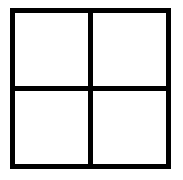
\includegraphics[width=\linewidth]{figures/grid_first_refinement.png}
  \caption{Global $1^{st}$ Refinement.}
\endminipage\hfill
\minipage{0.2\textwidth}
  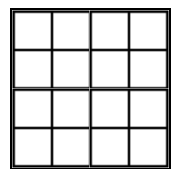
\includegraphics[width=\linewidth]{figures/grid_second_refinement.png}
  \caption{Global $2^{nd}$ Refinement.}
\endminipage\hfill
\minipage{0.2\textwidth}
  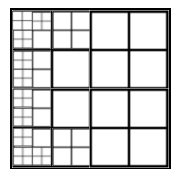
\includegraphics[width=\linewidth]{figures/grid_adaptive_refinement.png}
  \caption{Adaptive Refinement.}
  \label{fig:grid_adaptive_refinement}
\endminipage\hfill
\end{figure}


In order to control the type of refinement, \texttt{Grid generation>>Refinement} is used. This value can be set to adaptive or global in order to specify the type of refinement. Furthermore, if adaptive is used, the percentage of cells that are refined and coarsened is given by \texttt{Grid generation>>Refinement threshold} and \texttt{Grid generation>>Coarsening threshold}.

%---
%---
\subsection{The \texttt{Newton} section}

This section specifies the parameters that are used to control the Newton iteration for the case of non-linear problems. There are many parameters most of which are self-explanatory. The most critical parameters are:
\begin{itemize}
 \item \texttt{Max steps}: Used to limit the number of iterations carried out by the Newton solver.
 \item \texttt{Tolerance}: The value of the L${}^2$-norm of the residual. Ideally, this tolerance should be kept at $1.0e^{-9}$. However, in certain circumstances, convergence with that tolerance may not be possible or feasible given the computational time. In these scenarios it is possible to reduce the tolerance to $1.0e^{-4} - 1.0e^{-6}$ while still keeping reasonable accuracy.
 \item \texttt{Reduction}: Use if you want convergence to be accomplished after the initial residual (or whatever criterion was chosen by the solver class) is reduced by a given factor. This is useful in cases where you don't want to solve exactly, but rather want to reduce the residual by a small amount. We recommend setting this value always to $1.0e^{-20}$.
\end{itemize}

In order to control the solution output during the Newton iteration, the following four parameters can be used
\begin{itemize}
 \item \texttt{Debug level}: Write debug output to the logfile. The higher the number, the more output. The range is between 0 and 3.
 \item \texttt{Debug residual}: Output the residual at every Newton iteration. This then can be used to locate errors/bugs in the code.
 \item \texttt{Debug solution}: Output the solution at every Newton iteration. This then can be used to locate errors/bugs in the code.
 \item \texttt{Debug update}: Output the solution update at every Newton iteration. This then can be used to locate errors/bugs in the code.
\end{itemize}

The parameters \texttt{special\_block\_i} are internal variables. They should not be used by the users.

%---
%---
\subsection{The \texttt{Grid generation} section}

The \texttt{Grid generation} section is one of the most important sections in OpenFCST, together with the \texttt{Fuel cell data} section. This section is used to define the geometry for the fuel cell. The fuel cell geometry is represented by the following data:
\begin{itemize}
 \item Length of each fuel cell layer, channel, and land.
 \item A collection of \texttt{Material ID}s used to identify each layer in the domain to the layers in the \texttt{Fuel cell data} section.
 \item A collection of \texttt{Boundary ID}s used to identify the boundaries of the domain where boundary conditions are applied.
\end{itemize}
These sections are key and are used in the \texttt{Equations} section to specify initial solution and boundary conditions and in \texttt{Fuel cell data} to associate each layer in the geometrical domain with the corresponding fuel cell properties.

The \texttt{Grid generation} section contains many entries. The following entries are used to specify the type of mesh and if any refinement on the mesh should be performed prior to the simulation:
\begin{itemize}
 \item \texttt{Type of mesh}: This entry specifies the type of mesh you would like to generate. You have two main options \texttt{ExternalMesh} will load an external mesh for your simulation. The other options use OpenFCST internal mesh generator to directly generate the geometry. 
 \item \texttt{File name}: If type of mesh has been set to \texttt{ExternalMesh}, this section should contain the name of the mesh file you would like to load. The file should be in the same folder as main.
 \item \texttt{File type}: Specify the extension of the file.
 \item \texttt{Initial refinement}: Number of times we want to globally refine the original grid before starting to solve.        
\end{itemize}

The following option is used to specify the numbering scheme for the degrees of freedom in the mesh. By default, degrees of freedom (DoFs) are sorted by component, but the following flag can be used to sort the DoFs using other schemes
\begin{itemize}
 \item \texttt{Sort Cuthill-McKee}: Organize the degree of freedom numbering for the mesh using the Cuthill-McKee algorithm.
\end{itemize}

The subsection \texttt{Internal mesh generator parameters} is only needed if the OpenFCST internal mesh generator is used. If it is not used, the section can be almost entirely ignored since the \texttt{ExternalMesh} should already contain material and boundary IDs. Some post-processing routines however might use several entries such as \texttt{Cathode CL thickness [cm]} and \texttt{boundary IDs}, so it might be necessary to fill out these values even if using an \texttt{ExternalMesh} in some instances.

The Dimensions subsection in \texttt{Internal mesh generator parameters} is used to specify the dimensions of each parameter in the cell. It contains the following:
\begin{itemize}
  \item \texttt{Cathode current collector width [cm]}: Thickness of the ribs of the bipolar plates (BPP) [cm].
  \item \texttt{Cathode channel width [cm]}: Thickness of the channels on the BPP [cm].
  \item \texttt{Cathode CL thickness [cm]}: Thickness of the cathode catalyst layer [cm].
  \item \texttt{Cathode GDL thickness [cm]}: Thickness of the cathode gas diffusion layer [cm].
  \item \texttt{Cathode MPL thickness [cm]}: Thickness of the cathode microporous layer [cm].
  \item For the remaining entries, please mouse over the entry in the GUI for meaning.
\end{itemize}

Subsection \texttt{Mesh refinement parameters}:
\begin{itemize}
  \item \texttt{Initial vertical cell count}: Number of cells we want in the y-direction of the original grid before starting to solve
  \item \texttt{Horizontal division of cathode GDL}: Number of cells we want in x-direction in the cathode GDL layer
  \item \texttt{Horizontal division of cathode CL}: Number of cells we want horizontally in the cathode CL layer
  \item For the remaining entries, please hover the mouse over the entry in the GUI for its meaning.
\end{itemize}

Subsection \texttt{Material ID} is used to define the material ID for each component of the cell. The material ID is used in \texttt{Fuel cell data} to associate each one of the cells in the mesh with the desired fuel cell properties. The entries in this section look as follows:
\begin{itemize}
  \item \texttt{Test}: Material ID for GridTest.
  \item \texttt{Cathode current collector}: Current collector material\_id.
  \item \texttt{Cathode gas channel}: Cathode gas channel material\_id.
  \item \texttt{Cathode GDL}: Cathode gas diffusion layer material\_id.
  \item \texttt{Cathode MPL}: Cathode microporous layer material\_id.
  \item For the remaining entries, please hover the mouse over the entry in the GUI for its meaning.
\end{itemize}

Subsection \texttt{Boundary ID} is used to define the boundary ID for each boundary in a fuel cell. These IDs are used in Equations section to specify Dirichlet and Neumann boundary conditions for each equation at each one of the defined boundaries. \textbf{The number 255 defines an interior boundary condition in deal.II. All internal boundaries MUST have a 255 boundary ID.} The entries in this section appear as follows:
\begin{itemize}             
  \item \texttt{c\_Ch/GDL}: Cathode gas channel and gas diffusion layer boundary\_id. 
  \item \texttt{c\_BPP/GDL}: Cathode bipolar plates and gas diffusion layer boundary\_id.
  \item \texttt{c\_GDL/CL}: Cathode gas diffusion layer and catalyst layer boundary\_id. Since this boundary is an internal boundary in most cases, it must be set to 255.
  \item For the remaining entries, please mouse over the entry in the GUI for meaning.
\end{itemize}

%--------------------
\subsection{The \texttt{Discretization} section}

The \texttt{Discretization} section is used to select the finite element discretization and the quadrature formula used to evaluate the weak form integrals. The key parameters defined in the subsection are:
\begin{enumerate}
\item \texttt{Element}: Defines the finite element discretization for each equation. This parameter is discussed in detail below.
\item \texttt{Degree Mapping}: Defines the geometric mapping. In most cases a linear mapping is used, i.e. set the value to 1.
\item \texttt{Boundary fluxes}: Set to true if there are any either Neumann or Robin boundary conditions. If the parameter is set to false, then OpenFCST will skip looping over boundaries resulting in faster computational speeds.
\item \texttt{Interior fluxes}: Set to true if there are any flux jumps between elements. This will only occur if using a Discontinuous Galerkin (DG) formulation. So far we have not implemented any DG schemes in OpenFCST.
\item \texttt{Matrix}: Used to control the number of quadrature points required to evaluate the integrals on the left hand side of the local weak form defining the partial differential equation. 
\item \texttt{Residual}: Used to control the number of quadrature points required to evaluate the integrals on the right hand side of the local weak form defining the partial differential equation. 
\end{enumerate}

Of the above parameters, \texttt{Element} is of critical importance as it specifies the type of finite element used for the spatial discretization. If only one equation is used, the element is specified as:
\begin{lstlisting}
  set Element = FE_Q(2)
\end{lstlisting}
where $FE\_Q(2)$ refers to the type of element, i.e. Lagrange element ($FE\_Q$), and the number in parenthesis, i.e, 2, is the order of the element, in this case quadratic. 

For system of equations, the finite element discretization for each equation needs to be specified. For example, for a system of five equations we would write
\begin{lstlisting}
  set Element = FESystem[FE_Q(2)^5] 
\end{lstlisting}
where FE\_Q(2) refers to the type of element and the number five in FE\_Q(2)\string^5 refers to the number of variables included in the quadratic category. If we want to use different elements for different variables we would specify it by separating the elements with a dash. For example, if we wanted the first two elements solved with a cubic Lagrange element and the last three solved with a linear Lagrange element approximation, we would insert the following line. FESystem[FE\_Q(3)\string^2-FE\_Q(1)\string^3]

The final two sections in \texttt{Discretization}, are
\begin{enumerate}
\item \texttt{Matrix};
\item \texttt{Residual}.
\end{enumerate}
Matrix and Residual control the number of quadrature points required to evaluate the integrals in the local weak form of our partial differential equation. The default value of -1 will set the number of quadrature points to the order of the finite element used plus one in each direction, e.g., for second order elements, number of quadrature points in each direction is $2 + 1 = 3$ (in 2D, using quadratic elements, the number of quadrature points would be 9). Assigning a default value of $-1$, for most cases, should be sufficient to achieve an exact solution of the integrals.

%--------------------
\subsection{The \texttt{System management} section}

The \texttt{System management} subsection is responsible for defining the \texttt{Solution variables} \&  \texttt{Equations} being used. This section is populated by the application directly and should not be modified by the users.

%--------------------
\subsection{The \texttt{Equations} section}

This section is responsible for specifying the initial solution and boundary conditions for the application at hand. The section is subdivided in one subsection per equation that needs to be solved. Inside each subsection, the main section needs to be specified:
\begin{itemize}
 \item \texttt{Initial data}: It is used to specify a piece-wise initial solution for the simulation. It contains two main entries:
 \begin{itemize}
  \item \texttt{Variable initial data}: If set to true and the application has implemented a variable initial guess, the variable initial guess is used.
  \item \texttt{variable\_name}: The name of this section corresponds to the variable we are trying to initialize. In this section, for each material ID a value needs to be given in order to setup an initial solution. The initial solution might be overwritten using the section \texttt{Fuel cell data>>Operating conditions}, however the map of material ID must be included here. If you have a mesh with two material IDs, e.g. CL is 5 and GDL is 8, and you would like to setup the initial solution for your variable to 0.2 and 0.3 in CL and GDL respectively, then the entry will be: \texttt{5:0.2, 8:0.3}. For each solution variable we have a comma-separated list of material ID, colon, value. 
 \end{itemize}
 \item \texttt{Boundary conditions}: Provides the ID for the type of boundary condition that you would like to have.
 \item \texttt{Boundary data}: Provides the value for Dirichlet, Neumann and Robin boundary conditions. As for the case of \texttt{Initial data}, the same format is used. Again this section is mandatory and it is the user's responsibility to create the appropriate map.
\end{itemize}

%--------------------
\subsection{The \texttt{Reaction source terms} section}
This section is used to turn on/off source terms for the equations.

%--------------------
\subsection{The \texttt{Initial Solution} section}

This section is used to control the initial guess that the user would like to use. As specified in \texttt{Equations}, a piece-wise approximation can be used as an initial guess. Another possibility is to use a previous solution as an initial guess. In this case, simulation is run first with the `\texttt{Output solution for transfer}' option set to true. This will produce a hidden file containing the solution. This solution can then be read in if `\texttt{Read in initial solution from file}' is set to true and the new boundary conditions are applied. Reading in an old solution might be beneficial when convergence becomes an issue if the initial solution is similar to the new solution you are trying to obtain, i.e. all parameters are the same but one, e.g. when running a polarization curve. 

Two more parameters appear in this section:
\begin{itemize}
 \item \texttt{Output initial solution}: This option is usually used for debugging purposes for developers in order to make sure the initial solution is specified correctly.
 \item \texttt{Initial solution output file}: Specifies the name of the output file where the initial solution will be stored if the flag above is set to true.
 \item \texttt{Use pre-defined initial solution}: Some applications, like MEA, have a pre-defined initial solution. If set to true, this pre-defined solution is used.
\end{itemize}

%--------------------
\subsection{The \texttt{Linear Solver} section}
 
In this section, the linear solver to be used for solving the problem, either the full problem or the linearized equations in the case of a non-linear system, is specified. The most important parameter to select here is the \texttt{Type of linear solver} parameter. The parameter \texttt{Assemble numerically} is set to true if you would like to evaluate the Jacobian for the Newton loop numerically. This is extremely time consuming and therefore should only be used if an analytical Jacobian is not developed. All applications in OpenFCST use an analytical Jacobian. The other parameters are used to control the convergence of the program similar to the Newton section.
 
%--------------------
\subsection{The \texttt{Fuel cell data} section}

\texttt{Fuel cell data} subsection is the most important section in OpenFCST project as it specifies all relevant properties pertaining to operating conditions and each respective layer in a fuel cell. The section is divided into the following main subsections:  
\begin{enumerate}
  \item \texttt{Operating conditions}: Specify operating conditions for the fuel cell. It contains the following entries:
  \begin{itemize}
   \item \texttt{Adjust initial solution and boundary conditions}: Use the parameters in Operating conditions to create an initial solution and overwrite the boundary conditions for the problem specified in \texttt{Equations>>Initial Data} using the parameters in this section. This is the recommended option as it will directly calculate the appropriate relative humidity for your cell.
   \item \texttt{Temperature cell}: Fuel cell temperature in Kelvin.
   \item \texttt{Cathode pressure}: Cathode pressure in Pascals.
   \item \texttt{Cathode initial oxygen mole fraction (prior to humidification)}: Oxygen molar fraction prior to humidification. For example, 0.21 for air.
   \item \texttt{Cathode relative humidity}: Relative humidity as a fraction, i.e., between 0 and 1.
   \item All other parameters are entered using the same units. Their meaning is self-explanatory from the GUI.
  \end{itemize}
  \item \texttt{Materials}: This section includes the properties of gases and other materials that are used in multiple layers.
  \item Subsections defining every layer needed for the given application.
\end{enumerate} 

For each layer in a fuel cell, a subsection is defined here. All layers have the following common entries:
\begin{itemize}
 \item \texttt{Material id}: This integer number should be set to the material ID in the computational mesh that corresponds to the layer you would like to use the properties in this section for. If this section is a catalyst layer, then the material ID number corresponds to the number used in \texttt{Grid generation>>Internal mesh generator parameters>>Material ID>>Cathode CL}. \textbf{This entry is extremely important.}
 \item \texttt{PSD parameters}: This subsection is used to specify a pore-sized distribution for the layer. This section is not used in release 0.2.
 \item \texttt{Generic data}: This subsection is used to specify porosity, permeability and other properties that relate to a porous layer.
 \item \texttt{Layer type}: This drop down menu is very important as it specifies the layers that are currently available in the OpenFCST library. The value used here corresponds to a sub-section below if any parameters are needed from file. Only the properties in that sub-section (if defined) are needed to specify your layer. Currently only a few layer types are available: a dummy layer where all parameters can be specified, a design layer where parameters are obtained using effective medium theory as in reference \cite{Secanell07b}, and a limited number of commercial layers. \textbf{Input from users is needed to improve this database.}
\end{itemize}
Other entries are specific to each layer. They are self-explanatory by mousing over the parameters in the GUI. Here we will discuss the parameters in subsection \texttt{Cathode catalyst layer} in detail as it is the most complex entry. In this subsection we have the following additional entries
\begin{itemize}
 \item \texttt{Catalyst type}: Drop-down menu in order to select the appropriate catalyst from the OpenFCST database.
 \item \texttt{Catalyst support type}: Drop-down menu in order to select the appropriate catalyst support from the OpenFCST database.
 \item \texttt{Electrolyte type}: Drop-down menu in order to select the appropriate electrolyte from the OpenFCST database.
 \item \texttt{Kinetics type}: Drop-down menu in order to select the appropriate kinetics from the OpenFCST database.
\end{itemize}
For each one of the types in the drop-down menu either all properties are specified in OpenFCST, or several parameters are required from the user. In the latter case, a sub-folder is available to modify the parameters. For catalyst, catalyst support, and electrolyte, the properties of the materials are in sub-folder \texttt{Materials}. For the case of the kinetics, the folder \texttt{Kinetics} contains the sub-folders for the different options. As in the case of the layer, only the relevant sub-section with the name of the type selected is applicable and can be modified.

The OpenFCST team has implemented several multi-step kinetic models discussed in references \cite{Secanell08}, \cite{Moore13} and \cite{Secanell14}. In particular, the \texttt{DualPathKinetics} model is used for the hydrogen oxidation reaction and the \texttt{DoubleTrapKinetic} model is used for the oxygen reduction reaction. These models can be used with any of the applications here.

There are a large number of parameters in each subsection. Each parameter name is either self-explanatory or an explanation is shown by hovering the mouse over the parameter. If further information is needed, the users can go to the class documentation where additional information regarding each parameter is available.

%--------------------
\subsection{The \texttt{Output} section}
This subsection is used to specify the output format for the mesh and the output solution data. In general, we recommend EPS and VTU formats for grid and data respectively. Only advanced users should modify this section.

%--------------------
\subsection{The \texttt{Output Variables} section}
In this section, it is possible to specify integral equations that you would like to evaluate after the solution has been obtained such as current density, water crossover, and others. 

%--------------------
\subsection{The \texttt{Postprocessing} section}
This section is used to input information to some \texttt{Output Variables} that might require it.

% 
% 
% \subsection{Parameter/Optimization Application File}
% 
% 
% \item
% \texttt{opt\_app\_parametric\_default.prm}
% 
% The \texttt{opt\_app\_parametric\_default.prm} is used when carrying out parametric studies.
% 
% 
% 
% \begin{lstlisting}
% ######################################################################
% #
% #  This file is used to run a multi-dimensional parametric study. 
% #  See end of file for list of possible design variables.
% #
% ######################################################################
% 
% subsection Optimization Parameters
%   
% #### NOTE THAT THIS SECTION ONLY EXISTS WHEN RUNNING IN OPTIMIZATION MODE ###
% ####----------------------------------------------------------------------###
%     subsection Optimization Program Options
%       set Use dakota input file = false				# (default) false
%       set Dakota_Input_File = dakota_input.in			# not needed if -Use dakota input file = false-	
% 
%       set Optimization method = multidim_parameter_study 	# multidim_parameter_study | optpp_q_newton | nl2sol | ncsu_direct
%     end
% 
%     subsection Design Variables
%       set num_design_variables = 1			# 2
%       set DV_0_name = V_cell  					# P_cell 
%       set DV_1_name = T_cell						# P_c 	| RH_a
%       set DV_2_name = prc_Pt_c					# RH_c 	| prc_Pt_c
% 
%       #######	  Lower Bound 	 		 #######
%       ####### lb < -1e30 for -inf #######
%       #---------------------------------#
% 	set DV_0_lb = -1.1			# V # Changed to -1.1, force dekota to start at -1.1
% 	set DV_1_lb = 303				# K #  
% 	set DV_2_lb = 0.2				# % # 
% 
%       #######	 Upper Bound 			#######
%       ####### ub > 1e30 for inf #######
%       #-------------------------------#
% 	set DV_0_ub = -0.1			# V # 
% 	set DV_1_ub = 353				# K # 
% 	set DV_2_ub = 0.5				# % #
% 
%       ####### 						Parameter Study Partitions						  #######
%       ### NOTE: Evaluated at n+1 points between lower and upper bound ###
%       ###-------------------------------------------------------------###
% 	set DV_0_partition = 50
% 	set DV_1_partition = 8
% 	set DV_2_partition = 10
%       end
% 
% 	subsection Responses
% 	  set num_objectives = 1
% 	  set num_nl_constraints = 0 			# (default) 0
% 	  set num_eq_constraints = 0			# (default) 0
% 
% 	  set RESP_0_name = current
%       end
%   end
% \end{lstlisting}
% 
% 
% 
% 
% Located at the bottom of all \texttt{opt\_app} files in both parametric \& optimization is a list of design variables available for the user to carry out a parametric studies or optimization. As of \textbf{1-SEP-2013} the following table lists the current parameters that can be passed to DAKOTA for parametric studies/ optimization.
% 
% If the user requires additional variables for parametric/optimization studies, modification of the \\ \texttt{dakota\_application.cc} file should be carried out. 
% 
% \bigskip
% 
% \begin{lstlisting}
%       ######### List of Possible Design Variable Names #########
%       #########----------------------------------------#########
% #	//		Conventional_CL.cc
% #	V_Pt_c | V_Pt_a		// Platinum loading per unit volume [mg/cm3] 	(Cathode | Anode)
% #	prc_Pt_c | prc_Pt_a			// Platinum loading on support [%wt] 		(Cathode | Anode)
% #	prc_N_c | prc_N_a				// Electrolyte loading [%wt] 			(Cathode | Anode)
% #	Av_c | Av_a							// Active area [cm^2/cm^3] 			(Cathode | Anode)
% 
% #	//		Agglomerate_CL.cc
% #	r_agg_c	| r_agg_a			// Radius of the agglomerate [nm] 		(Cathode | Anode)
% #	r_agg								// Radius of the agglomerate [nm] **possibly redundant**
% #	epsilon_agg_c | epsilon_agg_a		// Agglomerate porosity 			(Cathode | Anode)
% #	epsilon_agg									// Agglomerate porosity **possibly redundant**
% 
% #	//		Operating_Conditions.cc
% #	V_cell					// Cell Voltage
% #	T_cell					// Cell Temperature  
% #	dV_a						// Voltage drop in the Anode
% #	P_c | P_a				// Pressure  					(Cathode | Anode)
% #	
% #	RH_c | RH_a				// Relative Humidity 				(Cathode | Anode) 
% #	OCV								// Open Circuit Voltage
% 
% #	//		Geometries.cc 
% #	L_CCL | L_ACL					// CL thickness  				(Cathode | Anode)
% #	L_CGDL | L_AGDL				// GDL thickness 				(Cathode | Anode)
% #	L_CMPL | L_AMPL				// MPL thickness 				(Cathode | Anode) 
% #	Ch_width							// Channel Width 				(Cathode | Anode)
% 
% \end{lstlisting}
% 
% 
% 
% \paragraph{Optimization Program Options:}
% 
% The \texttt{Optimization Program Options} of the \texttt{opt\_app} parametric file is responsible for telling OpenFCST whether it is required to formulate its own \texttt{dakota\_input.in} file or if you are supplying DAKOTA with a predefined input file (\textit{line 13 \& 14}). 
% 
% 
% \paragraph{``Use dakota input file'' \& ``Dakota\_Input\_File'':}
% 
% If \texttt{Use dakota input file} is set to \texttt{false} then OpenFCST will pass on the information specified in the \texttt{opt\_app\_parametric\_default.prm} file and DAKOTA will print out a new \texttt{dakota\_input.in} at run time. If however it is set to \texttt{true} we are telling OpenFCST that we have already specified an input file and that DAKOTA should use this directly rather than reading the information from the rest of the \texttt{opt\_app} file.
% 
% \paragraph{Note:} 
% 
% For completeness \texttt{``Use dakota input file'' \& ``Dakota\_Input\_File''} have been included in the default parametric file, however, when the user is not using their own \texttt{dakota\_input.in} file both line 13 \& 14 can be deleted.
% 
% Given that in most cases the user specifies all the parametric \& optimization information in the \texttt{opt\_app} file. The following descriptions will be relevant for cases when \texttt{Use dakota input file = false}.
% 
% \paragraph{Optimization Method:}
% 
% The \texttt{Optimization method} command is used to specify the type of study that is being carried out (optimization, parametric study, least squares fit, ...) for additional information on \texttt{Optimization methods} see section \ref{Optimization_using_FCST}. In our case we are looking to carry out a parametric study so the \texttt{multidim\_parameter\_study} should be specified.
% 
% \paragraph{Design Variables:}
% In the design variables section (\textit{line 19-45}) we specify the number of design variables that we want to change (\textit{line 20}), the upper and lower bounds for that variable (\textit{line 25-37}), and the number of points that we want to evaluate between the upper and lower bounds (\textit{line 39-45}).
% 
% 
% \paragraph{num\_design\_variables:}
% In the example above we have specified one design variable \texttt{V\_cell} for a  single parametric study. The corresponding upper, lower bounds, and partitions can be found at line 28, 35, and 42.
% 
% If the user wants to conduct a multi-dimensional parametric study we would simply change \texttt{num\_design\_variables} value from one to whatever number of variables required. In the example about we have the capabilities of increasing the number of variables to three. If the user requires more variables than this the user can simply add additional \texttt{DV\_\#\_name} and the corresponding upper, lower bound and partitions. 
% 
% \paragraph{Note:} The upper and lower bound of the voltage have been set to negative. This is because DAKOTA will vary its parameters from the lowest value to the highest value (In the non-negative case this is from 0.1 - 1.1 [V]). 
% 
% During the solving process OpenFCST uses the last mesh data and node values as the initial starting point for the next point  evaluation. As the function evaluations become more difficult as we enter the mass transport region (\texttt{V\_cell of 0.3 - 0.1}) the time taken to evaluate these points is much longer. If we change the voltage values to their negative the parametric study will go from 1.1 to 0.1 [V], this in turn decreases the solving time and allows the solver to use the previous values as appose to starting at the 0.1 [V] (the most difficult case). 
% 
% Additional advantages as well as reduced time is that in some cases if the solver begins at lower voltages (e.g. 0.1 [V]) the solver is unable to to converge due to the low oxygen values however if the solver starts at the 'easier case' (high voltages 1.1 - 0.8 [V]) it will carry on the previous solutions and be able to converge at the lower voltages.
% 
% 
% 
% \paragraph{Responses:}
% The response section of the \texttt{opt\_app} parametric file, specifies the number of outputs desired in the \texttt{dakota\_tabular.dat} data file, in our case there is \textsc{only one} objective value (\textit{Current Density [$A/cm^2$]}) line 52.
% 
%  It also is responsibly for specifying the type and number of constraints. There are two types of constraints; Equality (\textit{line 49}) and Inequality (\textit{line 50}), in general we do not typically use constraints in parametric studies so this section will be covered in more detail in the \textbf{optimization section}.
% 
% 
% 
% % Closing file numbering (3 main files)
% %-----------------------
% \end{enumerate}
% 
% 






%-----------------------------------------------------------------------------------------------------
%---------------------			Running OpenFCST
%---------------------			Optimization
%-----------------------------------------------------------------------------------------------------
% 
% 
% \section{Optimization using OpenFCST} \label{Optimization_using_FCST}
% When running an Optimization study the user requires three files, as seen above with parametric studies. The only difference however is that we change out(\textit{alter})  the third file to an optimization file/format.
% 
%  \texttt{opt\_app\_optimization\_default.prm}
% 
% \begin{lstlisting}
% ######################################################################
% #
% #  This file is used to run the optimization interface.  
% #  See end of file for a list of optimization variables.
% #
% ######################################################################
% 
% subsection Optimization Parameters
% 
% #### NOTE THAT THIS SECTION ONLY EXISTS WHEN RUNNING IN OPTIMIZATION MODE ###
% ####----------------------------------------------------------------------###
%     subsection Optimization Program Options
%       set Use dakota input file = false				# (default) false
%       set Dakota_Input_File = dakota_input.in 
% 
%       set Optimization strategy = single_method	 		# single_method | multi_start | pareto_set | hybrid
%       set Optimization method = optpp_q_newton 			# (default) optpp_q_newton | nl2sol | ncsu_direct
% 
% 
%       ######### Method Independent Parameters #########
%       #########-------------------------------#########
% 	set Maximum iterations = 200				        	# (default) 100
% 	set Maximum function evaluations = 2000				# (default) 1000
% 	set Constraint tolerance = 1.0e-4				      # (default) 1.0e-4
% 	set Convergence tolerance = 1.0e-4				    # (default) 1.0e-4
% 
%       ######### Numerical Gradient Parameter #########
%       #########------------------------------#########
% 	set Numerical gradients = true				     	# (default) false | true
% 	set Numerical gradient type = central				# (default) forward | central
% 
% 
%       ######### Method Specific Parameters #########
%       ######### 	         OPT++           #########
%       #########----------------------------#########
% 	subsection OPT++
% 			set Gradient tolerance = 1.0e-4 		# (default) 1.0e-4
% 			set Steplength to boundary = 0.2		# (default) 0.9
% 			set Centering parameter = 0.8		   	# (default) 0.2
% 			set Merit function = argaez_tapia		# (default) argaez_tapia
% 	end
%    end
% 
%     subsection Design Variables
% 	set num_design_variables = 1
% 	set DV_0_name = L_CCL
% 	set DV_1_name = prc_N_c
% 
%      ####### Initial Point #######
%      #######---------------#######
% 	set DV_0_ip = 1.65e-4
% 	set DV_1_ip = 0.30
% 
%      #######	  Lower Bound 	  #######
%      ####### lb < -1e30 for -inf  #######
%      #----------------------------------#
% 	set DV_0_lb = 0.8e-4
% 	set DV_1_lb = 0.20
% 
%       #######	 Upper Bound 	    #######
%       ####### ub > 1e30 for inf #######
%       #-------------------------------#
% 	set DV_0_ub = 10e-4
% 	set DV_1_ub = 0.50
%   
%       ####### Scales #######
%       #######--------#######
% 	set DV_0_scale_method = value				# none | auto | value | log
% 	set DV_1_scale_method = value				# none | auto | value | log
% 
% 	set DV_0_scale = 1e-4
% 	set DV_1_scale = 0.1
% 
%       ####### Step size #######
%       #######-----------#######
% 	set DV_0_step = 1e-5
% 	set DV_1_step = 1e-4
% 
%       end
% 	  
% 	subsection Responses
% 	  set num_objectives = 1
% 	  set num_nl_constraints = 3
% 	  set num_eq_constraints = 0
% 	  
% 	  set RESP_0_name = current
% 	  set RESP_1_name = m_Pt_c
% 	  set RESP_2_name = epsilon_V_cat_c
% 	  set RESP_3_name = epsilon_N_cat_c
% 	  set RESP_4_name = epsilon_S_cat_c
% 	  set RESP_5_name = L_CCL
% 
%       ####### Response Numbers must match #######
%       ####### 	Constraint Lower Bound 	  #######
%       ####### 	lb < -1e30 for -inf 	    #######
%       #######-----------------------------#######
% 	  set RESP_2_lb = 0.118
% 	  set RESP_3_lb = 0.118
% 	  set RESP_4_lb = 0.118
% 	  set RESP_5_lb = 0.8e-4				# (ESDLab, Ultra-thin CCM, = 2 microns) 2e-4
% 
%       ####### Constraint Upper Bound #######
%       ####### 	ub > 1e30 for inf    #######
%       #######------------------------#######
% 	  set RESP_2_ub = 1.0
% 	  set RESP_3_ub = 1.0
% 	  set RESP_4_ub = 1.0
% 	  set RESP_5_ub = 2e-4					# (ESDLab, Ultra-thin CCM, = 2 microns) 2e-4
%       
%       ####### Equality Constraint #######
%       #######---------------------#######
% 	  set RESP_1_eq = 350
%       end
%   end
% \end{lstlisting}
% 
% \bigskip
% 
% 
% In the above example of a  \texttt{opt\_app\_optimization} file we will note that many of the variables have been seen earlier in the \texttt{opt\_app\_parametric} file. These next sections will look at describing the additional changes and variables applicable to optimization in OpenFCST.
% 
% \paragraph{Optimization Method:}
% 
% The \texttt{Optimization method} command is used to specify the type of study that is being carried out. There area
% 
% 
% \begin{enumerate}
% \item 
% \texttt{single\_method}
% 
% The \texttt{single\_method} is selected when the user is running parametric studies or optimization where they require only one optimization method.
% 
% \item
% \texttt{multi\_start}
% 
% The \texttt{multi\_start} method will restart the optimization multiple times specified by the user.
% 
% \item
% \texttt{pareto\_set}
% 
% The \texttt{pareto\_set} method is only utilize during multi-objective optimization (\ref{sec:multi_objective_optimization}).
% 
% \item
% \texttt{hybrid}
% 
% The \texttt{hybrid} method uses additional optimization methods. An example of this would be to use a global method to locate an area in the entire feasible region. Then once a sufficient criteria has been met the optimization method will be changed to a local method in order to take advantages of the high convergence rate.
% 
% \end{enumerate}
% 
% 
% 
% \paragraph{Optimization Program Options:}
% 
% The \texttt{Optimization Program Options} consist of the same variables as seen in \texttt{opt\_app\_parametric} file however we also notice three additional Classifications:
% 
% 
% \begin{enumerate}
%  \item 
% Method Independent Parameters 
% \item
% Numerical Gradient Parameters
% \item
% Method Specific Parameters
% \end{enumerate}
% 
% \paragraph{Method Independent Parameters:}
% 
% Consists of parameters that have no dependencies on the type of optimization method being used. This section tells OpenFCST the maximum number of iterations \& function evaluates (\textit{line 22 \& 23})that can be carried out during optimization. 
% 
% It also sets how strictly the method sticks to the constraints and the tolerance needed for convergence (\textit{line 24 \& 25}).
% 
% \paragraph{Note:} 
% 
% Depending on the optimization problem, sometimes convergence issues can arise. One way to alleviate this issue is to relax the \texttt{Convergence tolerance} from the default $1.0e^{-4}$ to maybe $1.0e^{-3}$.
% 
% The same idea can be applied to the \texttt{Constraint tolerance} depending on how heavily constrained the problem is.
% 
% 
% \paragraph{Numerical Gradient Parameters:}
% 
% Here is where we specify the type of gradient method we want to employ.
% 
% \begin{enumerate}
%  \item 
% Numerical Gradients, as seen in the example (\textit{line 30}) 
% \item
% Analytical Gradients 
% \end{enumerate}
% 
% When using numerical gradients we also have an additional specification on whether we want to use \textit{Forward} or \textit{Central} differentiation  (\textit{line 31}).
% 
%   
% 
% As we can see from figure \ref{forward_vs_central} using central differentiation  is a much more accurate form of predicting the slop of a function. Having said this we must also take note of equations \ref{eq:Forward} \& \ref{eq:Central}. In equation \ref{eq:Central} we can see that we have doubled the function evaluations which in turn doubles the amount of time required to carry out the analysis.
% 
% In some cases when carrying out function evaluations they will be highly expensive or in some cases convergence can be an issue. In these cases although not ideal it is preferable to use \textit{Forward} differentiation 
% 
% 
% \begin{enumerate}
%  \item 
% \textbf{Forward}
% 
% \begin{equation} \label{eq:Forward}
%  \frac{\bigtriangleup f}{\bigtriangleup x} = \frac{ f(x + \bigtriangleup x) - f(x)}{\bigtriangleup x}                                                                                                       \end{equation} 
% 
% \item
% \textbf{Central} 
% 
% 
% \begin{equation}  \label{eq:Central}
% \frac{\bigtriangleup f}{\bigtriangleup x} = \frac{ f(x + \frac{\bigtriangleup x}{2}) - f(x - \frac{\bigtriangleup x}{2})}{\bigtriangleup x} 
% \end{equation} 
% \end{enumerate}
% 
% 	\FloatBarrier
%       \begin{figure}[htbp]
%       \begin{center}
%       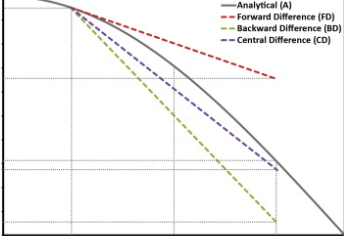
\includegraphics[width=0.45\textwidth]{figures/forward_vs_central_differentiation.png}
%       \caption{Comparison of Forward, Backward, \& Central Differentiation}
%       \label{forward_vs_central}
%       \end{center}
%       \end{figure}
%       \FloatBarrier
% 
% 
% 
% \paragraph{Method Specific Parameters:}
% 
% This section is specific to the method being used. In the above example it is specific to the $OPT++$ library. An additional example has been given below however if curious the reader is advised to see the default optimization methods located in:
% 
% \bigskip
% 
% \begin{lstlisting}
% $./data/cathode/optimization/optimization_methods_cathode/
% \end{lstlisting}
% or 
% \begin{lstlisting}
% $./data/mea/optimisation/optimization_methods_mea/
% \end{lstlisting}
% 
% \bigskip
% 
% In the following short example we are using a method from the SCOLIB library, the \texttt{coliny\_pattern\_search} algorithm. In this case we would change the \texttt{Optimization method = coliny\_pattern\_search} as appose to \texttt{optpp\_q\_newton} (\textit{line 17}).
% 
% We then would then replace (\textit{line 33 - 41}) in the above \texttt{opt\_app\_optimization} file  with the new method specific section.
% 
% \begin{lstlisting}
%      ######### Method Specific Parameters #########
%      #########	      SCOLIB (COLINY) 	   #########
%      #########----------------------------#########
% 	subsection coliny_pattern_search
% 	    set Initial Delta = 2		          # (default) 1
% 	    set Threshold Delta = 0.0001			# (default) 0.0001
% 	end
% \end{lstlisting}
% 
% 
% 
% \paragraph{Design Variables Section:}
% 
% The \texttt{Design Variables} Section is similar to the \texttt{opt\_app\_parametric} file except for two additional subsections.
% 
% \begin{enumerate}
%  \item 
% Scales
% 
% \item
% Step size
% \end{enumerate}
% 
% 
% \paragraph{Scales:} 
% 
% The scales section has two specifications 
% 
% \begin{enumerate}
%  \item 
% \texttt{scale\_method}
% 
% The \texttt{scale\_method} specifies whether you are going to specify no scale (\texttt{none}), \texttt{auto} scaling, \texttt{log}, or a \texttt{value}. In general it is good practice to specify a scale \texttt{value} as it allows the user to have a definite reference point, when using \texttt{auto} if there is a change in magnitude it will go unnoticed by the user in the final output solution. 
% 
% \item
% \texttt{scale} value
% 
% The scale value is the magnitude of the variable. For example if the variable is temperature we know that the scale is 100 as temperature is given in Kelvin (353 - 368 [K]). If its Nafion loading the scale is 0.1 as Nafion loading is a percentage (20 - 50 \%).
% \end{enumerate}
% 
% 
% 
% \paragraph{Step Size:}
% 
% The step size refers to the  $\bigtriangleup x $ in equations \ref{eq:Forward} \& \ref{eq:Central}. Greater the step size the less computations that will be required, however this also means the greatest error as the error is proportional to $(\bigtriangleup x)^2$. Therefore there is a fine trade off between computational time and error.
% 
% 
% 
% \paragraph{Responses Section:}
% 
% The Responses section has changes slightly compared to the \texttt{opt\_app\_parametric} file as we are now considering constrained optimization. If the above example was unconstrained optimization there would be no difference between the \texttt{opt\_app\_parametric} and \texttt{opt\_app\_optimization} responses section.
% 
% There are two types of constraints:
% 
% \begin{enumerate}
%  \item 
% Linear (Equality) Constraints (\textit{line 83})
% 
% \item
% Non-Linear Constraints (\textit{line 84})
% \end{enumerate}
% 
% In the above case we have three non-linear constrains and one linear constraint. 
% 
% 
% 
% \paragraph{Non-Linear Constraints:} 
% 
% Like the \texttt{Design Variable} section each nonlinear constraint requires a upper and lower bound (\textit{line 97 - 108}). If no finite upper or lower bound is to be specified $1e^{30}$ or $1e^{-30}$ can be specified.
% 
% 
% \paragraph{Linear (Equality) Constraints:} Unlike Non-Linear Constraints, Equality constraints only require the response variable to equal a value (\textit{line 112}). 
% 
% 
% 
% 
% 
% %-----------------------------------------------------------------------------------------------------
% %---------------------				Running FCST
% %---------------------			Multi-Objective Optimization
% %-----------------------------------------------------------------------------------------------------
% \section{Multi-Objective Optimization using OpenFCST} \label{sec:multi_objective_optimization}
% 
% To achieve multi-objective optimization we must first change three parameters.
% 
% \begin{enumerate}
%  \item 
% \texttt{Optimization strategy} (\textit{line 16})
% 
% \item
% \texttt{num\_design\_variables} (\textit{line 84})
% 
% \item
% \texttt{num\_objectives} (\textit{line 82})
% 
% \end{enumerate}
% 
% 
% 
% \paragraph{Optimization strategy}
% 
% When carrying out multi-objective optimization we can no longer optimize for just one objective function this is especially the case when an improvement of one objective comes at the expense of another (\textit{Performance \& Cost}). In order account for the additional objective function we incorporate weighting factors which specifies the importance of one objective over the other. The weights are referred to a \textbf{Pareto Weights} or \textbf{Pareto Set}.
% 
% In OpenFCST the default Pareto set is for two design variables. Figure \ref{pareto_set} below shows the  multi-objective weights for two design variables.
% 
% 
% 
% \FloatBarrier
% \begin{figure}[htbp]
% \begin{center}
% 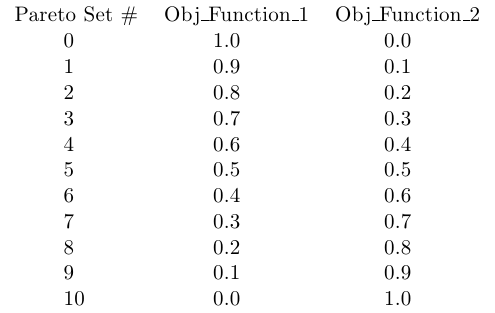
\includegraphics[width=0.4\textwidth]{figures/pareto_set.png}
% \caption{Pareto Set for 2 Design Variables}
% \label{pareto_set}
% \end{center}
% \end{figure}
% \FloatBarrier
% 
% 
% % \begin{center}
% %  
% % 
% % \begin{tabular}{lll}
% % Pareto Set \#	&Obj\_Function\_1 & Obj\_Function\_2 \\
% % 0	&	 1.0 	&	 0.0 	\\
% % 1	&	 0.9 	&	 0.1 	\\
% % 2	&	 0.8 	&	 0.2 	\\
% % 3	&	 0.7 	&	 0.3 	\\
% % 4	&	 0.6 	&	 0.4	\\
% % 5	&	 0.5 	&	 0.5 	\\
% % 6	&	 0.4 	&	 0.6 	\\
% % 7	&	 0.3 	&	 0.7 	\\
% % 8	&	 0.2 	&	 0.8 	\\
% % 9	&	 0.1 	&	 0.9 	\\
% % 10	&	 0.0 	&	 1.0 	\\
% % \end{tabular} 
% % 
% % \end{center}
% 
% 
% 
% \paragraph{num\_design\_variables \& num\_objectives:}
% 
% Once the \texttt{Optimization strategy} has been set to \texttt{pareto\_set} we then change both the num\_design\_variables \& num\_objectives to 2 or whatever number of design variables are specified.
% At present OpenFCST like most multi-objective engineering problems, considers only two design variables however this can be easily modified by changing the default Pareto set found in \texttt{dakota\_application.cc}. 
% 
% \section{DAKOTA Methods} \label{dakota_methods}
% 
% The following list is all of the current DAKOTA Methods available as of \textbf{1-MAY-2013}. The methods are known to work with OpenFCST and can be utilized. For detailed discriptions on the individual methods see DAKOTA manuals.
% 
% \begin{multicols}{3}
% \begin{enumerate}
%     \item 	\textbf{asynch\_pattern\_search}
%     \item       bayes\_calibration
%     \item       centered\_parameter\_study
%     \item       \textbf{coliny\_cobyla}
%     \item       \textbf{coliny\_direct}
%     \item       \textbf{coliny\_ea}
%     \item       \textbf{coliny\_pattern\_search}
%     \item       \textbf{coliny\_solis\_wets}
%     \item       \textbf{conmin\_frcg}
%     \item       \textbf{conmin\_mfd}
%     \item       dace
%     \item       dl\_solver
%     \item       dot
%     \item       dot\_bfgs
%     \item       dot\_frcg
%     \item       dot\_mmfd
%     \item       dot\_slp
%     \item       dot\_sqp
%     \item       \textbf{efficient\_global}
%     \item       fsu\_cvt
%     \item       fsu\_quasi\_mc
%     \item       global\_evidence
%     \item       global\_interval\_est
%     \item       global\_reliability
%     \item       importance\_sampling
%     \item       list\_parameter\_study
%     \item       local\_evidence
%     \item       local\_interval\_est
%     \item       local\_reliability
%     \item       \textbf{moga}
%     \item       \textbf{multidim\_parameter\_study}
%     \item       \textbf{ncsu\_direct}
%     \item       \textbf{nl2sol}
%     \item       nlpql\_sqp
%     \item       nlssol\_sqp
%     \item       nonlinear\_cg
%     \item       npsol\_sqp
%     \item       optpp\_cg
%     \item       \textbf{optpp\_fd\_newton}
%     \item       \textbf{optpp\_g\_newton}
%     \item       optpp\_newton			% Needs the Hessian Matrix
%     \item       \textbf{optpp\_pds}
%     \item       \textbf{optpp\_q\_newton}
%     \item       polynomial\_chaos
%     \item       \textbf{psuade\_moat}
%     \item       richardson\_extrap
%     \item       sampling
%     \item       \textbf{soga}
%     \item       stanford
%     \item       stoch\_collocation
%     \item       surrogate\_based\_global
%     \item       surrogate\_based\_local
%     \item       vector\_parameter\_study
% \end{enumerate}
% \end{multicols}
% 
% 
% 
% 
% 
% 
% 
% %-----------------------------------------------------------------------------------------------------
% %---------------------			Running OpenFCST
% %---------------------			Optimization Path-line
% %-----------------------------------------------------------------------------------------------------
% \section{Fuel Cell Design \& Optimization Using OpenFCST}
% As we've seen above OpenFCST also has the capabilities to perform optimization studies. Any application that is inherited from \texttt{OptimizationBlockMatrixApplication} has the appropriate interface to be used for optimization studies. Information on how to run optimization can be found in sections \ref{Optimization_using_FCST} \& \ref{sec:multi_objective_optimization}.
% 
% To perform optimization studies, OpenFCST interfaces with the open source libraries DAKOTA developed by Sandia National Laboratory. For more information about the DAKOTA library please \href{http://dakota.sandia.gov/software.html}{click here}. The OpenFCST developers have developed an interface so that DAKOTA and OpenFCST can interact seamlessly. 
% 
% \subsection{OpenFCST classes that interact with DAKOTA (Developers Only)}
% Interaction between OpenFCST and DAKOTA is achieved by using \texttt{simulation\_builder} which will call the \texttt{run\_optimization()} function.
% 
% When OpenFCST is run as seen in figure \ref{analysis_schematic} the OpenFCST code is called on once in order to run a specific data point. However in parametric or optimization studies we require multiple points to be evaluated. This requires the use of the DAKOTA libraries in order to change the variables after each iteration. The two main files used to interface with DAKOTA are:
% 
% 
% \begin{enumerate}
%  \item 
% \texttt{dakota\_direct\_interface}
% 
% \item
% \texttt{dakota\_application}
% 
% \end{enumerate}
% 
% Once the initial stages of the code have been carried out by \texttt{simulator\_builder}, \texttt{simulator\_selector}, and \texttt{dakota\_application}, declaring and initialing all the variables from the \texttt{main\_app\_}, \texttt{data\_app\_}, \& \texttt{opt\_app\_} files. The \texttt{main.cc} file then proceeds to the \texttt{run()} function in \texttt{simulator\_builder.cc} (see below) in order to run the simulation.
% 
% In the \texttt{run()} function we can see in line 10 where the code checks to see if its running an analysis or parametric/optimization study, as explained in \ref{main_application_file}. During parametric/optimization studies the code will enter line 12 and proceed to the \texttt{run\_optimization()} function in \texttt{simulator\_builder.cc}. 
% 
% 
% \begin{lstlisting}
% template<int dim>
% void SimulatorBuilder<dim>::run()
% {
% 	timer.restart();
%     
% 	if (run_tests) run_test();
% 	else
% 	{
% 		if (dakota_use || dakota_direct)
% 		{
% 			run_optimization();
% 		}
% 		else
% 		{
% 			//-- Select the application you want to run:
% 			app_lin = sim_selector->select_application();
% 			//-- Select the solver you want to run:
% 			newton = sim_selector->select_solver(app_lin.get());
% 			//-- Select the solving method you want to run, e.g. adaptive refinement:
% 			solver = sim_selector->select_solver_method(app_lin.get(), newton.get());
% 			// Here we have collected all information:
% 			deallog << "Run program using input file: " << simulator_parameter_file_name << std::endl;
% 			deallog.pop();
% 			solver->solve(simulator_parameter_file_name, param);
% 			timer.stop();
% 		}
% 	}
% 
% 	timer.stop();
% 	deallog.push("MAIN");
% 	deallog << "The program was executed in: " << timer.wall_time() << " seconds " << std::endl;
% 	deallog << "=============== END ====================" << std::endl;
% 	deallog.pop();
% 	
% }
% \end{lstlisting}
% 
% \bigskip
% 
% The main points to note once we enter the \texttt{run\_optimization()} function are:
% 
% \begin{enumerate}
% \item 
% Is DAKOTA running in Parallel or Series? (\textit{line 8})
% 
% As of \textbf{1-MAY-2013} Series is the only option available. This may change in the future.
% 
% \item
% Are we running a Non-Linear Least Squares (NLS) method or standard parametric/optimization routine? (\textit{line 16-25})
% 
% \end{enumerate}
% 
% \paragraph{Note:} 
% 
% These are questions that are answered in the \texttt{opt\_app\_} file explained earlier in section \ref{Optimization_using_FCST}.
% 
% 
% \bigskip
% 
% Once these have been specified the code will execute the \texttt{run()} function (\textit{line 28}), which begins the iterative loop until the parametric study has been complete or the stopping criteria have been met in optimization.An illistration of this can be see in figure \ref{dakota_optimization_interface} taken from Peter Dobson's 2012 paper.
% 
% 
% \begin{lstlisting}
% void SimulatorBuilder<dim>::run_optimization()
% {
% 	deallog.pop();
% 	if (dakota_direct)
% 	{
% 		// NOTE: Must declare these in order for parameter handler to not complain when reading the parameter file specified.
% 		//        Not exclusively required for dakota application to run.
% 		Dakota::ParallelLibrary parallel_lib;
% 		shared_ptr<Dakota::ProblemDescDB> problem_db(new Dakota::ProblemDescDB (parallel_lib));
% 		SIM::DakotaApplication optimization(problem_db, optimization_parameter_file_name);
% 		optimization.declare_parameters(param);
% 		optimization.manage_inputs(param);
% 
% 		Dakota::DirectApplicInterface* optimization_interface;
% 		
% 		if (optimization.use_NLS())
% 		{
% 			deallog<<"Entering DakotaLeastSquaresInterface"<<std::endl;
% 			optimization_interface = new SIM::DakotaLeastSquaresInterface<dim> (optimization, problem_db, param, sim_selector, simulator_parameter_file_name);
% 		}
% 		else
% 		{
% 			deallog<<"Entering DakotaDirectInterface"<<std::endl;
% 			optimization_interface = new SIM::DakotaDirectInterface<dim > (optimization, problem_db, param, sim_selector, simulator_parameter_file_name);
% 		}
% 		
% 		optimization.assign_interface(optimization_interface);
% 		optimization.run();
% 		
% 		deallog << "Optimization completed" << std::endl;
% .
% .
% .
% \end{lstlisting}
% 
% 
% If running a standard parametric/optimization routine, the following \texttt{dakota\_direct\_interface} function will be used.
% 
% \begin{lstlisting}
% template <int dim>
% int DakotaDirectInterface<dim>::derived_map_ac(const Dakota::String& ac_name)
% \end{lstlisting}
% 
% If running a Non-Linear Least Squares (NLS) method, the following \texttt{dakota\_direct\_interface} function will be used.
% 
% \begin{lstlisting}
% template <int dim>
% int DakotaLeastSquaresInterface<dim>::derived_map_ac(const Dakota::String& ac_name)
% \end{lstlisting}
% 
% 
% \FloatBarrier
% \begin{figure}[htbp]
% \begin{center}
% 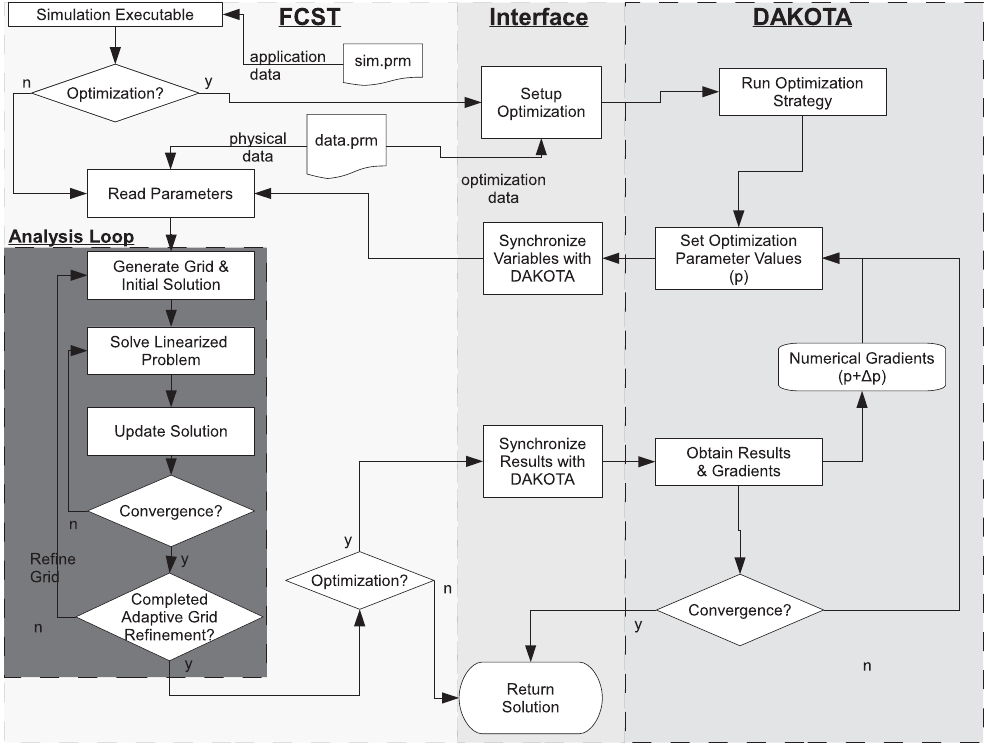
\includegraphics[width=1\textwidth]{figures/fcst_dakota_interface_Dobson.png}
% \caption{Schematic of Fuel Cell Analysis Code and DAKOTA Optimization Interface (Dobson, 2012)}
% \label{dakota_optimization_interface}
% \end{center}
% \end{figure}
% \FloatBarrier

%%===============================================================
%%===============================================================
%%===============================================================
%%===============================================================
\chapter{Post-processor}
%%===============================================================
%%===============================================================
%%===============================================================
% Authors: M. Secanell
%%===============================================================

OpenFCST can output results in many different formats using the deal.II output parser. OpenFCST developers however output the solution in .vtu format and use the open-source post-processing software \htmladdnormallink{Paraview}{http://www.paraview.org/} to analyze their results. ParaView is an open-source data analysis and visualization program. It can run on multiple operating systems.
ParaView users can quickly analyze their data visually using qualitative and quantitative methods already implemented in the software. 

A ParaView tutorial can be found at the following \htmladdnormallink{site}{http://www.youtube.com/watch?v=w-65jufR-bc}. Wolfgang Bangerth and Timo Heister recently published a very good lecture on how to use Paraview at the following \htmladdnormallink{site}{http://www.math.tamu.edu/~bangerth/videos.676.32.html}.

%%===============================================================
%%===============================================================
%%===============================================================

%%===============================================================
\part{Developer's Reference Guide (Under development)}
%%===============================================================
%%===============================================================
\chapter{Setting up the development environment for OpenFCST}
%%===============================================================
%%===============================================================
%% Author: Phil Wardlaw and Marc Secanell
%%===============================================================
%%===============================================================

In the following sections we describe how to create an OpenFCST branch where you can develop your own code and commit the changes to the OpenFCST team. Also, we show how to setup KDevelop, the program we recommend for compiling and modifying code in OpenFCST.

%%===============================================================
\section{Getting the \texttt{development} version of OpenFCST}

The development version of OpenFCST is hosted on a private repository on BitBucket. In order to access the \texttt{development} branch of OpenFCST, please contact the developers. You can also develop code from the GitHub version of the code and then submit your changes to the OpenFCST team. We will then merge the changes into the code for the next release.

If you want to modify OpenFCST, you will need to first clone the development version of OpenFCST, and then create your own branch of the code. Afterwards you can then modify, test, and commit this branch. Once your branch has been tested and validated, you can issue a Pull Request. Then, several senior OpenFCST developers will look at the code, suggest changes, and finally merge the code into the stable development version of OpenFCST. The stable development version of OpenFCST is then used to create new releases.

%%=======
\subsubsection{Creating a new branch}

Committing changes to the development branch is not allowed. You will need to create a pull request of your branch. Every user can create their own branch of OpenFCST. The recommended convention for branch usage is that each user creates their own branch for each issue in OpenFCST they would like to address. The naming convention is: \texttt{username/issue\_name}. For example, if Secanell wants to create an issue to fix a bug on postprocessing, the branch would be named \texttt{secanell/postprocessing}.
 
To create a branch, users can either create it on their own machine and then push it to BitBucket or create the branch directly on BitBucket. If the branch is created on BitBucket, then, in order to checkout the branch to the appropriate machine, the user needs to issue the following command:
\begin{lstlisting}
  git branch branch_name origin/branch_name  
  git checkout branch_name
\end{lstlisting}  
Both steps can be performed simultaneously with
\begin{lstlisting}
git checkout -b username/issue\_name origin/username/issue\_name}
\end{lstlisting}  
 
If the branch is created on the local repository first using \texttt{git checkout -b branch\_name}, then you can commit it to BitBucket, i.e. remote server, using \texttt{git push -u origin branch\_name}.
The \texttt{-u} flag means that from now on your branch \texttt{branch\_name} will track the branch on BitBucket.

%%=======
\subsubsection{Adding, changing, staging, committing and pushing}
 
Once the branch is created, users can work on that branch for as long as needed. Users can make changes and commit the changes to their local repository using:
\begin{lstlisting}
  git add file_name
  git commit -m "message about commit"
\end{lstlisting} 
Please DO NOT use \texttt{git add *} or \texttt{git add -u} as you then have little control over what you are staging to be  committed. Using \texttt{git status} you can see which files have changed so that you can add them
as appropriate.
 
To commit to BitBucket, you can use:
\begin{lstlisting}
  git push origin branch_name
\end{lstlisting} 

%%=======
\subsubsection{Request for branch to be merged into development}

Once you have finished fixing the issue you created the branch for, you need to follow these three steps:
\begin{enumerate}
 \item Update your origin information using: \texttt{git remote update} (this will update all your local information regarding the branches on BitBucket).
 \item Merge your branch with the latest version of development using: \texttt{git merge origin/development}. This is VERY important. The administration will not accept any pull requests that 
   have not been fast-forwarded to the \texttt{origin/development branch}.
 \item Issue a pull request in BitBucket
\end{enumerate}

 
There are three main branches  
\begin{itemize}
 \item Master branch: Stable version of OpenFCST (no pull requests will be accepted to this branch).
 \item Development branch: The most up-to-date version of OpenFCST, personal branches should be started from this branch and all pull requests should be submitted to this branch.
 \item Release branch: Branch containing the latest release of OpenFCST.
\end{itemize}

%==================
\subsubsection{Workflow for new development}

If you want to develop new code, please follow these steps: 
\begin{itemize}
 \item Clone the repository using:\\
  \texttt{git clone https://your\_username@bitbucket.org/ESDLab/openfcst.git}
 \item Create a new branch related to the new component/issue you would like to work on using: \texttt{git checkout -b name\_branch}. Note: The command above will create a branch named \texttt{name\_branch} and will checkout that branch so you are ready to work.
 \item Once you are done with the development, ask for a pull request to merge your branch to the development branch.
\end{itemize}
Note: Merges to Master will be rejected without review.

A reminder: when developing code, please work on Debug mode (the current version gives an error once the program finishes in debug mode, please ignore for now as we will be working on fixing this) and test on Debug and Release mode before issuing a pull request. We are aware that running tests in Debug is more time consuming, but the issues that we have in debug mode have occurred precisely because we did not test on that mode.


%%===============================================================
\section{Setting up OpenFCST under KDevelop} \label{setting_up_fcst}
%%===============================================================

If you are going to be developing new routines for OpenFCST, we recommend that you use either KDevelop or Eclipse to modify, compile, and debug new code. In order to setup a KDevelop project with OpenFCST, follow the steps below:
\begin{itemize}
 \item Compile OpenFCST using the provided script, i.e. \texttt{openFCST\_install}. This will configure all the folders you will be using during configuration  of KDevelop. This step is not required, however, it is recommended and the steps below assume OpenFCST has been installed and that the Build and Install directories already exist on your computer.
 \item Go to Project $>$ Open/Import Project... Go to the OpenFCST folder, enter the \texttt{src} folder and then, select the \texttt{CMakeLists.txt} file in \texttt{openfcst/src} (see Figure \ref{fig:setup_KDevelop}). In the next window, enter the name of the project, e.g. OpenFCST, and select \texttt{CMake Project Manager}. At this point, the project should either appear or prompt another window asking for the Build folder. If the latter is the case, point KDevelop to the Build folder in the main folder of OpenFCST. Then, the project import is complete and the project menu will appear on the left hand side.
 \item If you want to modify the compilation parameters in the project, you can do that by right clicking on the project name and selecting \texttt{Open Configuration...}. The menu in Figure \ref{fig:setup_KDevelop_options} would appear. You should not need to modify many parameters, however several parameters are handy. The variable OPEN\_FCST\_BUILD\_TYPE allows you to compile the code in Debug or Release mode. The former is used during code development as it provides a lot more information about errors, the latter is best for simulations as the code can be several times faster. Another useful parameter is OPEN\_FCST\_DIMENSIONS. If set to 2, it will only compile a 2D version of OpenFCST. If you compile with 3, it will compile a 3D version. If you compile with 1, it will compile both 2D and 3D versions. Finally, on the left menu if you click on Make, the parameter \texttt{Number of simultaneous jobs} sets up the compilation for using as many threads as specified. 
\end{itemize}

\begin{figure}[btp]
\begin{center} 
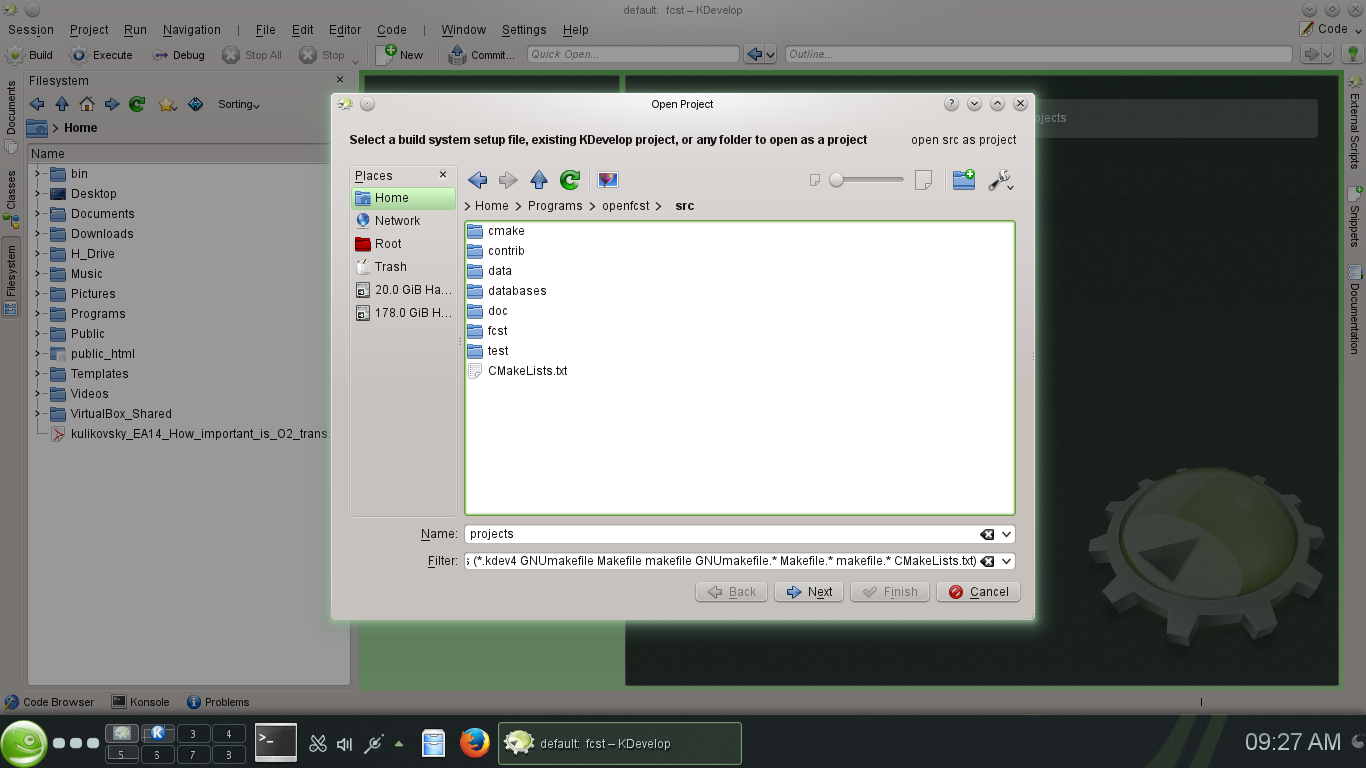
\includegraphics[width=\textwidth]{./figures/kdevelop_1.png}
\caption{Initial window in KDevelop to import a CMake project.}
\label{fig:setup_KDevelop}
\end{center}
\end{figure}

\begin{figure}[btp]
\begin{center} 
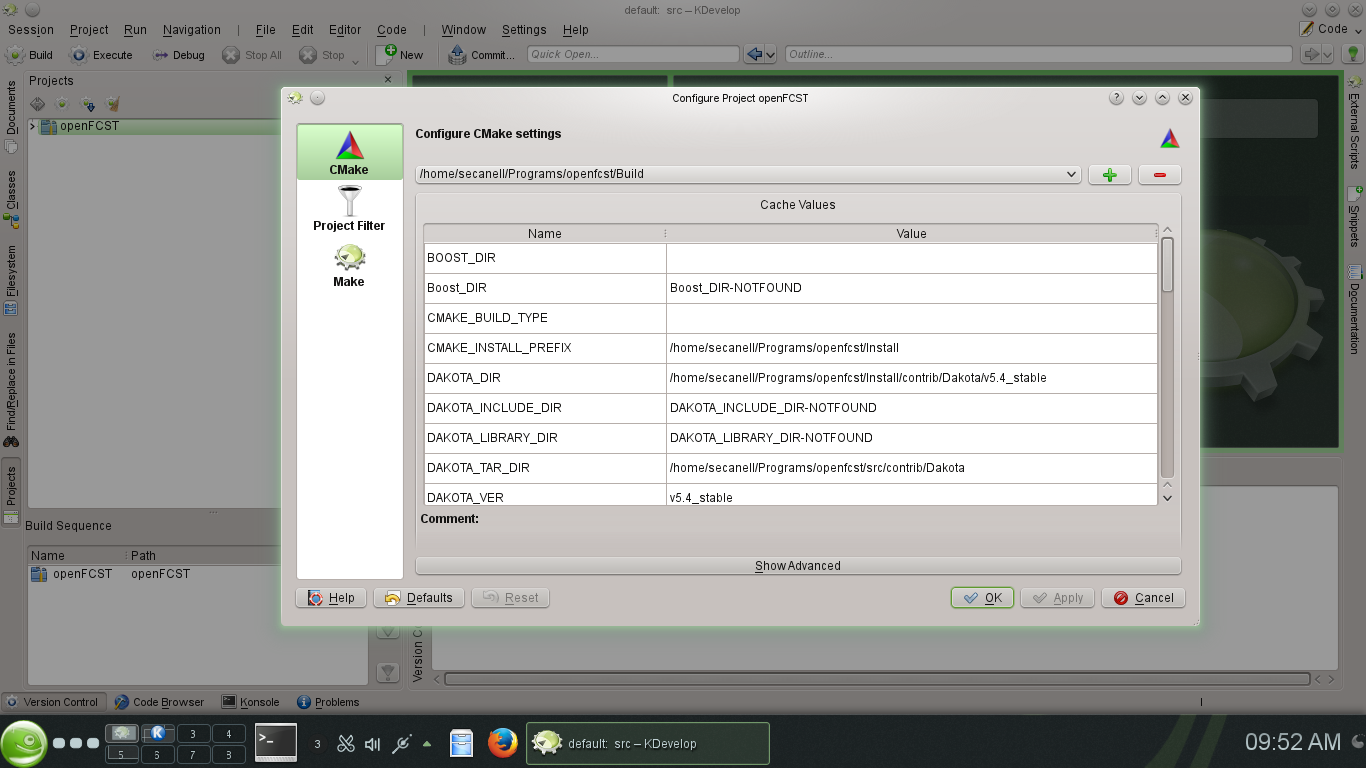
\includegraphics[width=\textwidth]{./figures/kdevelop_2.png}
\caption{Configuring your CMake project in KDevelop.}
\label{fig:setup_KDevelop_options}
\end{center}
\end{figure}

Next, we will setup the environment to run and debug OpenFCST within KDevelop by following the steps below:
\begin{itemize}
 \item Go to \texttt{Run $>$ Configure Launches... }. The window in Figure \ref{fig:example_KDevelop} will open.
 \item Select either Global or your project option (we recommend your project).
 \item Press the '+' button on the top of the window. Once you press this botton, a new option will open under either Global or OpenFCST. 
 \item Select \texttt{New Native Application Configuration}, then on the right of the window, under Executables, enter the OpenFCST binary file, i.e. \texttt{OpenFCST\_directory/Install/bin/fuel\_cell-2d.bin}. Under Behaviour, in Working Directory enter the data folder from which you would like to run the code. In Arguments, enter the main parameter file, see Figure \ref{fig:example_KDevelop}.
 \item Your code is set! Click OK on the window. Now, you can run the code with the \texttt{Execute} and \texttt{Debug...} buttons on the menu. If you have more than one \texttt{New Native Application Configuration} configured, rename them by clicking on the same. Then, you can switch between application configurations using \texttt{Run $>$ Current Launch Configuration}
\end{itemize}
 
\begin{figure}[btp]
\begin{center} 
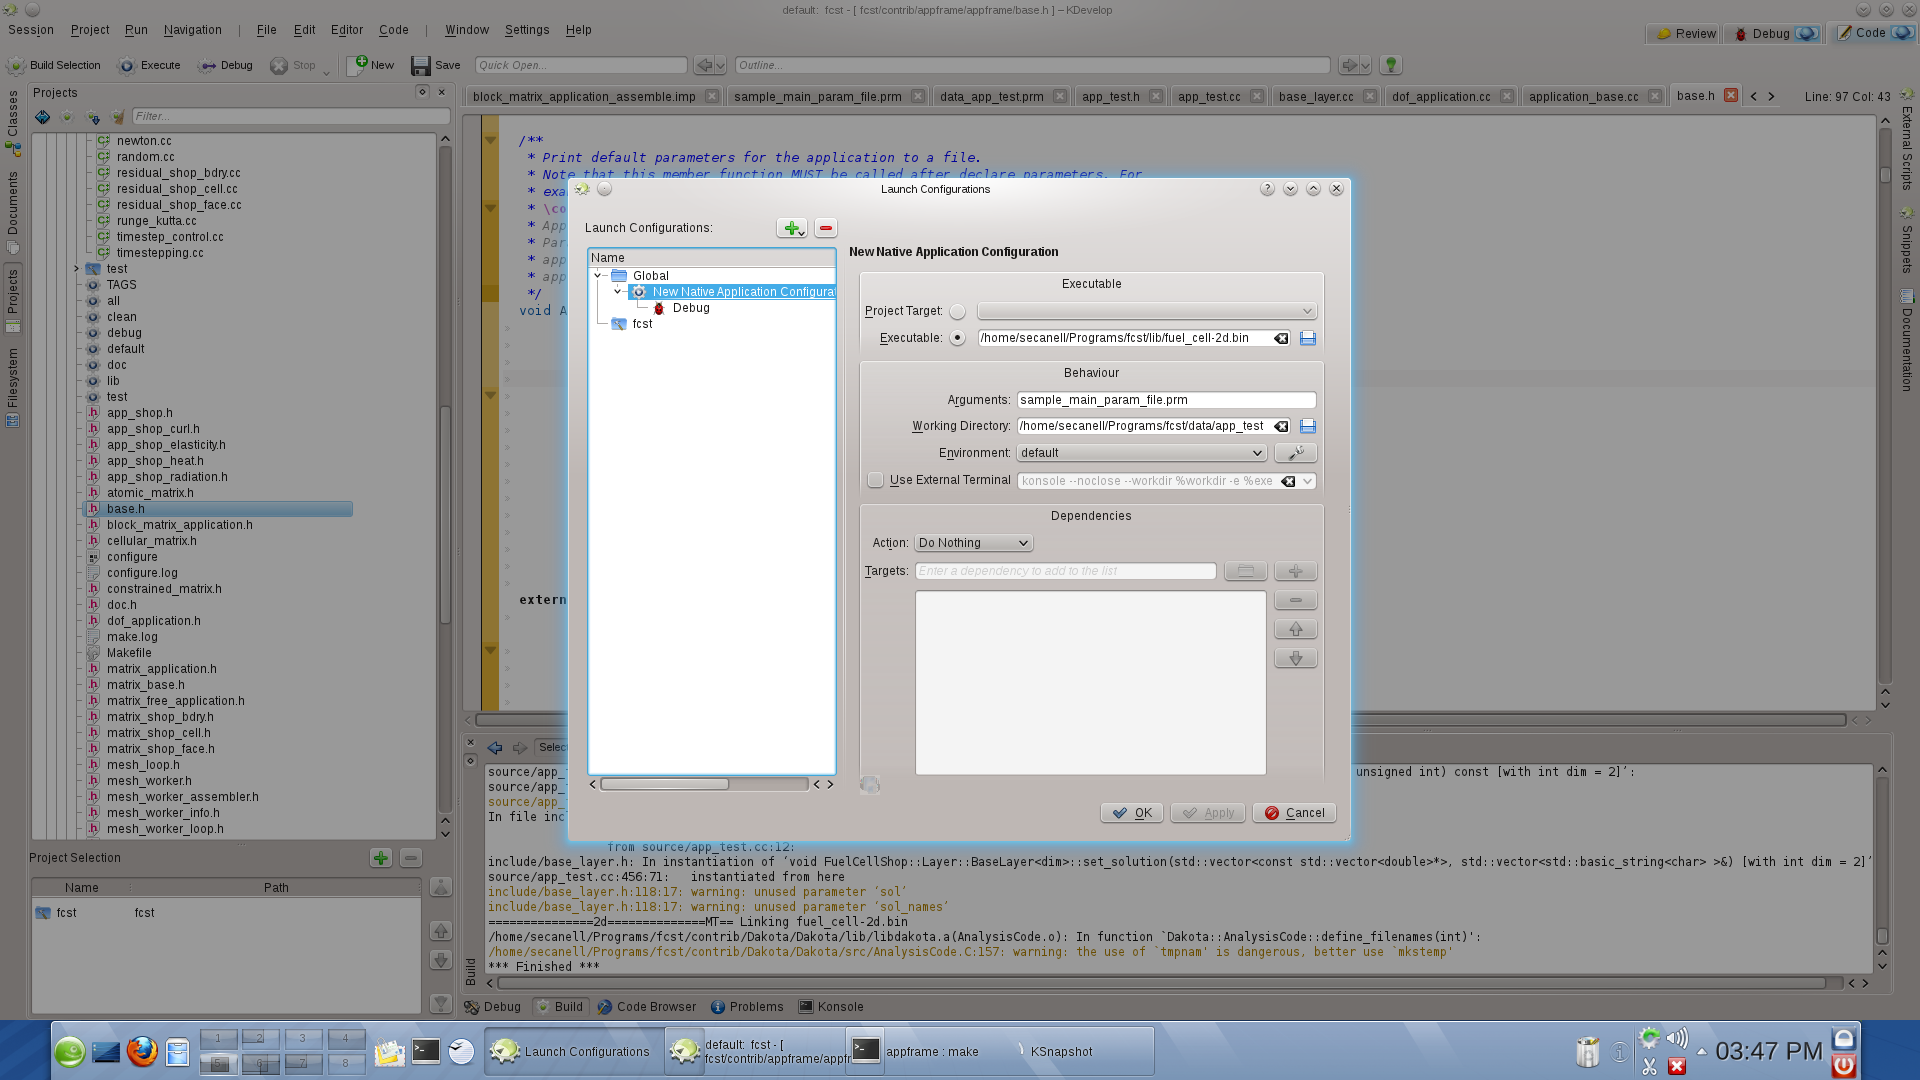
\includegraphics[width=\textwidth]{./figures/LaunchConfigurations.png}
\caption{Configuring Launches in KDevelop.}
\label{fig:example_KDevelop}
\end{center}
\end{figure}

\subsection{Formatting OpenFCST files}

All files should start with the following information:

\begin{lstlisting}
// ----------------------------------------------------------------------------
//
// FCST: Fuel Cell Simulation Toolbox
//
// Copyright (C) 2009-20XX by Energy Systems Design Laboratory, University of Alberta
//
// This software is distributed under the MIT License
// For more information, see the README file in /doc/LICENSE
//
// - Class: class_name
// - Description: short description of class
// - Developers: name_developers, affiliation
// - Id: $Id$
//
// ----------------------------------------------------------------------------
\end{lstlisting}
 
In order to keep the formatting of all files consistent, it is recommended to use the space style for code readability. In KDevelop, set your formatting options:
\begin{itemize}
\item In the main menu, go to Setting $>$ Configure Editor.
\item In the 'Editing' section, select the Indentation tab.
\item Set 'Indent Using' to \textit{Spaces}, and set the spacing to \textbf{4 characters}. 
\end{itemize}
%%===============================================================
%%==============================================================
%Needs to be re-written: %%===============================================================
%%===============================================================
\chapter{OpenFCST \texttt{src} structure}
%%===============================================================
%%===============================================================

This chapter discusses the sections of the source folder in OpenFCST, i.e., the \texttt{src} folder.
%%===============================================================
\section{Directory tree}
%%===============================================================
OpenFCST contains six subfolders, namely:
\begin{itemize}
 \item \texttt{fcst} is the most important folder in OpenFCST \texttt{src}. It contains the include (*.h) and implementation (*.cc) files for OpenFCST. Inside this folder the following sub-folders can be found:
 \begin{itemize}
  \item \texttt{include} contains all include files (*.h)
  \item \texttt{source} contains all source files (*.cc)
  \item \texttt{GUI} contains all include (*.h) and implementation (*.cc) files for the OpenFCST graphical user interface.
  \item \texttt{unit_tests} contains all the unit tests for OpenFCST. Unit tests are used to check for the functionality of different classes in OpenFCST. All this tests are run in our test suite in order to make sure that OpenFCST continues to run as expected as we are more functionality.
  \item \texttt{cmake} contains the compilation configuration files for CMake.
 \end{itemize}
 \item \texttt{doc} contains all documentation. This includes a main HTML file to access all documentation (the \texttt{index.html} in the \texttt{doc} folder), this User’s Manual in HTML (in the \texttt{RefGuide} folder), and the class documentation in HTML (in \texttt{html} folder).
 \item \texttt{examples} contains a set of input parameters and examples to learn how to use OpenFCST. This examples are also used in our nightly test environment using CDash. Therefore, this folder should not be modified. All subfolders \texttt{regression} contain a script to run the tests and a reference solution.
 \item \texttt{test} is used for our nightlyt tests in CDash (see section \ref{sec:CTest}) and also for testing the code using the script \texttt{run\_tests}.
 \item \texttt{my_data} is a dummy folder created so that users can store their data there.
 \item \texttt{contrib} contains the contributing libraries to OpenFCST. These are open source libraries that have been developed by other people and are used within OpenFCST. This include AppFrame (developed by G. Kanschat) and DAKOTA (developed by Sandia National Labs). Note that the codes have been modified.
 \item \texttt{cmake} contains the compilation configuration files for CMake.
\end{itemize}

The main program file is main.cc in FuelCell/source. This file creates:
\begin{itemize}
 \item A NewtonExecution object. This object is used to implement the mesh adaptive loop
 \item NewtonExecution object. This object is used to implement the mesh adaptive loop
 \item A linear application that implements the fuel cell equations (linearized version of them). There are several linear applications. The linear solver implements:
	\begin{itemize}
 	\item $cell\_residual()$: This member function is called by $dof\_application.c$c in AppFrame in order to
implement the residual. $cell_residual()$ is in charge to compute the residual for a given cell.
 	\item $cell\_matrix()$: This member function is called by $block\_matrix\_application.cc$ (via
optimization\_block\_matrix\_application.cc) and is used to assemble the cell matrix. $block\_matrix\_application.cc$
uses this information to assemble the stiffness matrix for the complete problem.
 	\item solve(): This member function is used to solve the linear system.
	\end{itemize}
\end{itemize}

%%===============================================================
\section{Understanding OpenFCST Architecture}
%%===============================================================

\hl{EXPLAIN WHAT IS AN APPLICATION, PHYSICS, ETC.}

%%===============================================================
\section{Understanding OpenFCST Applications: The OpenFCST tutorials}
%%===============================================================

OpenFCST contains several tutorials to get you started developing your own applications. Currently two tutorial applications have been developed
\begin{itemize}
 \item Cathode application
 \item Cathode and membrane application
\end{itemize}

You can find these two tutorials in the Modules section of the DOxygen documentation, i.e. in file \texttt{/doc/html/modules.html}. All OpenFCST developers learnt to develop applications by first reading these tutorials. If you are developing new physics classes, then you will be relying heavily on classes from the \htmladdnormallink{deal.II}{http://www.dealii.org/} finite element libraries. If this is the case, the OpenFCST developers would recommend any new developers to look at the tutorials provided in the \htmladdnormallink{deal.II}{http://www.dealii.org/} website.

\hl{!!!!!!!!!!!!!!! IS THERE ANYWAY WE CAN INSERT THE TUTORIALS FROM DOXYGEN HERE !!!!!!!!!!!!!!!}

%%===============================================================
\section{OpenFCST Applications}
%%===============================================================

\subsection{Data files}

It is recommended that every application also contains a data file in \texttt{/fcst/trunk/data} with a folder name corresponding to the name of the application. The data folder should contain four sub-folders as follows
\begin{itemize}
 \item analysis: This folder contains default (and well documented) main, data and mesh input files to run a sample analysis problem.
 \item parametric: This folder contains default (and well documented) main, data, mesh and optimization files to run a parametric study using OpenFCST and Dakota
 \item optimization: This folder contains default (and well documented) main, data, mesh and optimization files to run a parametric study using OpenFCST and Dakota
 %\item testing: This file contains the main, data and mesh input files used to test that the application is returning expected results during the CDash nightly tests. The file also contains a file named \texttt{test_results.dat} with the expected solution.
\end{itemize}



%%===============================================================
\section{Namespace structure}
%%===============================================================

OpenFCST contains four namespaces, namely
\begin{itemize}
 \item \textit{FuelCell}
 \item \textit{FuelCellShop}
 \item \textit{AppFrame}
 \item \textit{AppFrameShop}
\end{itemize}

Namespaces \textit{AppFrame} and \textit{AppFrameShop} designate member function in the contributing library \textit{AppFrame} which was originally developed by Dr. Guido Kanschat at the University of Heidelberg and is currently maintained by Dr. Guido Kanschat and the authors of Fuel Cell Simulation Toolbox (OpenFCST).

Namespaces \textit{FuelCell} and \textit{FuelCellShop} form the core of OpenFCST. Namespace \textit{FuelCell} contains an Application and InitialSolution namespace as well as several classes such as OperatingConditions. Application namespace contains classes that can be used to solve a specific problem such as fluid flow in a channel, or the phyiscal processes occuring in the cathode of a fuel cell. Based on the nature of the application, two types of classes are available:
\begin{itemize}
 \item \textit{AppFrame::DoFApplication}
 \item \textit{AppFrame::ApplicationCopy}
\end{itemize}
Figure \ref{fig:AppBase_Tree} shows an overview of the two types of applications. 

\begin{figure}[btp]
\begin{center} 
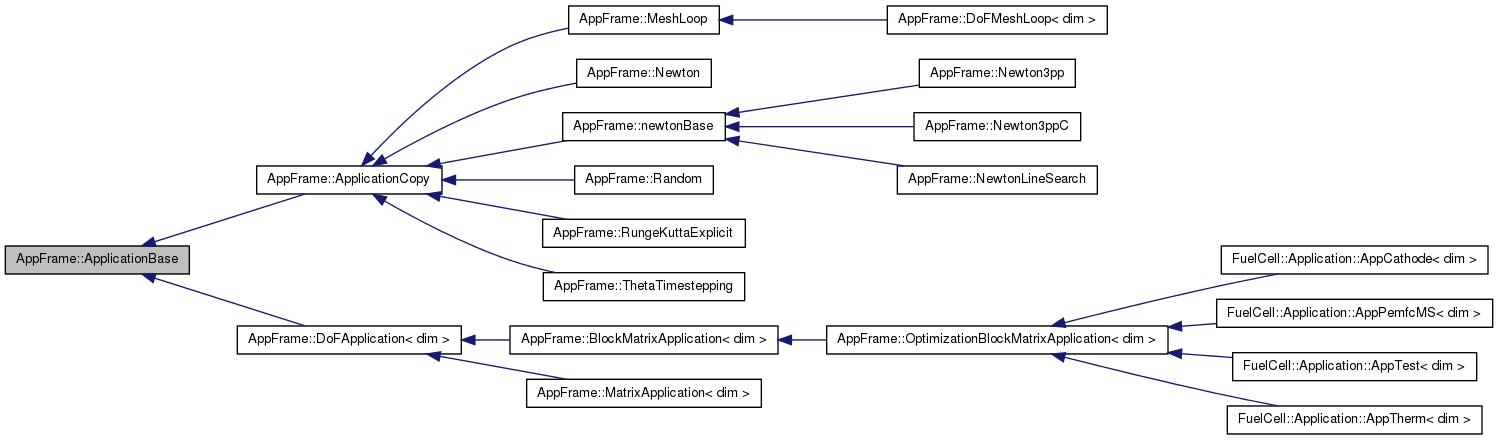
\includegraphics[width=\textwidth]{./figures/classAppFrame_ApplicationBase__inherit__graph.jpg}
\caption{Inheritance tree for ApplicationBase}
\label{fig:AppBase_Tree}
\end{center}
\end{figure}

Classes inherited from \textit{AppFrame::DoFApplication} are used when we need to implement the governing equations of the physical problem, i.e. the weak from of the partial differential equations. Class \textit{AppFrame::DoFApplication} implements all the methods used to assemble the right hand side, i.e. it contains a Triangularization (domain mesh), a deal.ii DoFHandler and several other objects to loop over cells. Class \textit{AppFrame:: BlockMatrixApplication} is a child of \textit{AppFrame::DoFApplication} and contains additional functionality in order to assemble and store the global system matrix into a BlockMatrix object. Finally, class \textit{AppFrame:: OptimizationBlockMatrixApplication} implements optimization functionality such as functional evaluation. OpenFCST applications that require assemble of a system matrix and right hand side are inherited from this application such as \textit{FuelCell::AppCathode}. 

Figure \ref{fig:AppCathode_Tree} provides an example of the inheritance tree for \textit{FuelCell::AppCathode}. AppCathode inherits all the functionality of of \textit{AppFrame::DoFApplication}, \textit{AppFrame::BlockMatrixApplication} and \textit{AppFrame:: OptimizationBlockMatrixApplication}. The responsibility of the OpenFCST applications in namespace \textit{FuelCell} is to initialize all the variables and to implement three main routines
\begin{itemize}
 \item cell\_matrix()
 \item cell\_residual()
 \item solve()
\end{itemize}
The first two routines are used to implement the element-wise system matrix and the element-wise right hand side. The latter member function is use to solve the global finite element problem. A tutorial on how to develop an application can be found in the HTML documentation.

Classes inherited from \textit{AppFrame::ApplicationCopy} are used to implement iterative loops. For example, when solving a nonlinear problem, a linear problem is solved iteratively. Therefore, classes that inherit from \textit{AppFrame::ApplicationCopy} usually contain an application that inherits from \textit{AppFrame::DoFApplication}. In terms of OpenFCST, OpenFCST developer will usually implement \textit{AppFrame::DoFApplication} and use the already implemented classes of type \textit{AppFrame::ApplicationCopy} in order to develop iterative loops for adaptive refinement, nonlinear problems and time-dependent problems.

As an example, in simulation\_builder.cc the following process is employed to solve a nonlinear problem:
\begin{lstlisting}
	//-- Select the application you want to run:
	app_lin = sim_selector->select_application();
	//-- Select the solver you want to run:
	newton = sim_selector->select_solver(app_lin.get());
	//-- Select the solving method you want to run, e.g. adaptive refinement:
	solver = sim_selector->select_solver_method(app_lin.get(), newton.get());
	// Here we have collected all information:
	deallog << "Run program using input file: " 
		<< simulator_parameter_file_name << std::endl;
	deallog.pop();
	solver->solve(simulator_parameter_file_name, param);
\end{lstlisting}
In the code above, first an OpenFCST application that inherits from \textit{AppFrame::DoFApplication} is created. Then, the application that is used to solve the linear system of governing equations at each iteration is handed in to a Newton solver that inherits from \textit{AppFrame::ApplicationCopy}. This solver is in turn handed to another solver that inherits from \textit{AppFrame::ApplicationCopy} and that implements an adaptive refinement loop.

Namespace \textit{FuelCell} is therefore a place holder for applications of type \textit{AppFrame::DoFApplication}. This applications are the core of OpenFCST since the assemble the system of equations that need to be solved. Users can develop their own applications by inheriting \textit{AppFrame::OptimizationBlockMatrixApplication} and re-implementing declare\_parameters(), initialize(), cell\_residual(), cell\_matrix() and solve() as shown in Figure \ref{fig:AppCathode_Tree} and explained in detail in the tutorial program for AppCathode. If the problem requires solving the problem iteratively such as in nonlinear and transient problems, the application will be handed over to an application of type \textit{AppFrame::ApplicationCopy} to be solved iteratively.

\begin{figure}[btp]
\begin{center} 
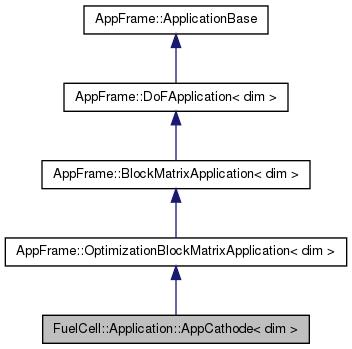
\includegraphics[scale=0.75]{./figures/classFuelCell_Application_AppCathode__inherit__graph.jpg}
\caption{Inheritance tree for FuelCell::Application::AppCathode}
\label{fig:AppCathode_Tree}
\end{center}
\end{figure}


The namespace \textit{FuelCellShop} is divided into several other namespaces as follows
\begin{enumerate}
 \item Material namespace: Specify the properties of common materials used in fuel cells. Examples of material classes include $PureGas$ baseclass.
 \item Layer namespace: Specify the different MEA components in a fuel cell. A BaseLayer has been developed in order to standarize this classes. They contain $material_id$ and $bondary_id$ elements to be able to relate the layer to the mesh as well as many other properties. Layer classes contain material classes in them that are used in order to obtain the appropriate physical parameters of the layer. Some layers are homogeneous and some are heterogeneous and anisotropic.
 \item Matrix namespace (OLD): Used to assemble the governing equations of a system. For linear problems this class implements the stiffness matrix for a givem equation. For nonlinear problems it generally includes $\frac{\partial R}{\partial \vec{u}}$. This matrix is used to calculate the step size in a Newton solver.
 \item Residual namespace (OLD): Used to assemble the governing equations of the system. For linear system these classes contain the right hand side of the problem. For nonlinear systems they contain the residual at the previous iteration, i.e. $R(\vec{u})$.
\end{enumerate}

%%===============================================================
\section{Layers Namespace}
%%===============================================================

A Layer in OpenFCST is used to define the properties of a cell in a finite element mesh. A Layer can be formed with with a single material or, in the case of composite layers such as a gas diffusion layer or a catalyst layer, it contains several materials and reaction parameters which are then used to compute the effective properties. An example of a catalyst layer is shown in Figure \ref{fig:catalystlayerexample}. 

\begin{figure}[tbp]
\begin{center}
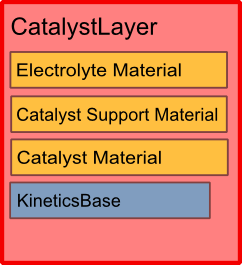
\includegraphics[width=0.25\textwidth]{figures/catalyst_layer_diagram.png}
\label{fig:catalystlayerexample}
\caption{Layer namespace structure}
\end{center}
\end{figure} 

The FuelCellShop::Layers namespace contains all the layers available with OpenFCST. All layers inherit from BaseLayer as shown in Figure \ref{fig:layerbase}. BaseLayer is a virutal class. An object of this class should never be created. BaseLayer simply provides common member functions and data members that apply to all layers. 



The layer classes contain a member function named set\_solution() which parses the uni

\begin{figure}
\begin{center}
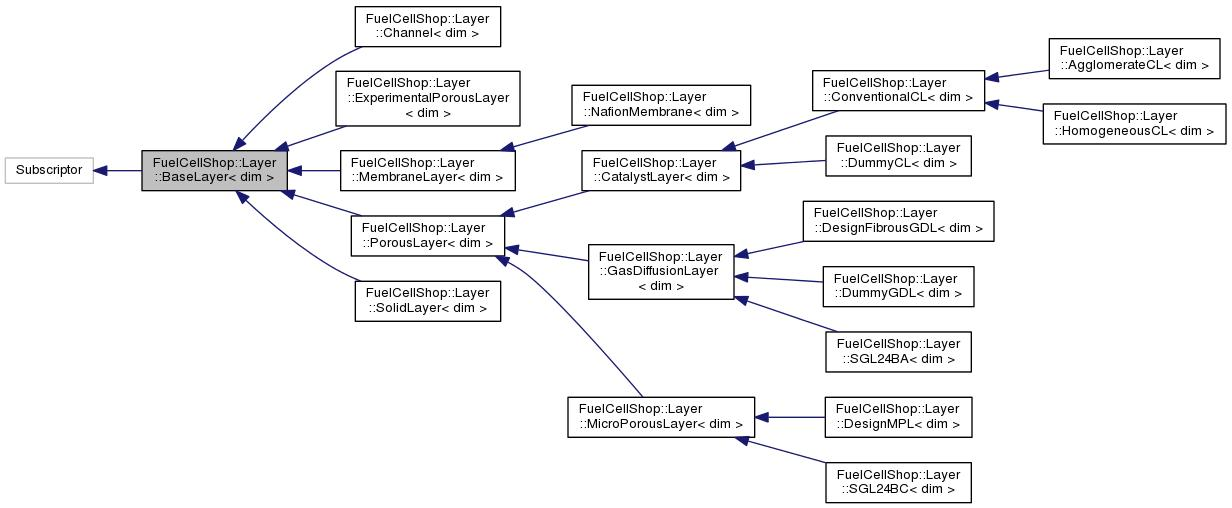
\includegraphics[width=0.9\textwidth]{figures/classFuelCellShop_1_1Layer_1_1BaseLayer__inherit__graph.jpg}
\label{fig:layerbase}
\caption{Layer namespace structure}
\end{center}
\end{figure} 





%%===============================================================
\section{Materials Namespace}
%%===============================================================

No materials contain a set solution. Materials will only set specific variables using a routine such as set\_temperature(double).






%%===============================================================
%%===============================================================
\section{Contributing libraries}

OpenFCST is distributed with copies of deal.II, Appframe, Dakota, COLDAE, ALGLIB and cpptest. These projects reside in the subdirectory \texttt{contrib/}. Please note that these projects are copyrighted by others than the OpenFCST authors and are covered by different licenses. For details, consult their respective webpages. A copy of their respective license is provided with the code. Inside each contributing library folder you will also find a file called \texttt{README.txt}. This file contains a list of any modifications that the OpenFCST developers have made to the contributing libraries. Note that some OpenFCST authors also contribute to the additional libraries. For example, Valentin Zingan is also contributor of the deal.II libraries.

\subsection{\texttt{APPFRAME}}
AppFrame was originally developed by Dr. Guido Kanschat at Texas A \& M and it is not continued to be developed by the ESDLab group. AppFrame is a framework to develop a chain of applications. The idea of these application classes is the possibility to build a chain out of these in order to have several predefined nested solvers. For this, we distinguish applications roughly in two classes, both derived from ApplicationBase:
\begin{itemize}
 \item Terminal applications, which implement the real finite element code like computing residuals on mesh cells, assembling matrices and solving linear systems.
 \item Non-terminal applications derived from ApplicationCopy; these usually implement a new solve() function as an iterative solver around another application. They implement all functions of the ApplicationBase interface, either forwarding them to the next inner application by ApplicationCopy or by providing their own implementation.
\end{itemize}

Usually a class in a chain communicates values with its next outer class through function arguments. Nevertheless, at least the terminal application will require values from even outer applications in the chain in order to compute residuals and matrices correctly. For these, the mechanism of named data provided by ApplicationData was introduced. Each class can store auxiliary data under a unique name there for use in inner iterations.

\subsubsection{Class DoFApplication}
This class it the parent of all terminal applications. It is the base class for applications requiring a Triangulation and a handler for degrees of freedom.

The mesh as well as the dof handler may be created by this class, which is the default, or they may be provided by another object, in which case they must be specified in the constructor.

Note that in this class the received or created dof handler is associated to the finite element given by the argument "Element" on the parameter file. Therefore, this class in not responsible to generate the system of equations to be solved, only to initialize the dof handler "Element" can either be a single element of a FESystem. In the latter case, the nomenclature used in the paramter file is: set Element = FESystem[element1\_type(element1\_degree)\textasciicircum number\_of\_elements1-...-elementN\_type(elementN\_degree)\textasciicircum number\_of\_elementsN] Example: set Element = FESystem[FE\_DGQ(0)-FE\_Q(1)\textasciicircum 2]

\subsubsection{Class BlockMatrixApplication}
\textbf{Text needed here}


\subsection{\texttt{COLDAE} Interface}
The class \texttt{DAESolver}, declared in \texttt{DAE\_solver.h} and defined in \texttt{DAE\_solver.cc}, provides an interface to the \texttt{Fortran 77} boundary-value differential algebraic equations (DAEs) code \texttt{COLDAE}.  The code solves DAEs the consists of a system of mixed-order ODEs
\begin{equation*}
  u_{i}^{(m_{i})} =  f_{i} ( x; z(u(x)), y(x) ), \quad    i = 1, ... ,c,
\end{equation*}
and algebraic constraints 
\begin{equation*}
  0   =  f_{i}( x; z(u(x)), y(x) ), \quad   i = c+1,...,c+d,
\end{equation*}
for $a < x < b$.   The DAE is subject to a system of mixed-point boundary conditions
\begin{equation*}
  g_{j}  ( \zeta_{j}; z(u(\zeta_{j})) ) = 0, \quad   j = 1, ... ,m^{*},
\end{equation*}
where 
\begin{equation*}
  a \leq \zeta_{1} \leq \zeta_{2} \leq \dots \leq \zeta_{m^{*}} \leq b,
\end{equation*}
and 
\begin{equation*}
  m^{*} = \sum^{c}_{i=1} m_{i}.
\end{equation*}
The code \texttt{COLDAE} returns an exact solution
\begin{equation*}
  z(u(x)) = ( u_{1}^{(1)}(x), u_{1}^{(m_{1}-1)}(x), \dots, u_{c}^{(m_{c}-1)}(x),
\end{equation*}
where $u_{i}^{(m_{i})}$ is the $i$th derivative of $u_{i}$.

The \texttt{COLDAE} interface is demonstrated by solving the DAEs
\begin{align*}
  z''(x) &= y(x) + \sin \left ( \frac{1}{1+x} \right ) + \frac{2}{(1+x)^{3}}, \quad 0 < x < 1, \\
  0 &= y(x) + \sin (z(x)),
\end{align*}
subject to the boundary conditions 
\begin{align*}
  z(0) &= 1, \\
  z(1) &= \frac{1}{2}.
\end{align*}

The DAE along with the boundary conditions are defined by a series of functions.  

Beginning with the DAE:
\begin{lstlisting}
void fsub(double &x, double z[], double y[], double f[])
{
	f[0] = y[0] + sin(1.0/(1.0+x)) + 2.0/pow(1.0+x,3);
	f[1] = y[0] + sin(z[0]);
}
\end{lstlisting}
In the above function, the functions \texttt{pow} and \texttt{sin} are declared in \texttt{math.h}.  The Jacobian matrix of the DAE must also be defined: 
\begin{lstlisting}
void dfsub(double &x, double z[], double y[], double df[])
{
	// Declare an array of pointers for the two dimensional array
	// that will hold the Jacobian matrix . 
    	double** dfc;
	dfc = new double*[2];
	for (int i=0; i < 2; ++i)
	{
		dfc[i] = new double[3];
		
	}
	
	// Define the Jacobian matrix.
	dfc[0][0] = 0.0;
	dfc[0][1] = 0.0;
	dfc[0][2] = 1.0;
	dfc[1][0] = cos(z[0]);
	dfc[1][1] = 0.0;
	dfc[1][2] = 1.0;
	
	// Convert the matrix dfc to a one dimensional
	// array that Fortran will understand. 
    	AppFrame::c_to_for_matrix(2,3,dfc,df);
}
\end{lstlisting}  
In the function \texttt{dfsub}, the function \texttt{AppFrame::c\_to\_for\_matrix} converts the \texttt{C/C++} two-dimensional array \texttt{dfc} to a one-dimensional array \texttt{df}.  The array \texttt{df} is then sent to \texttt{Fortran} and read as a two-dimensional array. Similar to the other math functions, \texttt{cos} is declared in \texttt{math.h}.  

The boundary conditions can be defined as:
\begin{lstlisting}
void gsub (int &i, double z[], double &g)
{	
	if (i == 1) g = z[0] - 1.0;
	else if (i == 2) g = z[0] - 1.0/2.0;  
}
\end{lstlisting}
In the above function, \texttt{i} refers to the location, between $ 0 \leq x \leq 1$, of the $i$th boundary condition.  In this case, \texttt{i==1} refers to $x=0$ and \texttt{i==2} refers to $x=1$. Similar to \texttt{fsub}, the partial derivatives must be defined for \texttt{gsub} in a separate function. 
\begin{lstlisting}
void dgsub (int &i, double z[], double dg[])
{
	if (i==1 || i == 2 )
	{
		dg[0] = 1.0;
		dg[1] = 0.0;
	}
		
}
\end{lstlisting}

Once the functions are defined, a few  variables must be defined that contains additional information about the boundary-value DAE.
\begin{lstlisting}
	//Declare an array that holds the 
	// order of each of the ODEs.
	int *mm = new int[1];
	mm[0] = 2;

	//Declare the location of each boundary point.
	double *zeta = new double[2];
	zeta[0] = 0.0;
	zeta[1] = 1.0;
\end{lstlisting} 

An instance of \texttt{DAESolver} can now be created by calling the constructor.
\begin{lstlisting}
	//Create an instance of the DAE solver class.  
	AppFrame::DAESolver *prob = new AppFrame::DAESolver
	(1,  //Number of ODES
	1, // Number of algebraic constraints
	mm, // Array that holds the order of each of the ODEs
	0.0, // Leftmost boundary point
	1.0, // Rightmost boundary point
	zeta, // Location of boundary points
	fsub, // ptr to ODE function
	dfsub, //ptr to Jacobian of ODE function
	gsub, //ptr to boundary-condition function
	dgsub, //ptr to derivatives of boundary-condition function
	);
\end{lstlisting}

Optional \texttt{COLDAE} parameters can be set by calling corresponding member function of the \texttt{DAESolver} class.  For example, the number of points in the initial mesh can be set.
\begin{lstlisting}
	prob->set_initial_mesh_size(20);
\end{lstlisting}
These methods must be called before the boundary-value DAE is solved.  See the \texttt{Doxygen} documentation for \texttt{DAESolver} for a complete list of methods.

Once all desired \texttt{COLDAE} parameters are set, the boundary-value DAE can be solved.
\begin{lstlisting}
	int flag = prob->DAE_solve();
\end{lstlisting}
The variable \texttt{flag} contains an integer value that reports the success of \texttt{COLDAE}; see \texttt{Doxygen} documentation.  If \texttt{COLDAE} is successful, a continuous solution can be accessed by the use of the \texttt{DAE\_solution} method.  For example, suppose a solution is required for $x=0.5$:
\begin{lstlisting}
	double x = 0.5; 
	double z[2];
	double y[1];
	prob->DAE_solution(x,z,y);
\end{lstlisting} 
In the above code, \texttt{z} contains the solution for the ODEs and \texttt{y} contains the solution for the algebraic constraints. 

%%===============================================================
%%===============================================================
%%===============================================================
%%===============================================================
\chapter{Coding Guidelines}
%%===============================================================
%%===============================================================

The purpose of this chapter is to specify coding guidelines for developers of OpenFCST in order to improve code understanding, reliability and readability.

It is intended that this document will collaboratively cover topics of naming, syntax, documentation, and development.

%%===============================================================
\section{Class and Member Naming Conventions}
%%===============================================================

Naming conventions are defined in this section. Consistent naming is important as it improves code understanding and readability. Distinct naming styles help us understand whether a name pertains to a type, function, or variable. It is important that all names communicate without ambiguity of the meaning and/or purpose of the object they represent. The following convention is used in OpenFCST.
  
\textbf{Class naming:} Class names and Types should be written in camel-case with their first letter capitalized. Class names should consist of un-abbreviated nouns. For example:
\begin{lstlisting}
class ClassName; //Good

class my_class;  //Not good
\end{lstlisting}

\textbf{Function naming definition:} Function names should be written with words separated by an underscore. Function names should contain verbs that describe their actions without ambiguity. If a class contains two functions with similar names but different purposes then at least one of the functions should be renamed. Example:

\begin{lstlisting}
compute_I(double a); 		 // Good

generateInverse(double numToInvers): //Not Good
\end{lstlisting}

\textbf{Variable naming definition:} Use of simple variable names like \emph{i} or \emph{count} should be avoided for all cases except for loop counters. The variable name should reflect the content stored in the variable. Variable names should follow either camel-case style with the first letter being lower case or with words separated by an underscore, e.g.,

\begin{lstlisting}
anodeKinetics	//Good
int num		//Not Good
\end{lstlisting}
  
\textbf{Constant naming definition:} Constants should be written as capital letters and the name should reflect the meaning of the constant. Also, avoid using a single letter, e.g. write $GAS\_CONSTANT$ instead of R. 
\begin{lstlisting}
SPEED_OF_LIGHT	//Good
c               //Not Good
\end{lstlisting}
OpenFCST contains a file with many constants already available named \texttt{fcst\_constants.h}. If you need additional constants, please define them there so that we can all use them.

\textbf{A Word on Commenting:} Comments can be useful tips that will help us to understand code, but should not be used primarily to help us understand complicated code. Well written code with
correct object and function naming should be self explanatory without the need for excess comments.

%%===============================================================
\section{File headers}
%%===============================================================
Each file in OpenFCST should start with the following header:

\begin{lstlisting}
// ----------------------------------------------------------------------------
//
// FCST: Fuel Cell Simulation Toolbox
//
// Copyright (C) insert_date by author_name
//
// This software is distributed under the MIT License
// For more information, see the README file in /doc/LICENSE
//
// - Class: insert_class_name
// - Description: insert_one_sentence_description
// - Developers: insert_author_name
//               
// ----------------------------------------------------------------------------
\end{lstlisting}

%%===============================================================
\section{Developing documentation using Doxygen}
%%===============================================================

OpenFCST uses Doxygen to automatically generate the documentation for namespaces, classes, and data members. Doxygen uses comments which accompany class, function and variable definitions in the header file to produce the class documentation for OpenFCST. Doxygen allows us to develop styled, easily readable documentation with minimal developer effort. The following are doc string templates that should be implemented by OpenFCST developers when creating new classes, functions, variables, and namespaces.

%%============
\subsection{Documenting classes}

The structure for the documentation for each class in a \texttt{.h} file is found below. A template file is located in \texttt{src/fcst/include/utils/documentation.template}. Documentation for a class should contain the following main sections:
\begin{itemize}
 \item @brief: 
 \item Introduction parameter
 \item Theory
 \item Input parameter
 \item Usage
 \item References
\end{itemize}

The documentation is placed prior to the class declaration, i.e., prior to \texttt{class TemplateClass} in the example above. The documentation must be placed in a section between a symbol \texttt{/**} and a symbol \texttt{*/} following the Doxygen input syntax, i.e., 
\begin{lstlisting}
/**
  *
 */
\end{lstlisting}
For more information on Doxygen formatting tips visit the \htmladdnormallink{Doxygen site}{http://www.stack.nl/~dimitri/Doxygen/manual/docblocks.html}. 

An example template class documentation is shown below:
\begin{lstlisting}
namespace FuelCell
{
    /**
     * 
     * @ brief SHORT DESCRIPTION OF THE CLASS
     * 
     * MORE DETAILED DESCRIPTION OF THE CLASS
     * 
     * Explain here the purpose of the class and its main use.
     * 
     * If the class is a child of another base class, explain 
     * which member functions are redeclared
     * and the extensions to the parent class
     * 
     * <h3> Theory </h3>
     * DETAILED EXPLANATION FOR THE THEORY BEHIND THE CLASS. FOR EQUATIONS DESCRIBE
     * HERE THE PDE THAT YOU ARE SOLVING.
     * 
     * <h3> Input parameters </h3>
     * LIST OF INPUT PARAMETERS FOR THE CLASS. 
     * @code
     * subsection FuelCell
     *   subsection EXAMPLE
     *     set PARAM1 = DEFAULT VALUE # EXPLANATION
     *     set PARAM2 = DEFAULT VALUE # EXPLANATION (IF SEVERAL OPTIONS, ADD HERE)
     *   end
     * end
     * @endcode
     * 
     * <h3> Usage details</h3>
     * Here please enter the usage details on how the class 
     * should be used. Including the following
     * - Does it need to read data from file?
     * - Are there any member functions that are required to initialize the class? In which order should
     * they be called
     * - Include a piece of code showing how the class would be used 
     * (see example below from FuelCellShop::Material::IdealGas
     * 
     * @code
     * //Create an object of TemplateClass
     * FuelCellShop::TemplateClass example; 
     * // Set necessary variables
     * marc = 358;
     * example.set_variable(marc);
     * // You can now request info from your class.
     * double marc = example.get_variable();
     * //Print to screen all properties
     * example.print_data();
     * @endcode 
     * 
     * <h3> References </h3>
     *
     * [1] articles
     *
     * @author YOUR NAME HERE
     *
     * @date 2013
     *
     */
    //Name class as per coding conventions
    class TemplateClass
    {
    public:
        /** Constructor */
        TemplateClass()
        {}
        
        /** Destructor */
        ~TemplateClass()
        {}
        
        /** Explanation of what the function does. Use get_***() 
        * functios whenever you want to
        * retrive information from the class instead of acessing the data directly */
        double get_variable()
        {variable};
        
        /** Develop a routine that prints the data stored in the class out. This class
         * is extremely useful for debugging.
         * Make sure you output to the variable deallog otherwise your output will not
         * be stored in the .log file.
         */
        void print_data()
        {
            deallog<<"Output data: "<<variable<<std::endl;	
        }			
        
    private:
        /** Explanation of what the variable means. Units of the variable if it is a physical quantity
         *  For example:
         * This variable stores the inlet temperature of the gas. Units are in Kelvin.
         */
        double variable;
    }; //class
} //namespacie

#endif
\end{lstlisting}

%%============
\subsection{Documenting member functions} 

Before each member function definition in every class, the following doc string should be implemented:
  
\begin{lstlisting}
/**
  *Description : A brief description of the purpose 
  *
  *Use cases	 : A list of intended uses
  *
  *Access rules: Public/Private/Protect
  *
  *Inputs	 : Variable descriptions and Types
  *
  *Outputs	 : Description of output
  *
  *Notes	 : Other important information
  *
*/
\end{lstlisting}
  
%%============
\subsection{Documenting variables} 

Before each data member definition, the following doc string should be implemented:  
\begin{lstlisting}
/**
  *Description : A brief description of the purpose, units (if applicable) 
  *
  *Use cases	 : A list of intended uses
  *
  *Access rules: Public/Private/Protect
  *
  *Notes	 : Other important information
  *
*/
\end{lstlisting}
  
%%============
\subsection{Documenting namespaces}

All namespace information is found on the file \texttt{namespaces.h} which is used only for documentation. In general, we have two namespaces:

\begin{itemize}
 \item FuelCell: This namespace is used for Applications and supporting routines;
 \item FuelCellShop: This namespace is used for Equations, Layers, and Materials.
\end{itemize}

%%============
\subsection{TODO list in HTML documentation}
 If you would like to include new tasks to the TODO list, you can include them in the *.h file where the task needs to be done. Doxygen will move all TODO tasks to a page in the HTML documentation. The Doxygen documentation has been setup to contain three TODO subcategories in order of priority. To include a TODO task, go to the *.h file and type the following:
\begin{lstlisting}
\todo1 Task to do -- Top priority
\todo2 Task to do -- Medium priority
\todo3 Task to do -- Low priority
\end{lstlisting}

%%============
\subsection{Linking to other functions}

While referencing to a particular method used while explaining a function, it can be linked to the application by using \# before the method name. If the method belongs to the same class, then this would suffice. Else, we can use the full namespace definition of the function in the documentation. Doxygen will automatically link the function to its documentation. Same thing can be done for the data members.

For example:
\begin{lstlisting}
/** This structure has two constructors. Default constructor doesn't set any value. It also sets the 
 *   boolean member #initialized to \p \b false. This can be checked by using #is_initialized member function and(...)
 */
\end{lstlisting}

%%===============================================================
\section{Assertions and exception handling}
%%===============================================================

OpenFCST includes many assertions in order to check if member function are receiving the expected data. Please make sure that all your member functions check that the data you are expecting is received by the class. OpenFCST uses two types of assertions:
\begin{itemize}
 \item Assert: Checks that the desired information is provided. This assertion will only work in debug mode. This means that when running in optimized mode this check will not take place. However, this also means that the code performance will not be impacted once you run in optimized mode, i.e. the default compilation method. If you are coding, always work on debug mode. If you are developing routines, always work on optimized mode.
 \item AssertThrow: Some assertions check that the parameters in the input file are correct. Such assertions should be active in either debug or optimized mode. For such cases use AssertThrow.
\end{itemize}

An example of an Assert call is as follows:
\begin{lstlisting}
  Assert( solution_vector.size() == residual_vector.size(), 
          ExcMessage("Solution and residual vectors are not the same size in Class XX, Function YY") );
\end{lstlisting}
In this case, if solution and residual are the same size, the code will continue without any problems. If solution and residual are of different size, i.e. if the assertion is FALSE, then it will output the ExcMessage.

%%===============================================================
%%===============================================================
\chapter{Development Process}
%%===============================================================
%%===============================================================

This chapter outlines a development method know as Test Driven Development (TDD). TDD insures thorough testing of code throughout its development and implementation life cycle, resulting in improved reliability. Coupled with the process of Refactoring, TDD produces robust code that is easily read and understood. Concepts of TDD and Refactoring shall be briefly explained in the following sections. It is recommended that OpenFCST developers use this approach when developing new classes.

%%===============================================================
\section{Test Driven Development}
%%===============================================================
    
Test Driven Development (TDD) is a software development methodology which is rather different compared to the typical development process generally acquired when learning programming. Imagine a programmer is given a problem for which they must provide a software solution. Instead of diving in ``head first`` and writing code to provide the solution, a TDD programmer first writes a number of Unit tests. Unit testing is a method by which individual units of source code are tested to determine if they are fit for use. In object oriented programming units are individual member functions.  The Unit tests define acceptable behavior of the code that the programmer intends to create. Once the Unit tests have been created, the programmer may then write the actual code that will provide their programming solution. Whilst writing this code the programmer uses their Unit tests to ensure the written code behaves correctly,i.e. passes the test.
     
A more detailed description of the TDD methodology as seen in Figure \ref{fig:TDD1}:

\begin{figure}[h]
\centering
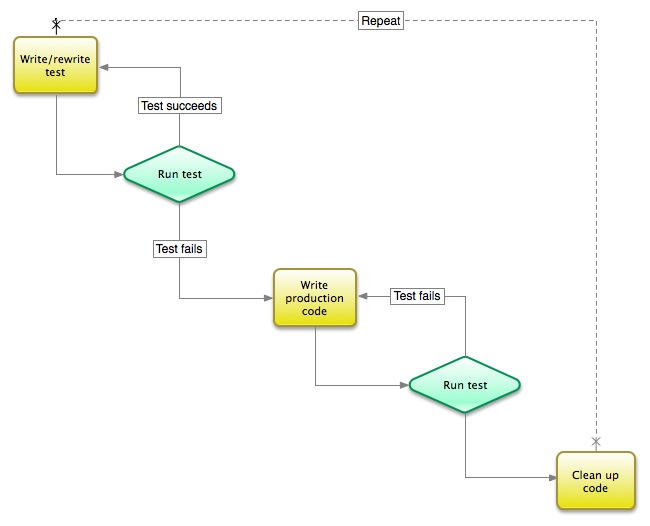
\includegraphics[width=0.9\textwidth]{figures/tdd-diagram-3.jpeg}
\caption{\label{fig:TDD1} TDD Cycle.}
\end{figure} 
     
\begin{enumerate}
\item Creation of a set of Unit tests that define the correct behavior of production code. Note: We must ensure that these tests initially fail. 
\item Creation of production code and subsequent checks to see if it passes  unit tests. Work on production code continues until all tests are passed.
\item Code is cleaned. Refactoring to increase readability and understanding of code.
\item More test cases may be added in order to ensure sufficient testing. The number of unit tests required for satisfactory testing is subject to the programmers judgment.
\end{enumerate}
     
\textbf{ Advantages of TDD are as follows:}
\begin{enumerate}
\item Increased reliability of code.
\item Programmers who write more tests are more productive.
\item Not just a validation of correctness: TDD also drives development by forcing the programmer to think strongly about how their code will be used. This leads to smaller, more focused classes, and cleaner interfaces.
\item Unit tests act as documentation: Testing functions are understandable examples of how the production code should be used.
\item TDD ensures consistent testing off all resources throughout the development of a piece of software.
\end{enumerate}

\subsection{Unit Tests}
Unit tests, as already mentioned, are tests that determine if individual units of source code are fit for use. It is important that unit tests are written very simply in order to ensure correctness (since there is no tests to ensure that the unit tests are correct). The following is a simple example of a test function and the corresponding production code it is intended to test.
      
\textbf{Unit Test:}
\begin{lstlisting}
void testAdd(){
  
  int expectedAnswer = 5;
  int answer = add(3 ,2);
  
  TEST_ASSERT(expectedAnswer == answer); //Check to see if output is as expected, and make record if it is not.
  
}
      
\end{lstlisting}
      
      \textbf{Production code (under test):}
      \begin{lstlisting}
int add(int a, int b){
  return a*b; //Obviously this will cause the test to fail
}
      \end{lstlisting}
      
      Obviously, the above test will fail because the function \emph{add()} has been implemented incorrectly. Using a Unit testing library such as CppTest we will recieve the following output:
      
      \begin{lstlisting}
FailTestSuite: 0/0, 0% correct in 0.000002 seconds
  Test:    testAdd
  Suite:   ExampleSuite
  File:    mytest.cpp
  Line:    9
  Message: "expectedAnswer == answer"
      \end{lstlisting}

%%================
\subsection{TDD Implementation in the OpenFCST}  
The unit testing structure that is implemented in OpenFCST is built using a library called CppTest.  CppTest is a portable, powerful, and simple unit testing framework for handling automated tests in C++. The focus lies on usability and extendability.

Several output formats, including simple text output, compiler-like output, and HTML can be produced. The tests suit is launched from the system builder class's \texttt{run\_tests()} function, see Figure \ref{fcstUnit}. Firstly, unit tests are run (which will test individual components of various classes), then system level tests. 
      
\FloatBarrier
\begin{figure}[h]
\begin{center}
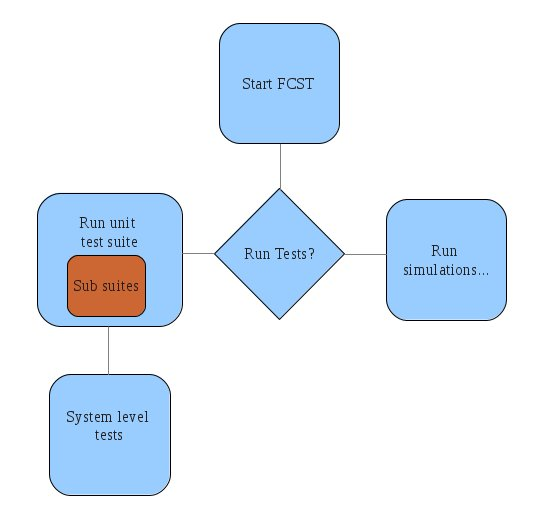
\includegraphics[width=0.7\textwidth]{figures/FCST_TDD.jpeg}
\caption{\label{fcstUnit} TDD illustration scheme.}
\end{center}
\end{figure}
\FloatBarrier

The operation is as follows.

The ``Run tests'' parameter is set in the main parameter file.

\begin{center}
\begin{lstlisting}
  set Run tests = true
\end{lstlisting}
\end{center}

The run test function in SimulatorBuilder is called, which in turn calls the OpenFCST testing suite.

\begin{center}
  \begin{lstlisting}
    void SimulatorBuilder<dim>::run_test()
    {	
	deallog << "==================Running Unit Tests===================" << std::endl;

	FcstTestSuite::run_tests();
	
	deallog << "================System Tests Complete==================" << std::endl;
  \end{lstlisting}
\end{center}

The OpenFCST test suite runs all of the unit testing suites that it is composed of (currently only the OpenFCST units testing suite)
\begin{center}
\begin{lstlisting}
bool FcstTestSuite::run_tests()
{
  Test::Suite ts;

  //add sub tests suites
  ts.add(std::auto_ptr<Test::Suite>(new FcstsUnitsTestSuite));
  ts.add(std::auto_ptr<Test::Suite>(new IonomerAgglomerate3Test));		

  Test::TextOutput output(Test::TextOutput::Verbose);
  return ts.run(output);

} 
\end{lstlisting}
\end{center}
Below is an example of an individual ''sub-testing'' suite. Each individual unit test is added to the test suite in the constructor and will be called individually when the .run() function is called.
\begin{center}
\begin{lstlisting}
#ifndef _FCST_UNITS_TESTSUITE
#define _FCST_UNITS_TESTSUITE

#include <cpptest.h>
#include "fcst_units.h"



class FcstsUnitsTestSuite: public Test::Suite
{
  public:
      FcstsUnitsTestSuite()
      {
	//Add a number of tests that will be called during Test::Suite.run()
	//Generic cases
	TEST_ADD(FcstsUnitsTestSuite::perBigToSmallTest);
	TEST_ADD(FcstsUnitsTestSuite::bigToSmallTest);
	TEST_ADD(FcstsUnitsTestSuite::perSmallToBig);
	TEST_ADD(FcstsUnitsTestSuite::smallToBig);
	  
	  //specific Cases
	TEST_ADD(FcstsUnitsTestSuite::btuToKwh);
	TEST_ADD(FcstsUnitsTestSuite::kwhToBtu);
      }
  protected:
      virtual void setup()     {} // setup resources... called before Test::Suite.run()
      virtual void tear_down() {} // remove resources...called after Test::Suite.run()    
      
  private:
	  //Generic cases
      void perBigToSmallTest();
      void bigToSmallTest();
      void perSmallToBig();
      void smallToBig();
      
      //Specific cases
      void btuToKwh();
      void kwhToBtu();
}; 

#endif
\end{lstlisting}
\end{center}

Below is an example of an individual unit test taken from the ``FcstsUnitsTestSuite'' test suite. It checks that the function \texttt{convert} correctly converts units of BTU to units of KJ.
\begin{center}
\begin{lstlisting}
void FcstsUnitsTestSuite::btuToKwh()
{
  TEST_ASSERT(Units::convert(1,Units::BTU_to_KJ) == 1.054);

}
\end{lstlisting}
\end{center}

%%================
\subsection{Implementing a new test suite}

If you would like to add a unit test suite for a class that you are creating, follow these steps:

\begin{enumerate}
 \item Create the class\_test.h and class\_test.cc files in the unit\_test folders (use the existing .h and .cc files as templates).
 \item Add an include statement to your new class\_test.h file in FCST\_TEST\_SUITE.h (under code comment "List of sub suites").
 \item In FCST\_TEST\_SUITE.cc, add your new test class in the run\_tests() function.
\end{enumerate}

If you would like your test to be able to see private variables inside the class that it is testing, you must add it as a friend to that class:
\begin{enumerate}
 \item Go to the header of the class you are testing (class.h).
 \item At the top of  the file (outside namespace scope), make a reference to your test class (e.g. "class nameOfTestClass;").
 \item In the class's declaration, write the friend statement above the public section (e.g. "friend class ::nameOfTestClass;").
\end{enumerate}

%%================    
\subsection{Refactoring}
Refactoring is a technique for restructuring existing code to improve it's readability and user understanding, without changing the behaviour of the code in any way. When refactoring code, a programmer looks for ``Bad Programming Smells'' and uses various methods to remove them. Code smells are not bugs, but weakness in code design that makes code difficult to understand and can lead to bugs being introduced into the code.
      
      Some examples of bad programming smells:
      \begin{enumerate}
       \item Duplicated code: identical or very similar code exists in more than one location.
       \item Long method: a method, function, or procedure that has grown too large or complicated.
       \item Inappropriate intimacy: a class that has dependencies on implementation details of another class.
       \item Too many parameters: a long list of parameters in a procedure or function make readability and code quality worse.
       \item Complex conditionals.
       \item Temporary variables and fields.
       \item Use of primatives rather than objects.
       \item Classes and functions with multiple responsibilities.
      \end{enumerate}

      The following is an example of code that exhibits bad smells (see if you can spot them):
      
      \begin{center}
      \begin{lstlisting}
void sendMessage(Message dataToSend, string phoneNumber, string networkOperator){
  
  string areaCode = "213";
  
  if (networkOperator == "Rogers"){
    string _phoneNumber = areaCode + "4" + phoneNumber;
    MessageBuffer b;

    for(int i=0; i < dataToSend.length(), i++)
      b.pack(dataToSend[i]);
    
    send(b, _phoneNumber)

  }
  else if(networkOperator == "Telus"){
  
    string _phoneNumber = areaCode + "9" + phoneNumber;
    MessageBuffer b;

    for(int i=0; i < dataToSend.length(), i++)
      b.pack(dataToSend[i]);
    
    send(b, _phoneNumber)
  
  }
}
      \end{lstlisting}
      \end{center}
      
      Bad smells include local data (the area codes should not be stored locally but should be the responsibility of another class such as PhoneBook), and duplicate code inside either if statement.
      The following code represents the above code refactored. The refactoring patterns extract method has been used to replace the code from within the for loop, the pattern extract data
      has been used to remove the local variables areaCode as well as the if statement comparisons. The result is code that is shorter, more easily understood, and more easily reused.
      
       \begin{center}
      \begin{lstlisting}
void sendMessage(Message dataToSend, string phoneNumber, string networkOperator){
  
  string fullPhoneNumer = PhoneBook::getAreaCode() + PhoneBook::getOperatorCode(networkOperator) + phoneNumber;
  MessageBuffer buffer = package(dataToSend);
  send(buffer, _phoneNumer)''
  
}

MessageBuffer package(Message dataToSend){
  MessageBuffer buffer
  
  for(int i=0; i < dataToSend.length(), i++)
    buffer.pack(dataToSend[i]);

  return buffer;
}
      \end{lstlisting}
      \end{center}
      
      Also note the change of variable names. The new names do a better job at describing their purpose.
      
%%================      
\subsection{Unit Standards}
OpenFCST uses centimetres, grams and seconds (CGS) units for most of its variables.

  
%%========================================================================================
%%========================================================================================
%%%===============================================================
%%===============================================================
\chapter{OpenFCST application testing suite using CTEST} \label{sec:CTest}
%%===============================================================
%% Author: Aslan Kosakian
%%===============================================================


CDash is an open source, web-based software testing server. CDash aggregates, analyzes and displays the results of software testing processes submitted from clients located around the world. CDash is available from \url{http://www.cdash.org/}, with info on installation and use at: \url{http://public.kitware.com/Wiki/CDash}. 

CDash however does not do any of the testing itself, it simply displays the results of tests run by another program produced by Kitware. This program is CTest, which is used to automate updating, configuring, building, testing, submitting results to a CDash dashboard system. It is normally used with the CMake system \url{http://www.cmake.org/}, a replacement for the Autotools and GNU make suite. In this manual, the setup of the dashboard is described, as well as the implementation of the test cases using CTest. 

This manual is written for openSUSE 13.1 and Ubuntu 14.04.

\section{Installing and configuring CDash}

\subsection{Prerequisites}\label{sec:Prerequisites}

Generally, only one CDash server is needed. In our case, it is a dashboard available at \url{http://129.128.14.197/CDash}. All testing machines, including the main server, \verb!secanell-srv01.mece.ualberta.ca!, report test results to that dashboard. If you only need to configure CTest on a machine so it runs tests and reports to \verb!secanell-srv01!, skip this chapter.

First, you need OpenFCST installed on your computer. If you already have OpenFCST, perform a clear installation, i.e. delete \verb!Build/! and \verb!Install/! folders before running the installation script.

Installation guide for CDash is available at \url{http://public.kitware.com/Wiki/CDash:Installation}. Before downloading CDash, you need to install Apache, MySQL and PHP 5 on your machine.

Although you can use terminal to install all the necessary packages, it is recommended to use YaST (openSUSE) or Synaptic (Ubuntu) to process a large number of packages. Complete list of required packages is given below.

\begin{enumerate}
 \item Apache2 and its supporting packages: 
 
\begin{center}
\begin{tabular}{|l|l|}
\hline
\textbf{openSUSE 13.1} & \textbf{Ubuntu 14.04}\\
\hline
\verb!apache2!            & \verb!apache2!     \\
\hline
\verb!apache2-devel!      & \verb!apache2-dev! \\
\hline
\verb!apache2-doc!        & \verb!apache2-doc! \\
\hline
                          & \verb!libapache2-mpm-itk! \\
\hline
\verb!apache2-prefork!	  & \verb!libapache2-mpm-prefork! \\
\hline
\verb!apache2-utils!      & \verb!apache2-utils! \\
\hline
\verb!apache2-mod\_php5!  & \verb!libapache2-mod-php5! \\
\hline
\verb!libapr-util1!       & \verb!libaprutil1! \\
\hline
\verb!libapr-util1-devel! & \verb!libaprutil1-dev! \\
\hline
\verb!libapr1!            & \verb!libapr1! \\
\hline
\verb!libapr1-devel!      & \verb!libapr1-dev! \\
\hline
\end{tabular}
\end{center}

\item If MySQL is not installed, install \verb!mariadb! package. MySQL will be installed as one of the dependencies. In Ubuntu, if, after the previous step, there is no "mysql" service (file) in \verb!/etc/init.d/!, install \verb!mysql-server!.

\bigskip

\textbf{Important:} Do not set password during installation of \verb!mysql-server!. If the password is set, you will not be able to open CDash in your browser. If you see the error saying "cannot connect to CDash on localhost using login root", run

\small \begin{lstlisting}
mysql admin -u root -p password
\end{lstlisting}\normalsize

\noindent and reset password to no password (hit enter when asked for a new password).\hfill$\blacksquare$

\bigskip

When done, install \verb!php5-mysql! in both systems.

\item CDash requires PHP 5.3 and higher. In both systems, install
\begin{enumerate}
 \item XSL module: \verb!php5-xsl!
 \item GD module: \verb!php5-gd!
 \item cURL module: \verb!php5-curl!
\end{enumerate}

\end{enumerate}

\subsection{Installation of CDash} \label{sec:Installation}

Usually, you need only one CDash server to report test results to. In our case, it is \verb!secanell-srv01! at \url{http://129.128.14.197/CDash}. By default, all CTest files in OpenFCST are configured to report to that dashboard as you will see later in this manual. However, if you need to install CDash on a different machine, follow the guides in this section.

Once Apache is installed, you can use \verb!subversion! or \verb!git! (might need to be installed) to get the latest release of CDash. When uploading a package such as this to Apache, it is normally put in the "htdocs" directory of the Apache file system. It is located in \verb!/srv/www/htdocs/! in openSUSE and \verb!/var/www/htdocs/! in Ubuntu. If there is no such folder, create it. Then, \verb!cd! to this directory and run

\small \begin{lstlisting}
svn co https://www.kitware.com/svn/CDash/Release-2-0-2 CDash
\end{lstlisting}\normalsize

\noindent or

\small \begin{lstlisting}
git clone https://github.com/Kitware/CDash.git CDash
\end{lstlisting}\normalsize

\noindent to download CDash files to a directory called "CDash". Note that the latest version of CDash is not available through \verb!svn!.

Open the permissions for this directory by using the following command as superuser:

\small \begin{lstlisting}
chmod -R 777 CDash 
\end{lstlisting}\normalsize

Next, add the Apache configuration file for CDash. Create a text file called "cdash.conf" in the directory\\

\noindent \verb!/etc/apache2/conf.d! (openSUSE)\\

\noindent or\\

\noindent \verb!/etc/apache2/conf-enabled/! (Ubuntu)\\

\noindent and add the following text:

\small \begin{lstlisting}
 <Directory PATH>
   Order allow,deny
   Allow from all
</Directory>
\end{lstlisting}\normalsize

\noindent where \verb!PATH! must be replaced by \verb!/srv/www/htdocs/CDash! in openSUSE and \verb!/var/www/htdocs/! in Ubuntu.

In \textbf{openSUSE}, open \verb!default-server.conf! in \verb!/etc/apache2/!, go to section marked ''<Directory ''/srv/www/htdocs''>'' and change ''Option'' flag from ''None'' to ''All''. Run \verb!vi /etc/sysconfig/apache2! and add ''php5'' to the line called ''APACHE MODULES''. Now start \verb!apache2! and \verb!mysql! services and make them run at boot:

\small \begin{lstlisting}
rcapache2 start
rcmysql start
chkconfig -a apache2
chkconfig -a mysql
chkconfig mysql on
\end{lstlisting}\normalsize

In \textbf{Ubuntu}, open ''000-default.conf'' in \verb!/etc/apache2/sites-enabled/! and add/edit the ''DocumentRoot'' line so it says ''DocumentRoot /var/www/CDash''. Start \verb!apache2! and \verb!mysql! services and make them run at boot:

\small \begin{lstlisting}
service apache2 start
service mysql start
apt-get install sysrv-rc-conf
sysv-rc-conf apache2 on
sysv-rc-conf mysql on
\end{lstlisting}\normalsize

Browsing \verb!http://computers-ip-address/CDash! should start CDash web-based configuration process. If you do not know your computer's IP address, run \verb!ifconfig! and look for ''inet addr'' line.

If any errors come up at this point, such as a black page or an error 403, access denied, then check the Apache error log in \verb!/var/log/apache2/!.

If any errors come up at this point, such as a black page or an error 403, access denied, then check the apache error log. This is usually located in /var/log/apache2/. Common errors are not setting the permissions correctly, or not having the necessary prerequisites. If an error shows up such as
\small \begin{lstlisting}
 Directory index forbidden by Options directive:
                                    /srv/www/htdocs/CDash/
\end{lstlisting}\normalsize
then try modifying the default-server.conf file located in /etc/apache2/. In the section marked 
\small \begin{lstlisting}
<Directory "/srv/www/htdocs"> 
\end{lstlisting}\normalsize
there is an Options flag likely with None beside it. Try changing this to All. (Note: changing this flag fixed the error, however changing it back to None then had no effect).

If there is a submission error saying "internal server error 500" (again, check the log files in \verb!/var/log/! for more info) then you are missing the \verb!php5-zlib! extension. Use yast to get the file, then modify the \verb!php.ini! file, located in \verb!/etc/php5/cli/!, so that it has the line ''extension=zlib.so'' (there is a section that has a number of similar lines, all commented out). You will then need to restart the computer. 

\subsection{Setting up a project} \label{sec:Setting up a project}

Before creating a project, the configuration file for CDash should be modified. This file is located in \\

\noindent \verb!/srv/www/htdocs/CDash/cdash/! (openSUSE)\\

\noindent or\\

\noindent \verb!/var/www/htdocs/CDash/cdash/! (Ubuntu)\\

\noindent and is called ''config.php''. This file should be left as it is. To make local modifications, copy and paste the contents of ''config.php'' into ''config.local.php''. Make all modifications in the local file. Delete section in the bottom called ''DO NOT EDIT AFTER THIS LINE'', or else the two files will be referencing each other. Now put your email address to the lines called ''\$CDASH\_EMAIL\_ADMIN=...'', ''\$CDASH\_EMAIL\_FROM=...'', and ''\$CDASH\_EMAIL\_REPLY=...''. If there are problems with loading CDash on the server, reports will be sent to you.

Another change that should be made is to limit how users are added. The default is to allow anybody to register themselves as a user on the website, if this is not wanted then the following line should be added to the file:

\small \begin{lstlisting}
$CDASH_NO_REGISTRATION = '1';
\end{lstlisting}\normalsize

\noindent To apply the changes, save the file and restart the server.

\subsubsection{Creating a project}

Again, if there are no errors, then navigating to \verb!http://localhost/CDash! should bring you to an installation screen where you will be asked for admin email address (which will also serve as the login) and a password. You can now log into the system and create a project. The first steps are to set the name, description and web links for the home of the code as well as documentation and bug tracker. 

Use the following links:

\begin{enumerate}
\item Home URL: \url{www.openfcst.mece.ualberta.ca/}
\item Bug Tracker URL: \url{https://bitbucket.org/ESDLab/openfcst/issues?status=new&status=open}
\item Documentation URL: \url{www.openfcst.mece.ualberta.ca/documentation.html}
\end{enumerate}

For the initial implementation of CDash nothing was changed in the testing, spam, clients or miscellaneous panel. For the email settings the 'Email redundant failures:' box was unchecked. This is because OpenFCST will always return a warning while linking with Dakota and will therefore always email about this warning. While nothing is changed in the miscellaneous panel, it does give the option to download a file called "CTestConfig.cmake". This is a file that will be used later when setting up the testing on the computer, so download this file. 

\subsection{Recovering CDash after OS update}

Each time you update your Linux distribution, i.e. upgrade your operating system, you will need to first backup all the files related to CDash and then recover them after the system is updated. If you are lucky, MySQL and Apache2 will still be working. Otherwise, install them again.

If you have not backed up all packages required for OpenFCST (including \verb!git!), install them again and reinstall OpenFCST.

On this stage, if you go to \verb!http://localhost/CDash!, it will automatically redirect you to the installation page and show a connection error. Delete local CDash configuration file, \verb!config.local.php!, and reload the page. This will start a fresh web-based installation of CDash. When asked to enter email and password, use your old ones. Now you will see a completely empty CDash page with no submissions and no project. Create a new local configuration file, edit it, save it, and create a new project in CDash following instruction in this manual. Note that you need to use the same name for the project as you used before. We call a project on the main server ''FCST''. Restart both Apache2 and MySQL services.

You will also need to install a new cron job for running the tests.

\subsection{Using the website}

The project can now be created. Any settings made here can be changed later, apart from the name. They can be changed by going to the administration panel for the dashboard. Note that the website can support multiple dashboards and a user can change the settings for any dashboard they are admin for. Choose the dashboard you wish to change (this can be done by going to the ''My CDash'' link in the top left hand corner and then choosing the dashboard) then hover the mouse over the administration button. The settings mentioned in the previous paragraph can be changed in the ''project'' section of the drop down menu that will appear. Other users can be added by going to the ''users'' section. Note that this will add users to this dashboard only. This panel should not be used to add users to the website as the ''Register User'' section is incomplete. See the next section for more information on this. 

\subsubsection{Adding users}

To add new users, login as admin and click on ''My CDash''. The admin user has a lot more options here than a normal user (see example on figure \ref{fig:my_cdash}), including the options in the administration panel mentioned earlier. 

\begin{figure}[!h]
\centering
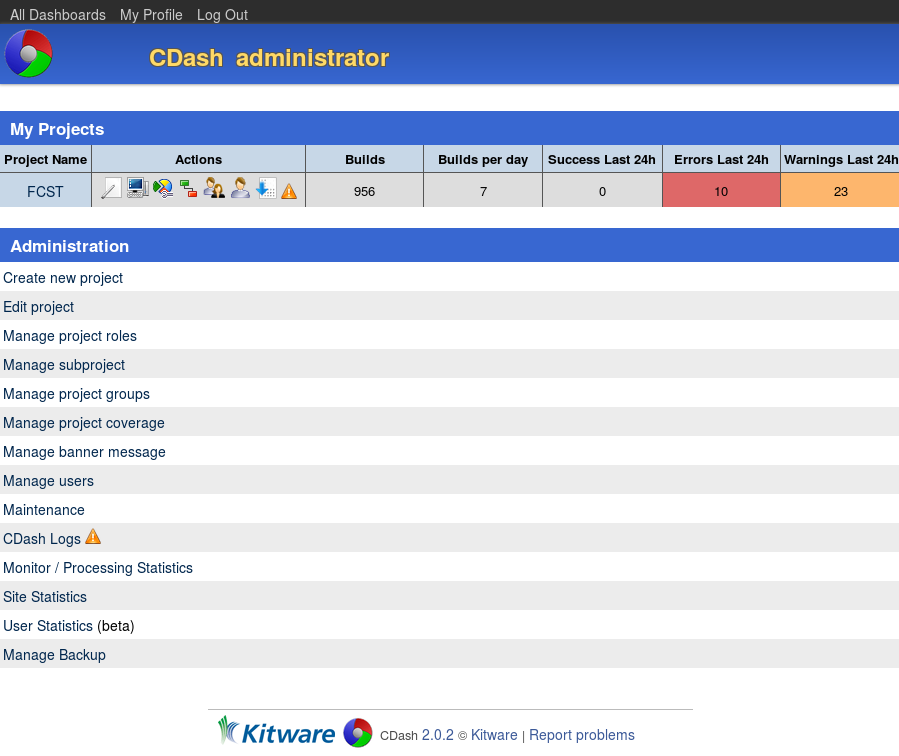
\includegraphics[width=1\textwidth]{figures/CDash/my_cdash.png}
\caption{''My CDash'' example page for an administrator}
\label{fig:my_cdash}
\end{figure}

Click on ''Manage users'', where new users can be added. Create the new user here and then go to the ''Project Roles'' page from the ''My CDash'' page. Here you can assign users to a project and also give their name repository name. CDash will use this during the testing process to email the users who last committed code if it crashes. The role of the user can also be assigned. The project administrator is in charge of the code and will always get emails if the code crashes or if there are errors in submitting results to the dashboard. Site maintainers are users of the code who also run and submit tests from their computers. They will be responsible for making sure that the code they are working on is running correctly and will be emailed if the tests they run are failing. This is achieved by having the user submit a test to the dashboard and then ''claiming the site''. CDash will keep a record of the 
computers that are performing tests and if a user claims a site they are responsible for the tests from that site. Normal users are users that simply use the code and want to keep track of code. 

Each user can have their own settings for how they are informed about the success of their tests. Going back to the ''My CDash'' page, under ''My Projects'' is a list of the dashboards the user is registered to. Under actions, the user can click the page icon to change their personal settings, such as email settings, role in a project and repository credential(s). Clicking the small computer icon will bring up a list of computers that have submitted tests to the dashboard, allowing the user to claim sites. 

There is one more useful section on the ''My CDash'' page for administrators, the ''CDash Logs''. If there are parts of the site that are not working, this is a useful place to look. It also logs other information such which users were emailed if a test has failed. 

\subsubsection{The CDash interface}

If the project has just been created, then project home page should now be available, with 5 lines saying ''no Nightly builds'' etc. This is the main page of the project, where all the information about the testing will be seen. It can be accessed by going to ''My CDash'' and choosing the dashboard from the ''My Projects'' section. An example is given on figure \ref{fig:project_page}.

\begin{figure}[!h]
\centering
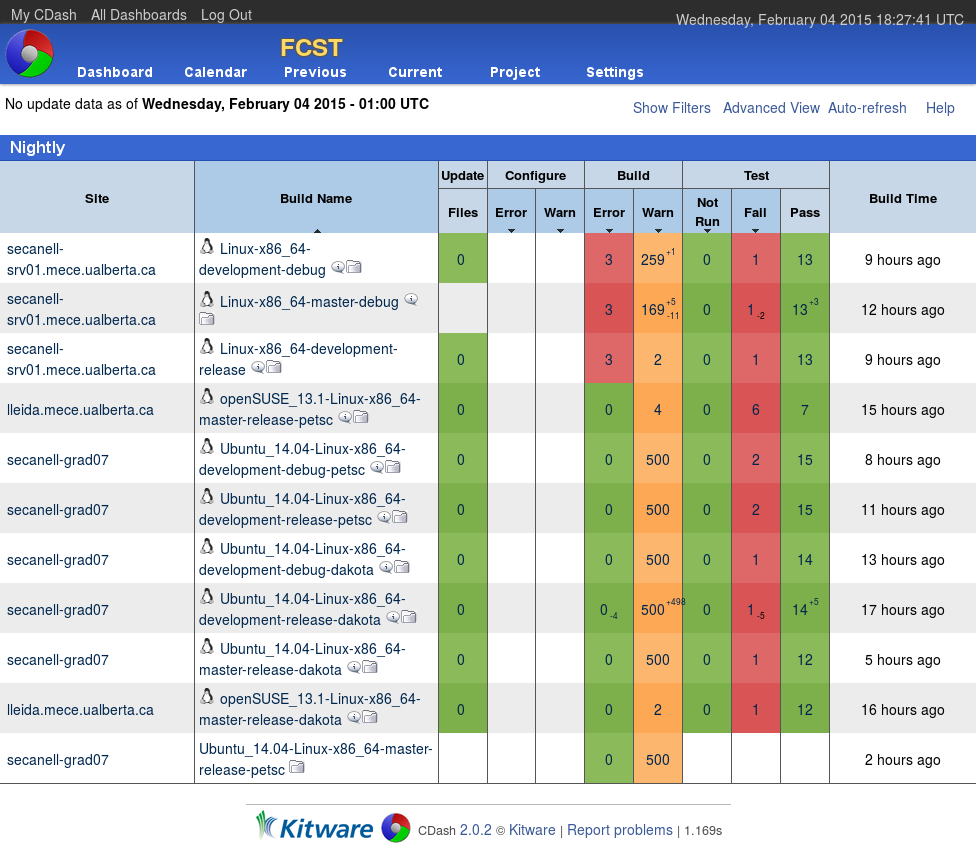
\includegraphics[width=1\textwidth]{figures/CDash/cdash.png}
\caption{Project's main page example}
\label{fig:project_page}
\end{figure}

On the project's main page, we can see the information given by CDash about test results for various builds and testing machines. From the dashboard, you know on which machine the tests were run (''Site''), what were the operating system and OpenFCST build parameters (''Build Name''), and detailed information on test results. A normal test run by CTest is to automatically update the code using \verb!git!, configure the code, build the code and then run tests to ensure that the code is behaving as expected.

In this test, performed on the 4th of February 2015, a testing sequence was run on three different machines, \verb!secanell-srv01.mece.ualberta.ca! (our main server; openSUSE~12.3), \verb!lleida.mece.ualberta.ca! (openSUSE~13.1), and \verb!secanell-grad07! (Ubuntu~14.04). If there are any locally modified files, CDash gives a warning in ''Configure'' section, and gives an error if there are conflicts. Usually, if the tests are being run on code that is located on the testing machine, there should not be any issues with the update process as nobody will be working on the code on those computers.

The ''Build'' section returns errors and warnings that appeared on the OpenFCST building stage. The ''Test'' section shows number of tests that were failed or passed. Each of the numbers shown can be clicked on to give more information. For example, if part of the build returns a warning as it did in the example above, clicking on the number will show the page given on figure \ref{fig:cdash_warning}.

\begin{figure}[!h]
\centering
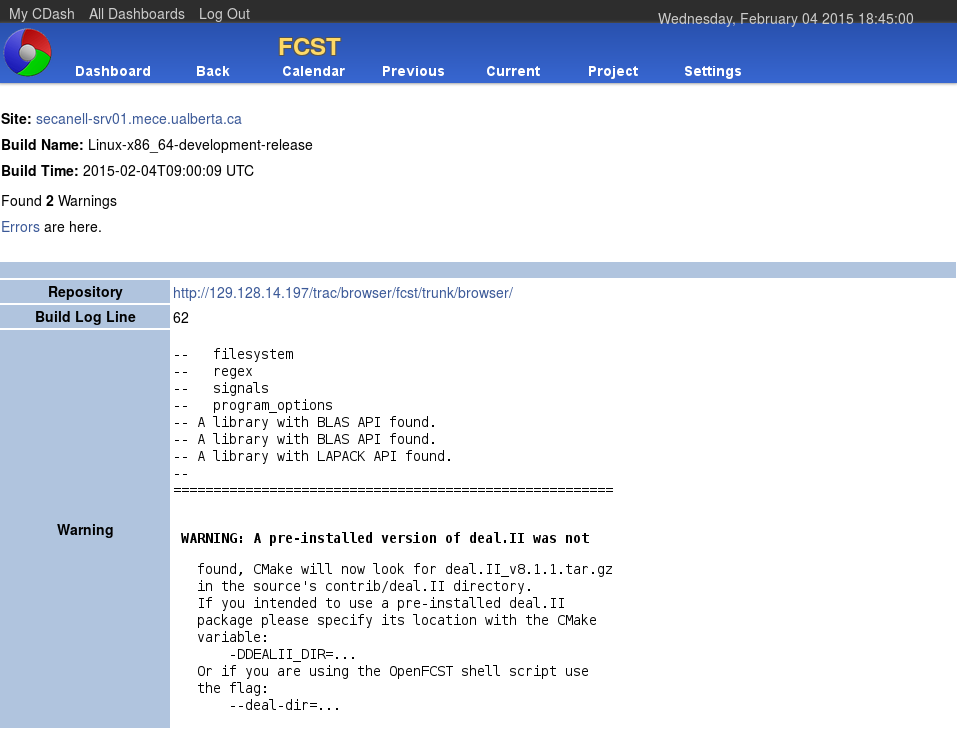
\includegraphics[width=1\textwidth]{figures/CDash/cdash_warning.png}
\caption{Example of the warning information page}
\label{fig:cdash_warning}
\end{figure}

\section{Configuring CTest}

\subsection{Testing your code in your local revision}
Before committing any changes made in your local revision, you should make sure that your working copy  passess provided tests. You can test your working copy of OpenFCST by typing the following in the command line in the OpenFCST main folder:
\begin{lstlisting}
$./run_tests
\end{lstlisting}

All test cases that have been programmed will be executed. Test summary output will be written to tests\_summary.log, and all OpenFCST output will be written to tests\_output.log. At present there are several tests provided, for various applications and the unit testing suite. 

\subsection{Setting up a CTest testing suite}\label{sec:setting_up_CTest}

When setting up a test using CTest, the normal procedure is to use the CMake suite of tools to configure and compile the code. Setting up CTest is then a very simple addition to this process.  To do this a ''steering'' file needs to be created, which will extract information about the computer and implement the commands for the update, configure, build and testing of the code. Setting up this file, called \verb!nightly_tests.cmake!, will be described by going through the file created for one of the testing machines, as well as its contributing files and associated processes.

To simply install a nightly test system on Linux, one can follow the following quick steps:
\begin{enumerate}
 \item Copy \verb!nightly_tests! \verb!.sh! and \verb!.cmake! to the OpenFCST root folder (where the install scripts reside).
 \item Edit the address line in that script to cd to OpenFCST root folder. Use the full address, e.g. \verb!/home/cdash/openfcst/!.
 \item Set up \verb!git! user credential caching as follows:
  \subitem Clear you credentials: \verb!git config credential.helper clear!
  \subitem Set the credentials to store: \verb!git config credential.helper store!
  \subitem Finally \verb!git pull! and enter your credentials
  \subitem More info at  \url{http://tinyurl.com/git-password}
\end{enumerate}

\subsubsection{The main steering file}

Two similar testing systems are supplied with OpenFCST. The \verb!run_tests! script will run test cases and report results directly back to the user. The nightly testing system is more thorough: it will update, build, install, and test the code for multiple branches and build modes, then finally report testing results to a CDash server which displays the results to other developers.

Here we will go through the nightly tests steering file, \verb!nightly_tests.cmake!, section by section.

\small \begin{lstlisting}
# -----------------------------------------------------------  
# -- Get environment
# -----------------------------------------------------------  

## -- Set hostname
## --------------------------
find_program(HOSTNAME_CMD NAMES hostname)
exec_program(${HOSTNAME_CMD} ARGS OUTPUT_VARIABLE HOSTNAME)

#Name of this computer
set(CTEST_SITE                          "${HOSTNAME}")

## -- Set site / build name
## --------------------------

find_program(UNAME NAMES uname)
macro(getuname name flag)
  exec_program("${UNAME}" ARGS "${flag}" OUTPUT_VARIABLE
                                               "${name}")
endmacro(getuname)

getuname(osname -s)
getuname(osrel  -r)
getuname(cpu    -m)


set(MODEL                               "Nightly")

## -- SVN command
## ----------------
find_program(CTEST_GIT_COMMAND NAMES git)

## -- make command
## -----------------
find_program(MAKE NAMES make)
\end{lstlisting}\normalsize

The first section, ''get environment'', contains commands that will find the name and some of the specifications of the computer, as well as the commands for the call to \verb!CMake! and \verb!git!. Here we also give the type of tests we are running. In this case we are running ''Nightly'' tests, so CDash will display the results from this build in the nightly section of the interface. Other choices are ''Continuous'' and ''Experimental''.

The file now gets specific to the tests that we are performing, e.g. defines a path to other CTest files (read on):

\small \begin{lstlisting}
# -----------------------------------------------------------  
# -- build specificFCST
# -----------------------------------------------------------  

## -- DashBoard Root
set(CTEST_DASHBOARD_ROOT        ${CMAKE_CURRENT_LIST_DIR})

## -- SRC Dir
set(CTEST_SOURCE_DIRECTORY     "${CTEST_DASHBOARD_ROOT}/
                                             Install/test")

## -- BIN Dir                                            
set(CTEST_BINARY_DIRECTORY     "${CTEST_SOURCE_DIRECTORY}/
                                build-${CTEST_BUILD_NAME}")
\end{lstlisting}\normalsize

Next, we set some directories. The root folder is OpenFCST root directory, where the install scripts, \verb!src/!, \verb!Install/! and \verb!Build/! folders exist. The source folder is where additional \verb!.cmake! files exist, as well as the individual test cases. The binary directory is where we will store the results from the test we are going to run. 

Pretty much all the following code does is setting an update command, defining a directory for CTest custom files (later in this manual).

\small \begin{lstlisting}
# -----------------------------------------------------------  
# -- commands
# -----------------------------------------------------------  

## -- Update Command
set(CTEST_UPDATE_COMMAND        "${CTEST_GIT_COMMAND}")

# -----------------------------------------------------------  
# -- Configure CTest
# -----------------------------------------------------------  

## -- read CTestCustom.cmake file
ctest_read_custom_files("${CTEST_SOURCE_DIRECTORY}")

# -----------------------------------------------------------  
# -- Settings
# -----------------------------------------------------------  

## -- Process timeout in seconds
set(CTEST_TEST_TIMEOUT           "14400")

## -- Set output to english
set( $ENV{LC_MESSAGES}      "en_EN" )

\end{lstlisting}\normalsize

Then, we specify Bitbucket branches of OpenFCST that we are going to test, build modes, build flags, and the name of the operating system. Note that \verb!osname! variable that we declared earlier does not contain Linux distribution name and its version, e.g. ''openSUSE 13.1'' or ''Ubuntu 14.04''. On each testing machine, you need to modify \verb!DISTR_NAME! declaration line in this file.

\small \begin{lstlisting}
# -----------------------------------------------------------  
# -- Run CTest
# -----------------------------------------------------------  

##----Remove comments made using a single hash key in order
##----to get CTest to test that component.

 ############################################################
 #####################                  #####################
 ##################### Testing sequence #####################
 #####################                  #####################
 ############################################################ 

 set(GIT_BRANCHES "development" "master")
 set(BUILD_MODES "release" "debug")
 set(BUILD_FLAGS "dakota" "petsc")
 set(DISTR_NAME "openSUSE_13.1")

\end{lstlisting}\normalsize

After that, we create a file (rewrite if it exists) \verb!config.txt! in \verb!/Install/test! that contains certain flags. You will see later that another \verb!.cmake! file, specifically \verb!CTestTestfile.cmake!, reads this text file and enables/disables some of the test cases depending on what flag was written to \verb!config.txt!.

\small \begin{lstlisting}
 ## WRITE: -- First, turn all options off.

 file(WRITE ${CTEST_DASHBOARD_ROOT}/Install/test/config.txt
                       "List of current build flags:" "\n")
 file(APPEND ${CTEST_DASHBOARD_ROOT}/Install/test/config.txt
                    "PETScOFF" "\n") # Turn PETSc option off
 file(APPEND ${CTEST_DASHBOARD_ROOT}/Install/test/config.txt
                  "DAKOTAOFF" "\n") # Turn Dakota option off

 ## WRITE: -- End
\end{lstlisting}\normalsize

Finally, in several \verb!FOREACH! loops, we ckeckout branches (update local files), build OpenFCST, run tests, and submit the results to CDash. In this example, we test the following builds:

\begin{itemize}
\item master-release-dakota;
\item master-release-petsc;
\item development-release-dakota;
\item development-release-petsc;
\item development-debug-dakota;
\item development-debug-petsc,
\end{itemize}

\noindent which correspond to 

\begin{itemize}
\item OpenFCST version from ''master'' branch compiled in ''release'' mode with \verb!--with-dakota! flag;
\item OpenFCST version from ''master'' branch compiled in ''release'' mode with \verb!--with-petsc! flag;
\item OpenFCST version from ''development'' branch compiled in ''release'' mode with \verb!--with-dakota! flag;
\item OpenFCST version from ''development'' branch compiled in ''release'' mode with \verb!--with-petsc! flag;
\item OpenFCST version from ''development'' branch compiled in ''debug'' mode with \verb!--with-dakota! flag;
\item OpenFCST version from ''development'' branch compiled in ''debug'' mode with \verb!--with-petsc! flag.
\end{itemize}

For each build, we rewrite \verb!config.txt! to turn on/off Dakota- and PETSc-specific tests.

You might want to change the number of cores used for building OpenFCST depending on specifications of your machine. To do that, modify \verb!--cores! value in each of  \verb!set(CTEST_BUILD_COMMAND ...)! lines.

\small \begin{lstlisting}
 FOREACH(GIT_BRANCH ${GIT_BRANCHES})

 FOREACH(BUILD_FLAG ${BUILD_FLAGS})

  IF(GIT_BRANCH STREQUAL "master")

   set(BUILD_MODE "release")

   IF(BUILD_FLAG STREQUAL "dakota")
   
    file(WRITE
    ${CTEST_DASHBOARD_ROOT}/Install/test/config.txt
    "List of current build flags:" "\n")
    
    file(APPEND
    ${CTEST_DASHBOARD_ROOT}/Install/test/config.txt
    "PETScOFF" "\n")
    
    file(APPEND
    ${CTEST_DASHBOARD_ROOT}/Install/test/config.txt
    "DAKOTAON" "\n")
     
    set(CTEST_BUILD_COMMAND "./openFCST_install --cores=4
                                          --with-dakota")
                                          
   ELSEIF(BUILD_FLAG STREQUAL "petsc")
   
    file(WRITE
    ${CTEST_DASHBOARD_ROOT}/Install/test/config.txt
    "List of current build flags:" "\n")
    
    file(APPEND
    ${CTEST_DASHBOARD_ROOT}/Install/test/config.txt
    "PETScON" "\n")
    
    file(APPEND
    ${CTEST_DASHBOARD_ROOT}/Install/test/config.txt
    "DAKOTAOFF" "\n")
    
    set(CTEST_BUILD_COMMAND "./openFCST_install --cores=4
                                           --with-petsc")
                                           
   ENDIF()

    ## -- Checkout the branch
    execute_process (COMMAND ${CTEST_GIT_COMMAND} checkout
                                            ${GIT_BRANCH})
    set(CTEST_BUILD_NAME
    "${DISTR_NAME}-${osname}-${cpu}-${GIT_BRANCH}-
                             ${BUILD_MODE}-${BUILD_FLAG}")

    message(" -- Start dashboard ${MODEL} - ${GIT_BRANCH}
    - ${CTEST_BUILD_NAME} - ${BUILD_MODE} - ${BUILD_FLAG}
                                                     --")
                                                       
    ctest_start(${MODEL} TRACK ${MODEL})

    ## -- Update
    message(" -- Update ${MODEL} - ${GIT_BRANCH}
    - ${CTEST_BUILD_NAME} - ${BUILD_MODE}
                             -${BUILD_FLAG} --")
    ctest_update(
    SOURCE "${CTEST_DASHBOARD_ROOT}" RETURN_VALUE res)

    # -- BUILD, build the whole project
    message(" -- Build ${MODEL} - ${GIT_BRANCH}
    - ${CTEST_BUILD_NAME} - ${BUILD_MODE} -${BUILD_FLAG}
                                                    --")
    ctest_build(    BUILD  "${CTEST_DASHBOARD_ROOT}"
                                   RETURN_VALUE res)

    ## -- TEST
    message(" -- Test ${MODEL} - ${GIT_BRANCH}
    - ${CTEST_BUILD_NAME} -${BUILD_MODE} -${BUILD_FLAG}
                                                   --")
    ctest_test(     BUILD  "${CTEST_SOURCE_DIRECTORY}"
                                      RETURN_VALUE res)

    ## -- SUBMIT
    message(" -- Submit ${MODEL} - ${GIT_BRANCH}
    - ${CTEST_BUILD_NAME} -${BUILD_MODE} -${BUILD_FLAG}
                                                   --")
    ctest_submit(                     RETURN_VALUE res)

    message(" -- Finished ${MODEL}  - ${GIT_BRANCH}
    - ${CTEST_BUILD_NAME} -${BUILD_MODE} -${BUILD_FLAG}
                                                   --")

   ELSEIF(GIT_BRANCH STREQUAL "development")

    FOREACH(BUILD_MODE ${BUILD_MODES})

     IF(BUILD_FLAG STREQUAL "dakota")

      file(WRITE
      ${CTEST_DASHBOARD_ROOT}/Install/test/config.txt
                 "List of current build flags:" "\n")
                 
      file(APPEND
      ${CTEST_DASHBOARD_ROOT}/Install/test/config.txt
                                     "PETScOFF" "\n")   
                                        
      file(APPEND
      ${CTEST_DASHBOARD_ROOT}/Install/test/config.txt
                                     "DAKOTAON" "\n")
                                     

        IF(BUILD_MODE STREQUAL "release")
         set(CTEST_BUILD_COMMAND  "./openFCST_install
                           --cores=4  --with-dakota")
        ELSEIF(BUILD_MODE STREQUAL "debug")
         set(CTEST_BUILD_COMMAND  "./openFCST_install
          --cores=4  --with-dakota --openfcst-debug")
        ENDIF()

       ELSEIF(BUILD_FLAG STREQUAL "petsc")

        file(WRITE
        ${CTEST_DASHBOARD_ROOT}/Install/test/config.txt
                   "List of current build flags:" "\n")
                   
        file(APPEND
        ${CTEST_DASHBOARD_ROOT}/Install/test/config.txt
                                        "PETScON" "\n")
        file(APPEND
        ${CTEST_DASHBOARD_ROOT}/Install/test/config.txt
                                      "DAKOTAOFF" "\n")

        IF(BUILD_MODE STREQUAL "release")
          set(CTEST_BUILD_COMMAND  "./openFCST_install
                             --cores=4  --with-petsc")
        ELSEIF(BUILD_MODE STREQUAL "debug")
          set(CTEST_BUILD_COMMAND   "./openFCST_install
             --cores=4  --with-petsc --openfcst-debug")
        ENDIF()

       ENDIF()

       ## -- Checkout the branch
       execute_process (COMMAND ${CTEST_GIT_COMMAND} checkout
                                               ${GIT_BRANCH})
       set(CTEST_BUILD_NAME
       "${DISTR_NAME}-${osname}-${cpu}-${GIT_BRANCH}-
                                ${BUILD_MODE}-${BUILD_FLAG}")

       message(" -- Start dashboard ${MODEL} - ${GIT_BRANCH}
       - ${CTEST_BUILD_NAME} - ${BUILD_MODE} - ${BUILD_FLAG}
                                                     --")
                                                       
       ctest_start(${MODEL} TRACK ${MODEL})

       ## -- Update
       message(" -- Update ${MODEL} - ${GIT_BRANCH}
       - ${CTEST_BUILD_NAME} - ${BUILD_MODE}
                                -${BUILD_FLAG} --")
       ctest_update(
       SOURCE "${CTEST_DASHBOARD_ROOT}" RETURN_VALUE res)

       # -- BUILD, build the whole project
       message(" -- Build ${MODEL} - ${GIT_BRANCH}
       - ${CTEST_BUILD_NAME} - ${BUILD_MODE} -${BUILD_FLAG}
                                                       --")
      ctest_build(    BUILD  "${CTEST_DASHBOARD_ROOT}"
                                      RETURN_VALUE res)
 
       ## -- TEST
       message(" -- Test ${MODEL} - ${GIT_BRANCH}
       - ${CTEST_BUILD_NAME} -${BUILD_MODE} -${BUILD_FLAG}
                                                      --")
       ctest_test(     BUILD  "${CTEST_SOURCE_DIRECTORY}"
                                         RETURN_VALUE res)

       ## -- SUBMIT
       message(" -- Submit ${MODEL} - ${GIT_BRANCH}
       - ${CTEST_BUILD_NAME} -${BUILD_MODE} -${BUILD_FLAG}
                                                      --")
       ctest_submit(                     RETURN_VALUE res)

       message(" -- Finished ${MODEL}  - ${GIT_BRANCH}
       - ${CTEST_BUILD_NAME} -${BUILD_MODE} -${BUILD_FLAG}
                                                      --")

     ENDFOREACH()
   ENDIF()

 ENDFOREACH() # BUILD_FLAG

    file(WRITE
    ${CTEST_DASHBOARD_ROOT}/Install/test/config.txt
               "List of current build flags:" "\n")
    
    file(APPEND
    ${CTEST_DASHBOARD_ROOT}/Install/test/config.txt
                                   "PETScOFF" "\n")
                                   
    file(APPEND
    ${CTEST_DASHBOARD_ROOT}/Install/test/config.txt
                                  "DAKOTAOFF" "\n")

 ENDFOREACH() # GIT_BRANCH
\end{lstlisting}\normalsize

This completes the steering file.

Note that the test command was not specified in the steering file. This is actually done in another file which will be discussed next.

\subsubsection{Contributing files}

There are three contributing files that are needed by CTest. Information on the three files can be found at the following page:
\url{http://www.vtk.org/Wiki/CTest:Using_CTEST_and_CDASH_without_CMAKE}.

The first is the \verb!CTestCustom.cmake! file that is used to customize the testing process:

\small \begin{lstlisting}
set(CTEST_CUSTOM_MAXIMUM_NUMBER_OF_WARNINGS "500" )
set(CTEST_CUSTOM_MAXIMUM_FAILED_TEST_OUTPUT_SIZE "100000" )
set(CTEST_CUSTOM_MAXIMUM_PASSED_TEST_OUTPUT_SIZE "100000" )
\end{lstlisting}\normalsize

Here we limit the number of warnings that CTest will report and we also limit the size of the output of the results file. More options are given on the webpage mentioned above.

The next file is the \verb!CTestConfig.cmake! file which gives CTest the information about the CDash website:

\small \begin{lstlisting}
set(CTEST_PROJECT_NAME "FCST")
set(CTEST_NIGHTLY_START_TIME "01:00:00 UTC")

set(CTEST_DROP_METHOD "http")
set(CTEST_DROP_SITE "129.128.14.197")
set(CTEST_DROP_LOCATION "/CDash/submit.php?project=FCST")
set(CTEST_DROP_SITE_CDASH TRUE)
\end{lstlisting}\normalsize

Note that the time set is just a time stamp for CDash. The actual time when tests are run is set using Cron (read on).

The last CTest file is \verb!CTestTestfile.cmake!. This is where we specify the tests we want to run. This is done using the following command:

\small \begin{lstlisting}
ADD_TEST(app_cathode "test_cases/app_cathode_case.sh")
\end{lstlisting}\normalsize

All the tests are added with a simple command like that one.

The command contains the name of the test, \verb!app_cathode!, and the test file to be executed. Note that the test file is a bash script that actually runs the code. This script will run the code and then compare the results to the expected results file:

\small \begin{lstlisting}
cd ../data/cathode/testing
rm polarization_curve.dat
../../../bin/fuel_cell-2d.bin main_app_cathode_test.prm

if [ "${PIPESTATUS[0]}" != "0" ]; then
	echo  2>&1 | tee tests_summary.log
	echo  "Results summary from the app_cathode test:"
	             2>&1 | tee --append tests_summary.log
	echo  2>&1 | tee --append tests_summary.log
	echo "-----" 2>&1 | tee --append tests_summary.log
	echo "The simulation did not run correctly. Please
	review the tests_output.log file  "  2>&1 | tee
	                        --append tests_summary.log
	echo "-----" 2>&1 | tee --append tests_summary.log
	echo  2>&1 | tee --append tests_summary.log
	cat tests_summary.log >> ../../../tests_summary.log 
  exit 2
else
	../../../test/csvPoleCurveCompare.py
	            polarization_curve.dat test_results.dat
	if [ "${PIPESTATUS[0]}" != "0" ]; then
		echo  2>&1 | tee tests_summary.log
		echo  "Results summary from the app_cathode
		test:" 2>&1 | tee --append
		                          tests_summary.log
		echo 2>&1 | tee --append
		                          tests_summary.log
		echo "--" 2>&1 | tee --append
		                          tests_summary.log
		echo "Results from the test do not match
		expected results" 2>&1 | tee --append
		                          tests_summary.log
		echo "Please check the results in
		polarization_curve.dat against that of
		test_results.dat" 2>&1 | tee --append
		                          tests_summary.log
		echo "--" 2>&1 | tee --append
		                          tests_summary.log
		echo 2>&1 | tee --append
		                          tests_summary.log
		cat tests_summary.log >>
		                 ../../../tests_summary.log 
		exit 2
	else 
		echo  2>&1 | tee tests_summary.log
		echo  "Results summary from the app_cathode
		   test:" 2>&1 | tee --append
		                          tests_summary.log
		echo 2>&1 | tee --append tests_summary.log
		echo "--" 2>&1 | tee --append
		                          tests_summary.log
		echo "Results from the test match expected
		 results" 2>&1 | tee --append
		                          tests_summary.log
		echo  "-" 2>&1 | tee --append
		                          tests_summary.log
		echo 2>&1 | tee --append tests_summary.log
		cat tests_summary.log >>
		                 ../../../tests_summary.log 
		exit 0
	fi
fi
\end{lstlisting}\normalsize

The test case will run the code with the \verb!app_cathode! test case file. If anything goes wrong, the script will save error information to \verb!tests_summary.log! file.

It is worth to note how \verb!CTestTestfile.cmake! interacts with \verb!config.txt! file that we mentioned when we were discussing the steering file.

The \verb!CTestTestfile.cmake! version located in \verb!src/! folder of OpenFCST contains the following line:

\small \begin{lstlisting}
file(STRINGS @CMAKE_INSTALL_PREFIX@/test/config.txt FLAGS)
\end{lstlisting}\normalsize

When OpenFCST is being installed, it replaces \verb!@CMAKE_INSTALL_PREFIX@! with actual path to \verb!Install/! directory. Note that, after the installation process, you will have two sets of CTest configuration files: in \verb!Install/! folder and in \verb!src/! folder. The tests are run in \verb!Install/! folder.

All lines from \verb!config.txt! are read to the \verb!FLAGS! string list variable. Then, the commands

\small \begin{lstlisting}
list(FIND FLAGS "PETScON" PETSc_FLAG)
list(FIND FLAGS "DAKOTAON" Dakota_FLAG)
\end{lstlisting}\normalsize

\noindent check if certain flags were set on. In general, \verb!list(FIND list value variable)! returns index of the element in the \verb!list! through \verb!variable! if the \verb!value! was found or -1 if it was not. So we use this fact to enable/disable our package-specific tests like those which need PETSc or Dakota:

\small \begin{lstlisting}
## -- Parallel tests
IF(PETSc_FLAG GREATER -1)
  ADD_TEST(app_cathode_parallel
                 "test_cases/app_cathode_parallel_case.sh")
  ADD_TEST(app_diffusion_3D_parallel
                 "test_cases/app_diffusion_3D_parallel.sh")
ENDIF() # PETSc_FLAG

# -- Dakota integration test:
IF(Dakota_FLAG GREATER -1)
  ADD_TEST(dakota_parametric
                   "test_cases/app_cathode_dakota_case.sh")
ENDIF() # Dakota_FLAG
\end{lstlisting}\normalsize

\subsubsection{Setting an automatic nightly testing}

To make the tests run every night, cron is used. Cron is a program that allows a user to schedule programs to run at a set time automatically. The script and time and day it should be run at are specified in a file created by cron. The bash script we use is called \verb!nightly_tests.sh! and it is packaged in a zip file inside the \verb!test/! folder. The script sets some environment variables required to build OpenFCST, cleans OpenFCST and its contribs, and then launches the CTest steering file. After unpacking files from the archive as it was described in subsection \ref{sec:setting_up_CTest},  add a \verb!Cron! job to execute \verb!nightly_tests.sh! nightly. Use \verb!crontab -e!. The line you add should look like this:\\

\verb!0 02 * * * /bin/bash /home/cdash/openfcst/nightly_tests.sh!\\
 
The address of the script has to be full.

This cron job will run \verb!nightly_tests.sh! every night at 2 a.m. local time. For more info on how to configure Cron jobs, go to \url{http://tinyurl.com/crontab-howto}.

This completes the setup of the testing suite.

%%===============================================================
%%===============================================================
%%===============================================================
%%===============================================================
%%===============================================================
%%===============================================================
%%%===============================================================
%%===============================================================
\chapter{Useful Programming Tips}
%%===============================================================
%%===============================================================
%% Author: 
%%===============================================================
%%===============================================================
if you would like to count lines of code use the following two commands for the .h and .cc files:
\begin{lstlisting}
$find . -name '*.h' | xargs wc -l
$find . -name '*.cc' | xargs wc -l
\end{lstlisting}
Then, add all the lines. As of September 11, 2013 the code has 157,801 lines of code (including comments and empty lines).

%%===============================================================
\section{Memory Leak Detection}
%%===============================================================

Despite taking all precautions to avoid memory leaks, it is still a possibility. It is recommended that developers make use of the program Valgrind.  It is a freely available, open-source software, and can be found in the software packaged with most Linux distributions.  Valgrind checks memory operations of any program, without having to modify the program in any way.  It will typically make the program run 20-50 times slower than normal.  To run, simply call \texttt{valgrind --options} before your normal program call.  E.g.
\begin{lstlisting}
valgrind --leak-check=full --show-below-main=no --show-possibly-lost=no 
--show-reachable=no ./fuel_cell-2d.bin simulation.prm
\end{lstlisting}
will run OpenFCST with a full memory leak check, while ignoring losses outside of the main program (system memory) and ignoring possible memory leak areas.  This tool is particularly useful at pinpointing segmentation faults, etc.

See the Valgrind documentation for usage.

%%===============================================================
\section{Working with pointers}
%%===============================================================

As the complexity of OpenFCST grows, it is easy to lose track of the dependencies between the applications and the classes that define the physics of the problem.  OpenFCST makes frequent use of pointers to pass information from one area of the code to another.  Without careful tracking of pointers, it is possible to program memory leaks and memory faults into the program.  It is recommended that two tools be used.  First, the Boost Libraries implementation of smart pointers.  Using these pointers ensures that memory will not be free'd if it is still in use.  Furthermore, there is no need to explicitly \textbf{\texttt{delete}} data contained within a pointer, reducing the risk of a memory leak.  The task to convert regular pointers to smart pointers is underway.  For implementation, see the \href{http://www.boost.org/doc/libs/1_46_1/libs/smart_ptr/smart_ptr.htm}{Boost documentation}

%%===============================================================
\section{Including files to the include files}
%%===============================================================

In order to make sure that the include files in OpenFCST are looked at first, please include files as follows: \#include"example.h" instead of \#include<example.h> for all OpenFCST files.

%%===============================================================
\section{Troubleshooting}
%%===============================================================

\subsection{Including new virtual functions in already existing classes}
Please note that if you include a new virtual function to a class, you \textbf{must} perform a \texttt{make clean} before compiling the code again since all the classes that depend on the class you modified must be recompiled. Currently Make does not recognize this, therefore you must to it manually; otherwise you will get a \texttt{Segmentation Fault} error when running the program.

\subsection{Corrupted double-linked list error}
Sometimes, during code execution, following error is detected:\\
\textit{*** glibc detected *** /home/madhur/FCST/lib/fuelcell 2d.bin: corrupted double-linked list ***}\\\\
This happens mostly due to compiler messing up the compiled files. When this happens, try cleaning the compiled files of OpenFCST, using \textbf{make clean} and then re-compiling using \textbf{make}.


%%===============================================================
%%===============================================================

%%===============================================================

%%===============================================================
%%===============================================================
%%===============================================================

\begin{thebibliography}{99}

%%=======
\bibitem{Secanell13} M. Secanell, V. Zingan, M. Bhaiya, P. Wardlaw, M. Moore, K. Domican and P. Dobson, Fuel Cell Simulation Toolbox, User's Guide, 2015. URL: http://www.openfcst.org.
%%=======
\bibitem{Secanell07} M. Secanell, Computational Modeling and Optimization of Proton Exchange Membrane Fuel Cells, Ph.D. thesis, University of Victoria, November 2007.
%%=======
\bibitem{Secanell07b} M. Secanell et al., Multi-variable optimization of PEMFC cathodes using an agglomerate model, \textit{Electrochimical Acta}, 52(7):2668-2682, 2007.
%%=======
\bibitem{Secanell08} M. Secanell, R. Songprakorp, A. Suleman, N. Djilali.  Multi-objective optimization of a polymer electrolyte fuel cell membrane electrode assembly. Energy and Environmental Science. 1:378-388, 2008.
%%=======
\bibitem{Dobson12} Dobson P., Lei C., Navessin T., Secanell M., Characterization of the PEM fuel cell catalyst layer microstructure by nonlinear least-squares parameter estimation, \textit{Journal of the Electrochemical Society}, 159:B514-B523, 2012.
%%=======
\bibitem{svnhelp13} Setting the \$Id\$ Tag in Subversion. http://www.startupcto.com/server-tech/subversion/setting-the-id-tag. Accessed on April 6, 2015.
%%=======
\bibitem{Secanell14} M. Secanell, A. Putz, P. Wardlaw, V. Zingan, M. Bhaiya, M. Moore, J. Zhou, C. Balen and K. Domican, OpenFCST: An Open-Source Mathematical Modelling Software for Polymer Electrolyte Fuel Cells, \textit{ECS Transactions}, 64(3):655-680.
%%=======
\bibitem{Moore13} M. Moore, A. Putz and M. Secanell, Investigation of the ORR Using the Double-Trap Intrinsic Kinetic Model, Journal of the Electrochemical Society 160(6): F670-F681, 2013.

\end{thebibliography}


%%===============================================================
%%===============================================================
%%===============================================================
%\clearpage
%%===============================================================
%%%===============================================================
%%===============================================================
%%===============================================================
%%===============================================================
\section{Appendix}
%%===============================================================
%%===============================================================
%%===============================================================
%%===============================================================

\subsection{Example test script}
\begin{changemargin}{-1.5cm}{-1cm} 
\begin{lstlisting}
#!/bin/bash

########################################################################################
# This file will run the app_cathode test that is contained in the data/cathode/testing 
# folder. The script is run by ctest, keep in mind that the results that would normally 
# be printed to screen will be suppressed by ctest and printed to its own file. 

# The script will (by line number): 
# (1) first navigate to the folder where the test is
# (2) will run the code with the correct data files. 
# (3) The result from the simulation is queried to see if it ran without error by 
#     checking ${PIPESTATUS[0]}. A zero means the test ran without error.
# (4) If a non-zero result is returned by the simulation, the code will print out a 
#     message saying that there was an error. As this will also be suppressed by the 
#     code, the message is also printed to the tests_summary.log file. The first line 
#     containing a 'tee' command will create the file, subsequent calls will append 
#     their output to the end of the file, so as not to overwrite it. 
# (5) Before exiting, the test_summary.log file is copied to the fcst main folder 
#     where it will be opened by the run_tests script.
# (6) If the simulation ran correctly, then the results from the simulation are 
#     compared to expected results. Both sets of results are stored in a texts files, 
#     appended with .dat. The test_comparison script is a python file that will read in 
#     the two files and compare them. If they are not within a reasonable agreement the 
#     python script will return a non-zero (7) and an error is printed. If they are in 
#     reasonable agreement, a zero is returned indicated that all is well and a message 
#     is printed. Again the message is captured by ctest, so it is also appended to the 
#     tests_summary.log file. 
########################################################################################
(1)cd ../data/cathode/testing
(2)../../../lib/fuel_cell-2d.bin main_app_cathode_test.prm
(3)if [ "${PIPESTATUS[0]}" != "0" ]; then
(4) echo  2>&1 | tee tests_summary.log
    echo  "Results summary from app_cathode test:" 2>&1 | tee --append tests_summary.log
    echo  2>&1 | tee --append tests_summary.log
    echo "-------------------------------------" 2>&1 | tee --append tests_summary.log
    echo "The simulation did not run correctly. " 2>&1 | tee tests_summary.log
    echo  Please review the tests_output.log file"  2>&1 | tee tests_summary.log
    echo "-------------------------------------" 2>&1 | tee --append tests_summary.log
(4) echo  2>&1 | tee --append tests_summary.log
(5) cp tests_summary.log ../../../tests_summary.log 
    exit 2
   else
(6) ../../../test/test_comparison.py dakota_tabular.dat test_results.dat
    if [ "${PIPESTATUS[0]}" != "0" ]; then
     echo  2>&1 | tee tests_summary.log
     echo "Results summary from app_cathode test:" 2>&1 | tee --append tests_summary.log
     echo 2>&1 | tee --append tests_summary.log
     echo "-------------------------------------" 2>&1 | tee --append tests_summary.log
     echo "Results from the test do not match " 2>&1 | tee --append tests_summary.log
     echo "expected results" 2>&1 | tee --append tests_summary.log
     echo "Please check results in dakota_tabular.dat "2>&1 | tee --append tests_summary.log
     echo "against that of test_results.dat" 2>&1 | tee --append tests_summary.log
     echo "-------------------------------------" 2>&1 | tee --append tests_summary.log
     echo 2>&1 | tee --append tests_summary.log
     cp tests_summary.log ../../../tests_summary.log 
(7)  exit 2
    else 
     echo  2>&1 | tee tests_summary.log
     echo  "Results summary from app_cathode test:" 2>&1 | tee --append tests_summary.log
     echo 2>&1 | tee --append tests_summary.log
     echo "--------------------------------------------" 2>&1 | tee --append tests_summary.log
     echo "Results from the test match expected results" 2>&1 | tee --append tests_summary.log
     echo  "--------------------------------------------" 2>&1 | tee --append tests_summary.log
     echo 2>&1 | tee --append tests_summary.log
     cp tests_summary.log ../../../tests_summary.log 
     exit 0
    fi
 fi 
\end{lstlisting}
\end{changemargin}
%%===============================================================

\end{document}

%%===============================================================
%%===============================================================